\input{setup/preamble.tex}% package inclusion and set up of the document

%Creates the aau titlepage
\newcommand{\aautitlepage}[3]{%
  {
    %set up various length
    \ifx\titlepageleftcolumnwidth\undefined
      \newlength{\titlepageleftcolumnwidth}
      \newlength{\titlepagerightcolumnwidth}
    \fi
    \setlength{\titlepageleftcolumnwidth}{0.5\textwidth-\tabcolsep}
    \setlength{\titlepagerightcolumnwidth}{\textwidth-2\tabcolsep-\titlepageleftcolumnwidth}
    %create title page
    \thispagestyle{empty}
    \noindent%
    \begin{tabular}{@{}ll@{}}
      \parbox{\titlepageleftcolumnwidth}{
        \iflanguage{danish}{%
          \includegraphics[width=\titlepageleftcolumnwidth]{setup/aau_logo_da.pdf}
        }{%
          \includegraphics[width=\titlepageleftcolumnwidth]{setup/aau_logo_en.pdf}
        }
      } &
      \parbox{\titlepagerightcolumnwidth}{\raggedleft\sf\small
        #2
      }\bigskip\\
       #1 &
      \parbox[t]{\titlepagerightcolumnwidth}{%
      \textbf{Abstract:}\smallskip\par
        \fbox{\parbox{\titlepagerightcolumnwidth-2\fboxsep-2\fboxrule}{%
          #3
        }}
      }\\
    \end{tabular}
    \vfill
    \vspace{-0.5cm}
    \iflanguage{danish}{%
      \noindent{\footnotesize\emph{Rapportens indhold er frit tilgængeligt, men offentliggørelse (med kildeangivelse) må kun ske efter aftale med forfatterne.}}
    }{%
      \noindent{\footnotesize\emph{The content of this report is freely available, but publication (with reference) may only be pursued due to agreement with the author.}}
    }
    \clearpage
  }
}

%Create english project info
\newcommand{\englishprojectinfo}[8]{%
  \parbox[t]{\titlepageleftcolumnwidth}{
    \textbf{Title:}\\ #1\bigskip\par
    \textbf{Theme:}\\ #2\bigskip\par
    \textbf{Project Period:}\\ #3\bigskip\par
    \textbf{Project Group:}\\ #4\bigskip\par
    \textbf{Participant(s):}\\ #5\bigskip\par
    \textbf{Supervisor(s):}\\ #6\bigskip\par
    \textbf{Copies:} #7\bigskip\par
    \textbf{Page Numbers:} Fucking mange!\bigskip\par
    \textbf{Date of Completion:}\\ #8
  }
}

%Create danish project info
\newcommand{\danishprojectinfo}[8]{%
  \parbox[t]{\titlepageleftcolumnwidth}{
    \textbf{Title:}\\ #1\bigskip\par
    \textbf{Theme:}\\ #2\bigskip\par
    \textbf{Project Period:}\\ #3\bigskip\par
    \textbf{Project Group:}\\ #4\bigskip\par
    \textbf{Participants:}\\ #5\bigskip\par
    \textbf{Supervisor:}\\ #6\bigskip\par
    \textbf{Copies:} #7\bigskip\par
    \textbf{Page Numbers:} ??
    \bigskip\par
    \textbf{Date of Completion:}\\ #8
  }
}

%Nice-looking reference to other chapters
\newcommand{\chapref}[1]{Chapter \ref{#1}: \nameref{#1}}
\newcommand{\secref}[1]{Section \ref{#1}: \nameref{#1}}
\newcommand{\figref}[1]{\emph{Figure: \ref{#1}}}
\newcommand{\appref}[1]{\emph{Appendix \ref{#1}}}
\newcommand{\tabref}[1]{\emph{Table: \ref{#1}}}
\newcommand{\coderef}[1]{\emph{Listings: \ref{#1}}}
\renewcommand{\eqref}[1]{\emph{Equation: (\ref{#1})}}

\newcommand{\iic}[0]{I²C }

%%%%%%%%%%%%%%%%%%%%%%%%%%%%%%%%%%%%%%%%%%%%%%%%
% An example environment
%%%%%%%%%%%%%%%%%%%%%%%%%%%%%%%%%%%%%%%%%%%%%%%%
\theoremheaderfont{\normalfont\bfseries}
\theorembodyfont{\normalfont}
\theoremstyle{break}
\def\theoremframecommand{{\color{aaublue!50}\vrule width 5pt \hspace{5pt}}}
\newshadedtheorem{exa}{Example}[chapter]
\newenvironment{example}[1]{%
		\begin{exa}[#1]
}{%
		\end{exa}
}

\makeatletter
\newcommand{\ChapterOutsidePart}{%
   \def\toclevel@chapter{-1}\def\toclevel@section{0}\def\toclevel@subsection{1}}
\newcommand{\ChapterInsidePart}{%
   \def\toclevel@chapter{0}\def\toclevel@section{1}\def\toclevel@subsection{2}}
\makeatother

\usepackage{bookmark}

\usepackage{mathtools}
\DeclarePairedDelimiter{\ceil}{\lceil}{\rceil}








%Figure references:
%\newcommand{\figref}[1]{\textbf{figure \ref{#1}}}

%Figure references after full stop/period:
\newcommand{\Figref}[1]{\textbf{Figure \ref{#1}}}

%Table references:
\newcommand{\tableref}[1]{\textbf{table \ref{#1}}}

%Table references after full stop/period:
\newcommand{\Tableref}[1]{\textbf{Table \ref{#1}}}

%Units:
\newcommand{\unit}[1]{&& \left[\si{#1}\right]}

%Text:
\newcommand{\tx}[1]{\text{#1}}

%Equation references:
%1 equation:
\renewcommand{\eqref}[1]{\textbf{equation (\ref{#1})}}
%2 equations:
\newcommand{\eqrefTwo}[2]{\textbf{equation (\ref{#1})} and \textbf{(\ref{#2})}}
%3 equations:
\newcommand{\eqrefThree}[3]{\textbf{equation (\ref{#1})}, \textbf{(\ref{#2})} and \textbf{(\ref{#3})}}
%4 equations:
\newcommand{\eqrefFour}[4]{\textbf{equation (\ref{#1})}, \textbf{(\ref{#2})}, \textbf{(\ref{#3})} and \textbf{(\ref{#4})}}
%5 equations:
\newcommand{\eqrefFive}[5]{\textbf{equation (\ref{#1})}, \textbf{(\ref{#2})}, \textbf{(\ref{#3})}, \textbf{(\ref{#4})} and \textbf{(\ref{#5})}}
%6 equations:
\newcommand{\eqrefSix}[6]{\textbf{equation (\ref{#1})}, \textbf{(\ref{#2})}, \textbf{(\ref{#3})}, \textbf{(\ref{#4})}, \textbf{(\ref{#5})} and \textbf{(\ref{#6})}}
%7 equations:
\newcommand{\eqrefSeven}[7]{\textbf{equation (\ref{#1})}, \textbf{(\ref{#2})}, \textbf{(\ref{#3})}, \textbf{(\ref{#4})}, \textbf{(\ref{#5})}, \textbf{(\ref{#6})} and \textbf{(\ref{#7})}}

%Equation references after full stop/period:
%1 equation:
\newcommand{\Eqref}[1]{\textbf{Equation (\ref{#1})}}
%2 equations:
\newcommand{\EqrefTwo}[2]{\textbf{Equation (\ref{#1})} and \textbf{(\ref{#2})}}
%3 equations:
\newcommand{\EqrefThree}[3]{\textbf{Equation (\ref{#1})}, \textbf{(\ref{#2})} and \textbf{(\ref{#3})}}
%4 equations:
\newcommand{\EqrefFour}[4]{\textbf{Equation (\ref{#1})}, \textbf{(\ref{#2})}, \textbf{(\ref{#3})} and \textbf{(\ref{#4})}}
%5 equations:
\newcommand{\EqrefFive}[5]{\textbf{Equation (\ref{#1})}, \textbf{(\ref{#2})}, \textbf{(\ref{#3})}, \textbf{(\ref{#4})} and \textbf{(\ref{#5})}}
%5 equations:
\newcommand{\EqrefSix}[6]{\textbf{Equation (\ref{#1})}, \textbf{(\ref{#2})}, \textbf{(\ref{#3})}, \textbf{(\ref{#4})}, \textbf{(\ref{#5})} and \textbf{(\ref{#6})}}
%5 equations:
\newcommand{\EqrefSeven}[7]{\textbf{Equation (\ref{#1})}, \textbf{(\ref{#2})}, \textbf{(\ref{#3})}, \textbf{(\ref{#4})}, \textbf{(\ref{#5})}, \textbf{(\ref{#6})} and \textbf{(\ref{#7})}}% my new macros

\begin{document}
%%% Prereport %%%
\setlength\cftaftertoctitleskip{2pt}
\setlength\cftafterloftitleskip{6pt}
\setlength\cftafterlottitleskip{6pt}
\selectlanguage{english}
\title{Lawn Mower}

%%% Frontmatter Settings %%%
\pagestyle{empty} %disable headers and footers
\pagenumbering{roman} %use roman page numbering in the frontmatter I II...
\fancyfoot[RE,LO]{15gr510} %page number on all pages
\fancyfoot[LE,RO]{\thepage},
\fancyhead[LE,LO,RE,RO]{}

%%% Introductory Formalities %%%
%\includepdf[pages={1}]{frontpage.pdf}
%\clearpage
\thispagestyle{empty}

\begin{figure}[H]
	\raggedleft
		\includegraphics[width=0.2\textwidth]{figures/aaulogo-en.png}
\end{figure}
\vspace*{\fill} 
\begin{center}
\begin{Huge}
P5 Project Report - Autumn 2015\\
\vspace{5 mm}
\textbf{??\fxnote{Input project title}}\\
\vspace{3 mm}
Group ??\fxnote{Input group number}
\end{Huge}
\end{center}
\vspace*{\fill}

\begin{center}
\line(1,0){400}
\end{center}
\pagestyle{fancy}
\include{formalities/kolofon}
%\begin{document} 
\thispagestyle{empty}
\begin{titlepage}
\begin{nopagebreak}
{\samepage 

\begin{tabular}{r}
\parbox{\textwidth}{  \raisebox{-15mm}{\includegraphics[height=3cm]{figures/aaulogo-en.png}}
\hfill \hspace{2cm} \parbox{8cm}{\begin{tabular}{l} %4.90
{\small \textbf{\textcolor{aaublue}{\colorbox{white}{5\textsuperscript{th} Semester}}}}\\
{\small \textbf{\textcolor{aaublue}{School of Information and}}}\\
{\small \textbf{\textcolor{aaublue}{Communication Technologies}}}\\ 
{\small \textbf{\textcolor{aaublue}{Electronics and IT}}}\\
{\small \textcolor{aaublue}{Fredrik Bajers Vej 7B}} \\
{\small \textcolor{aaublue}{9220 Aalborg}} \\
{\small \textcolor{aaublue}{\emph{http://www.sict.aau.dk/electronics-and-it}}}
\end{tabular}}}
\end{tabular}

\begin{tabular}{cc}
\parbox{7cm}{

\textbf{Title:}

??\\ %\fxnote{Input project title}\\

\textbf{Theme:} 

\small{
Digital and Analog Systems\\
Interacting with the Surroundings\\
}


\parbox{8cm}{


\textbf{Project Period:}\\
P5, Autumn 2015\\
02/09/2015 - 17/12/2015\\
   
\textbf{Project Group:}\\
??\\ %\fxnote{Input group number}
  
\textbf{Participants:}\\
Amalie V. Petersen\\
Julien Brehin\\
Mads R. Gotthardsen\\
Niels Skov Vestergaard\\
Romaric Destremau\\
Thomas Rasmussen\\

\textbf{Supervisor:}\\
??\\ %\fxnote{Input supervisor}

}

\textbf{Prints:} ??\\ %\fxnote{Input number of prints}
\textbf{Pages:} ??\\ %\fxnote{Input number of pages}
\textbf{Appendices:} ??\\ %\fxnote{Input number of appendices}
\textbf{Concluded:} 17/12/2015\\

\vfill } &
\parbox{7cm}{
  \vspace{.15cm}
  \hfill 
  \begin{tabular}{l}
  {Synopsis}\bigskip \\
  \fbox{
    \parbox{6.5cm}{\bigskip
     {\vfill{\small In order to facilitate the lawn mowing, robotic lawn mowers have been pushed to the market the last few years.\\
From a given vehicle base, this project intends to improve the easiness of use and reduce installation constraints by use of ultrasound positioning and wireless communication.\\
Models of this vehicle have been built, upstream from the design and implementation of appropriate controllers to actually make the vehicle autonomous. The prototype is implemented with a positioning system which communicates with an Arduino platform running an open-source kernel. Feedback is fed to the controllers from angular and velocity sensors for which filtering has been considered.\\
Except from one functionality which could not be tested in practice due to one sensor incompatibility with indoor environment. The different parts of the system have been simulated through software and have been proven to work successfully in real life.
     \bigskip}}
     }}
   \end{tabular}}
\end{tabular}} %\vspace{1cm}

\textit{\phantom{A}Publication of this report's contents (including citation) without permission\\ \phantom{A}from the authors is prohibited}\\

\end{nopagebreak}
\end{titlepage}
%\end{document}
\pdfbookmark[0]{Table of Contents}{label: tableOfCentents}
\tableofcontents

%%% Preface %%%
\chapter*{Preface}
The project is to design a autonomous vehicle able to 

Text by:\\
%
\begin{table}[H]
	\centering
		\begin{tabular}{c c c}
			\underline{\phantom{JAERJAERJAERJAERGO}} & \phantom{cookies} & \underline{\phantom{JAERJAERJAERJAERGO}} \\
			Amalie V. Petersen			& \phantom{cookies} & Julien Br\'ehin		\\
			&&\\
			&&\\
			\underline{\phantom{JAERJAERJAERJAERGO}} & \phantom{cookies} & \underline{\phantom{JAERJAERJAERJAERGO}} \\
			Mads Gotthardsen			& \phantom{cookies} & Niels Skov Vestergaard		\\
			&&\\
			&&\\
	    \underline{\phantom{JAERJAERJAERJAERGO}} & \phantom{cookies} & \underline{\phantom{JAERJAERJAERJAERGO}} \\
			Romaric Destremau 					& \phantom{cookies} & Thomas Rasmussen 			\\			
		\end{tabular}
\end{table}
\cleardoublepage

%%% Mainmatter Settings %%%
\pagenumbering{arabic} %use arabic page numbering in the mainmatter
\fancyfoot[RO,LE]{\thepage \text{ of} \pageref{LastPage}}
\fancyfoot[LO,RE]{15gr510}
\fancyhead[RE,LO]{}
\fancyhead[RE,LO]{\color{aaublue}\small\nouppercase\leftmark} %even page - chapter title
\pagestyle{fancy}

%%% Part 1 %%%
\part{Preanalysis}

%---------- Chapter 1 ---------------------------------------- Introduction
\chapter{Introduction}
More and more robots appear in everyday life. Automatic vacuum cleaners and floor washers are getting widespread, as the technology is becoming cheaper and better. The vacuum cleaners have matured to a level, where they are been considered for saving man-hours in the elderly care sector.\\\\
Outside the walls of our homes lays the next weekly hurdle: mowing the lawn. A known way to handle this, is to pay the neighbour's teenager to do it. Unfortunately they grow up and move out, leaving the lawns in the residential neighbourhoods behind.\\\\
Luckily engineers have stepped in, and provided a more long-term solution: robotic lawn mowers.
\section{Robotic lawn mowers}
Several manufacturers of electrical gardening machines have started selling robotic lawn mowers in the recent years. In general they use one of two strategies when cutting the lawn:
\begin{itemize}
	\item Random direction mowers
	\item Parallel line mowers
\end{itemize}

Mowers using the random direction strategy will drive in a straight line until a guard wire or an obstacle is detected. They will then turn in a random direction, and continue. See \figref{fig:randomcut}

\begin{figure}[H]
\centering
\includegraphics[scale=0.8]{figures/noLogiCut.jpg} 
\label{fig:randomcut}
\caption{Random cut system [source:Bosch]} 
\end{figure}
\noindent

When the battery is nearly discharged, the mower will follow the guard wire back to the base station for recharging.\\\\
%
Parallel line mowers use a more intelligent control algorithm to optimize the mowing. After an initial learning run, following the guard wire around the lawn to be mowed, it will map the lawn, and cut in parallel lines, see \figref{fig:logicut}. The advantage of this strategy efficiency, as the lawn mower will not run over the same spots more than once. According to Bosch, a given lawn can be mowed up to 30\% faster with their Logicut system.
%% TODO: Insert source
 

\begin{figure}[H]
\centering
\includegraphics[scale=0.8]{figures/logicut.jpg} 
\label{fig:logicut}
\caption{Bosch Logicut system [source:Bosch]} 
\end{figure}
\noindent

Common for both systems is the guard wire, which has to be placed around the lawn and anywhere the lawn mower is not allowed to go, like flower beds, swimming pools, etc. \\\\
%
This brings us to the problem with existing products.
\section{Problems with existing robotic lawn mowers}
All commercially available robotic lawn mowers requires a guard wire placed around the lawn. This can either be placed at the surface, and be held in place by pegs, or dug down below the surface. The guard wire must be routed around flower beds, etc. as well, see \figref{fig:robomow}.\\\\
%
The use of the guard wire for guiding the mower back to the charging station presents another potential problem: in a garden with many restricted areas, the guard wire could get very long. Therefore the journey home could be longer, compared to a more direct route. This again uses more battery power, that could have been used for actually mowing the lawn instead.\\\\
%
This will be the motivation for the project: to avoid the work routing a wire around the garden, and as a bonus get more work done on a battery charge, by not wasting power following the wire home.\\\\

\begin{figure}[H]
\centering
\includegraphics[scale=0.6]{figures/robomow.png} 
\caption{Guard wire installation [source:Robomow]}
\label{fig:robomow} 
\end{figure}
\noindent

Then, the question is: what other solutions could be used to get the lawn mower to go where it has to go?
One first step could be to keep track of where it is in real-time.
%-- Section : GoT introductory presentation --%
\section{The Games on Track (GoT) System}
One available system for a start is the \emph{Games on Track GT-Position} (see \appref{GoTDescription}) system which is able to determine the lawn mower's position in space.\\
%
It is composed of four different parts both hardware and software \cite{GOTWebsitePos} :
\begin{itemize}
	\item A tracked module, which emits ultra-sound and radio waves. It should be placed on the lawn mower itself, taking care that the emitting cell is not obstructed by anything.
	\item Beacons or satellites, placed around the area that the lawn mower will move in. Depending on the terrain, anywhere from 3 to more than 20 of these can be used: the more is placed, the more accuracy can be obtained to fight against any ambient noise, or the more space can be monitored.
	\item The master, or the central system, which calculates the distance of the tracked module to each beacon, and transmits it to the computer via USB in regular intervals.
	\item The GoT software aggregates the received positions through time, and can be used to draw a map of the lawn, and to determine the absolute position of the tracked module.
\end{itemize}

\begin{figure}[H]
\centering
\includegraphics[scale=1.1]{figures/gotSystem.jpg} 
\caption{Games on Track GT-Position package [source:Games\ on\ Track]} 
\label{fig:gotsystem}
\end{figure}
\noindent

GoT was originally designed for train modelling, but it is easily adaptable for any use of position tracking and seems a good choice, at first, for a basic autonomous lawn mower.
But, why not use a satellite based positioning system?
%-- Section : Satellite vs GoT --%
\section{Satellite based positioning systems vs GoT}
\todo{Wrong reasons for GPS vs GoT, elaborated below}
The reasons why satellite positioning system probably souldn't be used for autonomous systems like a lawn mower are mainly related to accuracy-over-price ratios and to energy consumption.\todo{--To be reviewed again-- GPS uses very little power -> depending on the accuracy needed...}\\\\
Indeed, these kinds of system like GPS or GLONASS would require a dedicated chip to put on the final system. The problem then would be the lack of precision. Although, there are some cheap standard GPS chips (around USD 10), these only reach around 1 meter of precision in the most ideal situations \cite{GPSUSWebsiteAccuracy,Miller}. \\
On the other hand, the best GPS chips can achieve precisions up to a few millimeters \cite{GPSUSWebsiteAccuracy} when combined with different augmentation systems (algortihms for instance), but they end up being highly expensive (usually thousands of dollars). They are not generally intended for public use.
\todo{--To be reviewed again-- Only applies to cheap solutions, differential GPS can go to mm level, but is extremely expensive. This is what we are trying to replace with GoT, as it is a lot cheaper than diff-GPS} \\\\
%
Moreover, if we add up the slow bit rates satellites can achieve, the signal amplifiers on the receiver, plus all the position calculations and potential augmentation systems, the total energy consumption would quickly rise, \todo{--To be reviewed again-- nope, it's just a radio receiver, uses almost no power} thus reducing the lawn mower autonomy, which is not desirable.\\\\
%
Indeed, the design of a product has no real value if no one is interested in using it. This is why choices made during this project have to be made in accordance with the final user's expectations.
\section{Consumer Expectations}
Usually, consumers have a few priorities when buying a product, whatever it is, and some more specific for technical products.\\
Here for instance, the autonomy of the vehicle (both in energy and for the navigation), and the overall cost should be considered. The GoT system itself has a cost (around \$ $600.00$ for the most basic package) beyond anything a normal customer would probably pay for a lawn mower. But despite that, it appears, at first, to be a good solution for a basic autonomous lawn mower in terms of accuracy and energy consumption compared to GPS-like systems which are even more expensive for the same level of accuracy. \\\\
These are the types of preliminary considerations that will influence this design process for an autonomous lawn mower.

\todo{equation ref should be changed from fat to cursive}


%---------- Chapter 2 ---------------------------------------- Design Considerations
\chapter{Design Considerations}
\vspace{-5 mm}
In this chapter the system is designed with a top-down approach, which means an overview of the system is formulated first. Thereafter the system will be broken down into smaller segments. First a use-case model of the system, where the functionalities and the coherent actors is described, in order to give an overview of what the system must be able to do. Thereafter, constraints set by time limitations as well as a focus on the main scope of the project, in regards to the prototype, are considered.
\vspace{-4 mm}
\section{Use case Design}
To give an overview of what the system should be able to do, a use case with coherent actors is utilized. The use case diagram, see \figref{fig:usecase}, will describe the main functionalities in the use case as well as describing the actors, the external sensors and systems, affecting the system.

%The use-case diagram is made, where the micro controller is the system that will be analysed, because, it will be the master in this system

\vspace{-3 mm}
 \begin{figure}[H]
	\centering
	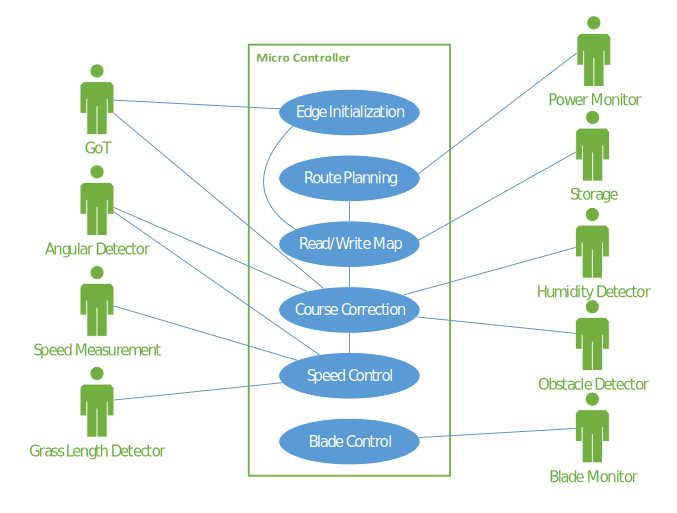
\includegraphics[scale=0.8]{figures/P5UseCase.pdf}
	\caption{Use-Case Diagram}
	\label{fig:usecase}
\end{figure}

\noindent
\newpage

The system, inside the controller, have 6 main functionalities and is affected by 9 different actors.

\subsection{Main Functionalities}

Functionalities are the functions that the system can do. Each Functionality can have more than one function in the system. The functionalities get input from actors and can be in association with other functionalities. 

\textbf{Edge Initialization}:
The \textit{Edge Initialization} gets input from the \textit{GoT} system and is associated with the \textit{Read/Write Map} functionality. The purpose of this function, is to calibrate the system to a new lawn. The function is making a edge map of the lawn. It used it to locate all the areas, where the lawn shall be mowed and where the lawn mower shall not drive. This is done, by manually moving the \textit{GoT} system's transmitter  along the edges of these areas. From the information about all the edges, the edge map is created and saved through the \textit{Read/Write Map} function.

\textbf{Route Planning}:
The \textit{Route Planning} gets input from the \textit{Power Monitor} and is associated with the \textit{Read/Write Map} functionality. The purpose of this function, is to plan the route for the lawn mower. The route is made from the information about where the lawn mower starts, the map of the lawn, which is made in the \textit{Edge Initialization} function. The map is loaded from the \textit{Storage} with the \textit{Read/Write Map} function. It also needs the battery level from the \textit{Power Monitor}. The route has to cover the whole lawn.

\textbf{Read/Write Map}:
The \textit{Read/Write Map} gets input from the \textit{Storage} and is associated with the \textit{Route Planning}, \textit{Course Correction} and the \textit{Edge Initialization} functionalities. This functionality communicates with the storage. In the \textit{Storage} the edge map from the \textit{Edge Initialization} function is saved and loaded from. The route from the \textit{Route Planning} is saved there to. The route is loaded and send to the \textit{Course Correction} functionality, when the system is driving.

\textbf{Course Correction}:
The \textit{Course Correction} gets input from the \textit{GoT} system, the \textit{Humidity Detector}, the \textit{Obstacle Detector} and the \textit{Angular Detector} and is associated with the \textit{Read/Write Map} and the \textit{Speed Control} functionalities. This function measures the surroundings of the lawn mower and makes corrections, in case of disturbances which might otherwise throw it off its route. The function makes the lawn mower stay on the route, which it get from the \textit{Read/Write Map} function, when the route can be followed. The \textit{Course Correction} is the main function behind the regulation of the movement of the lawn mower and sends these regulations to the \textit{Speed Control} function.

\textbf{Speed Control}:
The \textit{Speed Control} gets input from the \textit{Angular Detector}, the \textit{Grass Length Detector} and the \textit{Speed Measurement} and is associated with the \textit{Course Correction} functionality. The function's purpose, is to make sure that the lawn mower smoothly adapts the speed depending on the grass length, to get a more evenly cutting, and the curves of the route. This function controls the drive motor's speed, depending on route and regulation of the current speed.

\textbf{Blade Control}:
The \textit{Blade Control} gets input from the \textit{Blade Monitor}. The function's purpose, is keeping the blade rotational speed the same, to make an evenly cut. With the input from the \textit{Blade Monitor}, the \textit{Blade Control} regulate the speed to be constant.

\subsection{Actors}

A actor is a external system or component, that influence the system with inputs to the functionalities and/or gets output from them.

\textbf{Humidity Detector}:
The \textit{Humidity Detector} is connected to the functionality \textit{Course Correction}. This is a sensor that measures the humidity in the air. The system uses the information about the ambiant humidity level to see, whether it is too high to mow the lawn in or not, since wet grass can not be cut evenly and the cut of grass could damage the equipment. 

\textbf{GoT}:
The \textit{GoT} system is connected to the \textit{Course Correction} and \textit{Edge Initialization} functionalities. This system is used to get the lawn mower's position on the lawn. This position is sent to the controller, which uses the information to guide the lawn mower along its route.

\textbf{Storage}:
The \textit{Storage} is connected to the \textit{Read/Write Map} functionality. It uses a static storage to store the information about the edge map and route, which is made in the \textit{Edge Initialization} and \textit{Route Planning} functionalities. The \textit{Storage} will have the data saved, even if the system is turned off.

\textbf{Obstacle Detector}:
The \textit{Obstacle Detector} is connected to the \textit{Course Correction} functionality. This sensor detects, if there are any objects, which blocks the lawn mower's route. This sensor makes sure, that the lawn mower keeps a distance to any object, like a human or a dog that could interfere with its route.

\textbf{Angular Detector}:
The \textit{Angular Detector} is connected to the \textit{Course Correction} and \textit{Speed Control} functionalities. This sensor measures the angular position and movement of the lawn mower, whether it is intentional movement or if the lawn mower slips. This sensor is used as a feedback, to keep the lawn mower on the route.

\textbf{Grass Length Detector}:
The \textit{Grass Length Detector} is connected to the \textit{Speed Control} functionality. This sensor measure the  grass length, which affects the speed, at which the lawn mower should drive. If the grass is long and that it cuts, the lawn mower has to drive slower, to make sure that it doesn't get stuck in the grass and cut the grass evenly. 

\textbf{Power Monitor}:
The \textit{Power Monitor} is connected to the \textit{Route Planning} functionality. This sensor measures how much power  is left in the battery. This is needed, so that the lawn mower can drive back to its charging station, before the battery is empty.

\textbf{Blade Monitor}:
The \textit{Blade Monitor} is connected to the \textit{Blade Control} functionality. This sensor measures the rotational speed of the blade and send the information back to the \textit{Blade Control}, making a feedback loop.

\textbf{Speed Measurement}:
The \textit{Speed Measurement} is connected to the \textit{Speed Control} functionality. The sensor measure the speed, in which the lawn mower drive with. This information is send to the \textit{Speed Control} as feedback.
\section{Vehicle description}

\subsection{The vehicle in general}

The vehicle is composed of two tracks enveloping 4 wheels plus a gear wheel connected to the differential gear by a chain. The servo controls the steering of the vehicle by braking one track or another, so that the motor only control the absolut speed and not the turning. The differential gear is powered directly by the motor.\\
A Hall sensor is plugged on each gear wheel to control the speed of each belt.\\
A platform of the same size of the vehicle is mounted on the vehicle, to support the PCB, the battery, and the sensors used to control the path of the vehicle.\\

\todo{have to put the dimensions and weight of the vehicle}
\subsection{Drivetrain}
The drivetrain of a motored vehicle, is the components that transfer the rotational energy from the motor to the drive wheel of the vehicle. To understand the function of the different components, a picture of the vehicle can be seen on \figref{FullVehicle}. 

\begin{figure}[H]
	\centering
	\includegraphics[scale=.09]{figures/FullVehicle.png}
	\caption{Picure presenting all the elements used on the vehicle.}
	\label{FullVehicle}
\end{figure}
%\noindent 1) Motor\\2)Motor Gear\\3)Differential Gears\\4) Brakes\\5) Drive Wheel\\6) Belts\\7) Servo

To model this vehicle, a simplificated drawing of the vehicle is made. The drivetrain will contain the gear connected to the brushed DC motor, the differential gear box and the gears connected to the belts. The drivetrain is illustrated in \figref{vehicleDescriptionDriveTrain}.

\begin{figure}[H]
	\centering
	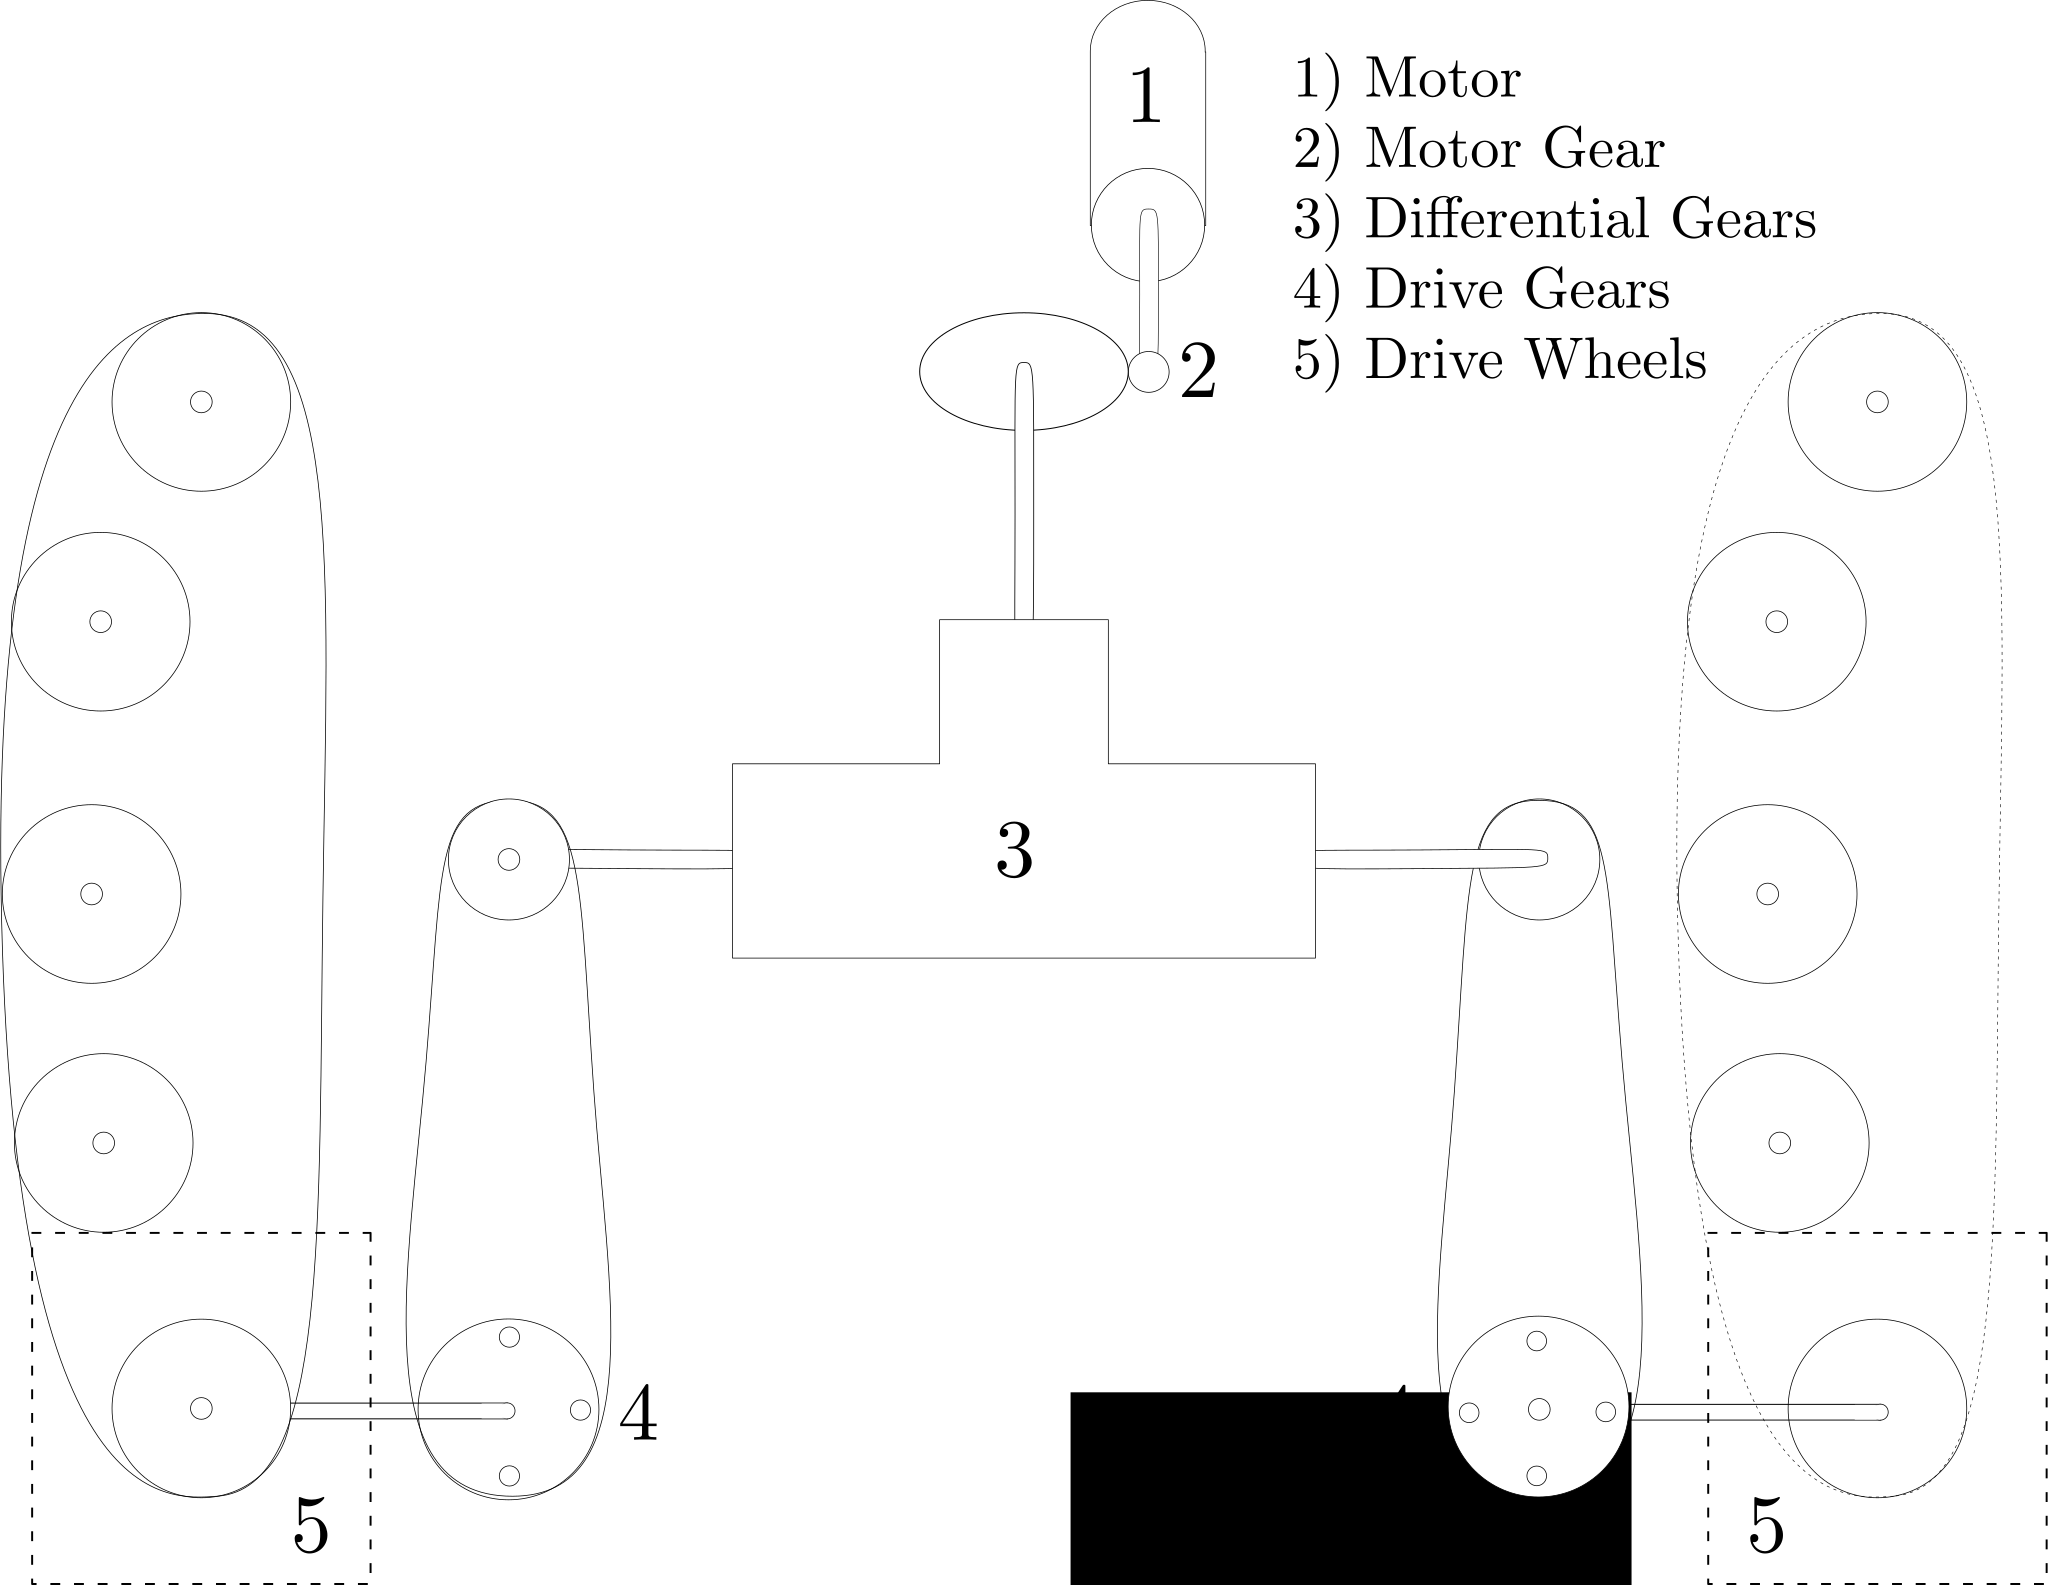
\includegraphics[scale=.25]{figures/vehicleDescriptionDriveTrain.pdf}
	\caption{Illustration of the drive train of the vehicle.}
	\label{vehicleDescriptionDriveTrain}
\end{figure}

In \figref{vehicleDescriptionDriveTrain} it can be seen that the motor delivers a force to the system through a the motor-shaft with a connecting gear. This gear is connected to the start of the drivetrain(1). From there the differential gear box is connected(2). From the differential gears two shafts are connected to a gear which transfers the velocity to the drive wheels(3).
From there the rotational velocity makes the drive-wheel turn, thus rotating the belts which are supported by four free wheels on each side(4). 

In the following segment, the differential gear box's function, seen in \figref{vehicleDescriptionDriveTrain}, is explained.            %----Drivetrain
\subsection{Differential gears} \label{sec:Differentialgears}

The differential gear box is located as the first component in the drivetrain, after the connection to the motor (Part 2 on \figref{vehicleDescriptionDriveTrain} in \secref{sec:Vehicledescription}).
When the servo is braking on one of the sides of the drivetrain, the differential gears transfer the rotational energy from this side to the other side. This minimize the lose of energy when braking. The extra speed, sent to the other belt that is not braking, will make the vehicle turn faster compared to a simple brake.

A differential gear system can be seen on \figref{diffGearLight}.

\begin{figure}[H]
	\centering
	\includegraphics[scale=0.7]{figures/diffGearLight}
	\caption{Illustration of a differential gear system. On the left, the resistance on each side is equal, so the spider gear does not rotates. On the right, the resistance on the left side is bigger than the one on the right side, so the spider gear rotates and transfer more rotational energy to the right side. \cite{MechanicalEngineering}}
	\label{diffGearLight}
\end{figure}

The differential gear system contains a ring gear (blue), a spider gear (green), two side gears connected to the rest of the system (red and yellow) and a pinion gear (not shown on picture) connected to the ring gear, that transfer the power from the motor to the system.\\

When the motor is running, the pinion gear transfer a rotational energy to the ring gear. The spider gear, fixed on to the ring gear, begins to rotate around the side gear. If the resistance on both side gears is the same, the same power is needed to rotate the gears. Therefore the spider gear will not rotate around its own axis and apply the same rotational energy to each side gear.\\

When the resistance on both sides is not the same, i.g. if one of the side is being brake on, the spider gear will rotate around is own axis. There is a bigger resistance on one side than on the other, so the side not braking will be easier to rotate. The ring gear and the spider gear are rotating at the same speed around the two side gears, but the spider gear will apply less rotational energy on the braking side than on the other side, because of it own rotation. In the case that the resistance on one side is infinite, as the spider gear is rotating at the same speed that the ring gear, the side gear on the none braking side will therefore rotate twice as fast, with the assumption that there is no loss in the system.\\

For the differential gear system on the vehicle, there is a more complete setup, shown on \figref{diffGearFull}
	%\caption{Illustration of the differential gear system on the vehicle \cite{MechanicalEngineering}}

\begin{minipage}{\linewidth}
      \centering
      \begin{minipage}{0.65\linewidth}
          \begin{figure}[H]
              \includegraphics[width=0.95\textwidth]{figures/diffGearFull}
              \caption{Illustration of the differential gear system on the vehicle \cite{MechanicalEngineering}}
              \label{diffGearFull}
          \end{figure}
      \end{minipage}
      \hspace{0.05\linewidth}
      \begin{minipage}{0.25\linewidth}
      		\begin{enumerate}
      			\item Pinion gear
      			\item Ring gear
      			\item Spider gears
      			\item Side gears
      		\end{enumerate}
      \end{minipage}
  \end{minipage}




%\begin{table} [H]
%\begin{tabular}{p{3cm} p{3cm}}

%\begin{figure}
%	\includegraphics[scale=0.7]{figures/diffGearFull}
%	\label{diffGearFull}
%\end{figure}

%&

%\begin{enumerate}
 % \item Hallo
%\end{enumerate}

%\end{tabular}
%\end{table}




%\begin{figure} [h]
%	\centering
%	\includegraphics[scale=0.7]{figures/diffGearFull}
%	\caption{Illustration of the differential gear system on the vehicle \cite{MechanicalEngineering}}
%	\label{diffGearFull}
%\end{figure}

Instead of only having one spider gear (the green gear on \figref{diffGearLight}) there is two for more reliability and solidity, shown in red on \figref{diffGearFull}. The system works in the same way as with one spider gear, with the pinion gear (1) transfering the power to the ring gear (2). The spider gears (3) fixed on the ring gear rotates the side gears (4) compared to their own resistance.

Now that the vehicle has been presented and its limits analysed, the prototype contraints can be considered to aim the functionnalities needed in this project.

\subsection{Things that maybe should be placed in this section}

When a permanent magnet DC motor is used, the inductor and resistor in the motor causes a time constant, that the PWM time period should be less than:

\begin{flalign}
T &< 2 \cdot \frac{L_a}{R_a} \cdot ln(1-\frac{P}{100})\unit{s}
\end{flalign}

Where P is the duty cycle in percent, and La is the inductance in the motor, and Ra is the resistance in the motor.

\subsection{Brakes}

 \begin{figure}[H]
	\centering
	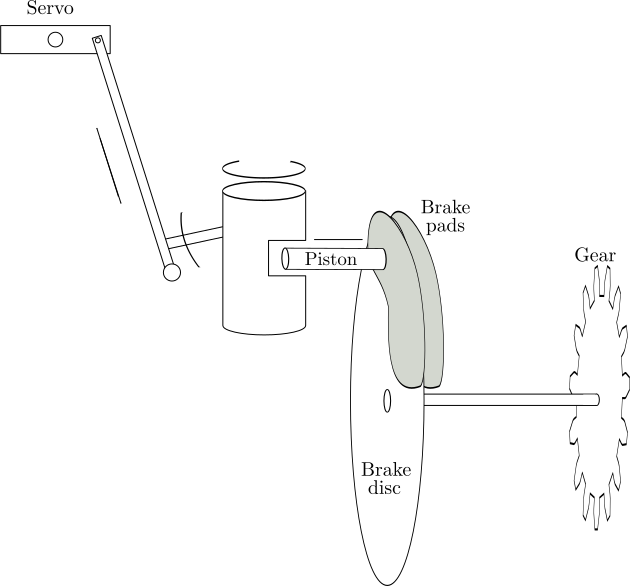
\includegraphics[scale=0.6]{figures/brakeDescription.pdf}
	\caption{Illustration of the brakes}
	\label{Brakes}
\end{figure}                %---- Steering
\subsection{Servo}
On the vehicle there is a servo, which is a S3003 by Futaba. \todo{Insert ref to the datasheet}
The servo is used for the steering of the vehicle. The servo controls the steering through breaking one of the belts, in part 3 on \figref{} in \secref{}, and transfer that power over to the other belt, thanks to the differential gear box.

The Servo is controlled by a PWM signal from the arduino card. The received PWM signal is converted into an angle by the servo to control the steering of the belts, as seen on \figref{timeVSangle}.

A mechanical arm is mounted on the servo and connected to the brakes of the tracks. When the servo rotates one way, it triggers the brakes more on one side and stop breaking at the other side, according to the value of the angle sent, through the PWM signal. This way, one of the belt will drive slower and the other belt drive faster, by the help of the differential gear system, which will make the vehicle turn, without decreasing the output power of the system.

\begin{figure}[H]
	\centering
	\includegraphics[scale=0.6]{figures/TimeVSangle.pdf}
	\caption{Convertion from time to angle by the servo}
	\label{timeVSangle}
\end{figure}

The servo reacts linearly to the PWM signal and the cycle of the signal is 30 milliseconds. To get the servo to be in neutral position at 90°, the servo needs a PWM signal of 4.83 \% (a period of 1450 microseconds). For 180°, it is 8.33 \% (a period of 2500 microseconds) and 1.67 \% (a period of 500 microseconds) for 0°. \\\todo{Insert ref to the datasheet}

When the servo brakes on one of the belt, the force, that should be lost in the breaking, is transfer to the other belt, by the differential gear system.
\subsection{Hall Sensor}

There are two hall sensors implemented on the vehicle, one on each belt. A hall sensor is a sensor that is activated when exposed to a magnetic field. The sensors are placed beside the front wheels, on which there are four magnets, placed so that there is a quarter of a turn between them. The hall sensor is illustrated on \figref{HallSensor}.

 \begin{figure}[H]
	\centering
	\includegraphics[scale=0.5]{figures/HallSensorSide_Forward_view.pdf}
	\caption{Illustration of the hall sensor.}
	\label{HallSensor}
\end{figure}

The Hall sensor will give a voltage output each time one of the magnets is in front of the hall sensor. This will give a signal each quarter of a turn of the wheel. As the distance between each magnets is not the same, the calculations will be taken for each magnets independently.
Knowing the time a turn of the wheel will take by measuring the time between four outputs, and the distance that the vehicle travels on that time, the speed of the vehicle can be calculated.

When the vehicle is starting to move, the first turn of the wheel can not be used because the calculations are made independently for each magnets. Therefore the speed can only be calculated by the first output of the second turn.\\\\


The two hall sensors are independent for being able to measure each belt when the vehicle turns through braking one track thanks to the servo.            %---- Hall Sensor
\section{Prototype Constraints}
Before the prototype can be established, some considerations have to be made in respect to the time limitations and the main scope of this semester. The aim of the project is to create a functional automated proof of concept lawn mower. The following section includes a brief description of the technology on which the prototype is constructed, along with argumentation for eliminated functionalities.

\subsection{Technology Base}
The technology which has been provided for the prototype is a tracked vehicle, seen on \figref{TrackedVehicle}. The vehicle comes with a brushed DC motor which provides power for rotation of the wheels connected to the belts. Furthermore a servo motor is used to control the ratio of the differential steering, by utilize breaks connected to the wheels. The tracked vehicle includes two hall sensors, one by each belt, which keeps track of the speed, of the belts, by measuring pulses from magnets mounted on the front wheels. The testing will take place in Aalborg University Vicon Room, where the GoT system is installed and calibrated with the appurtenant transmitter, which is mounted on the tracked vehicle during test.

\begin{figure}[H]
	\centering
	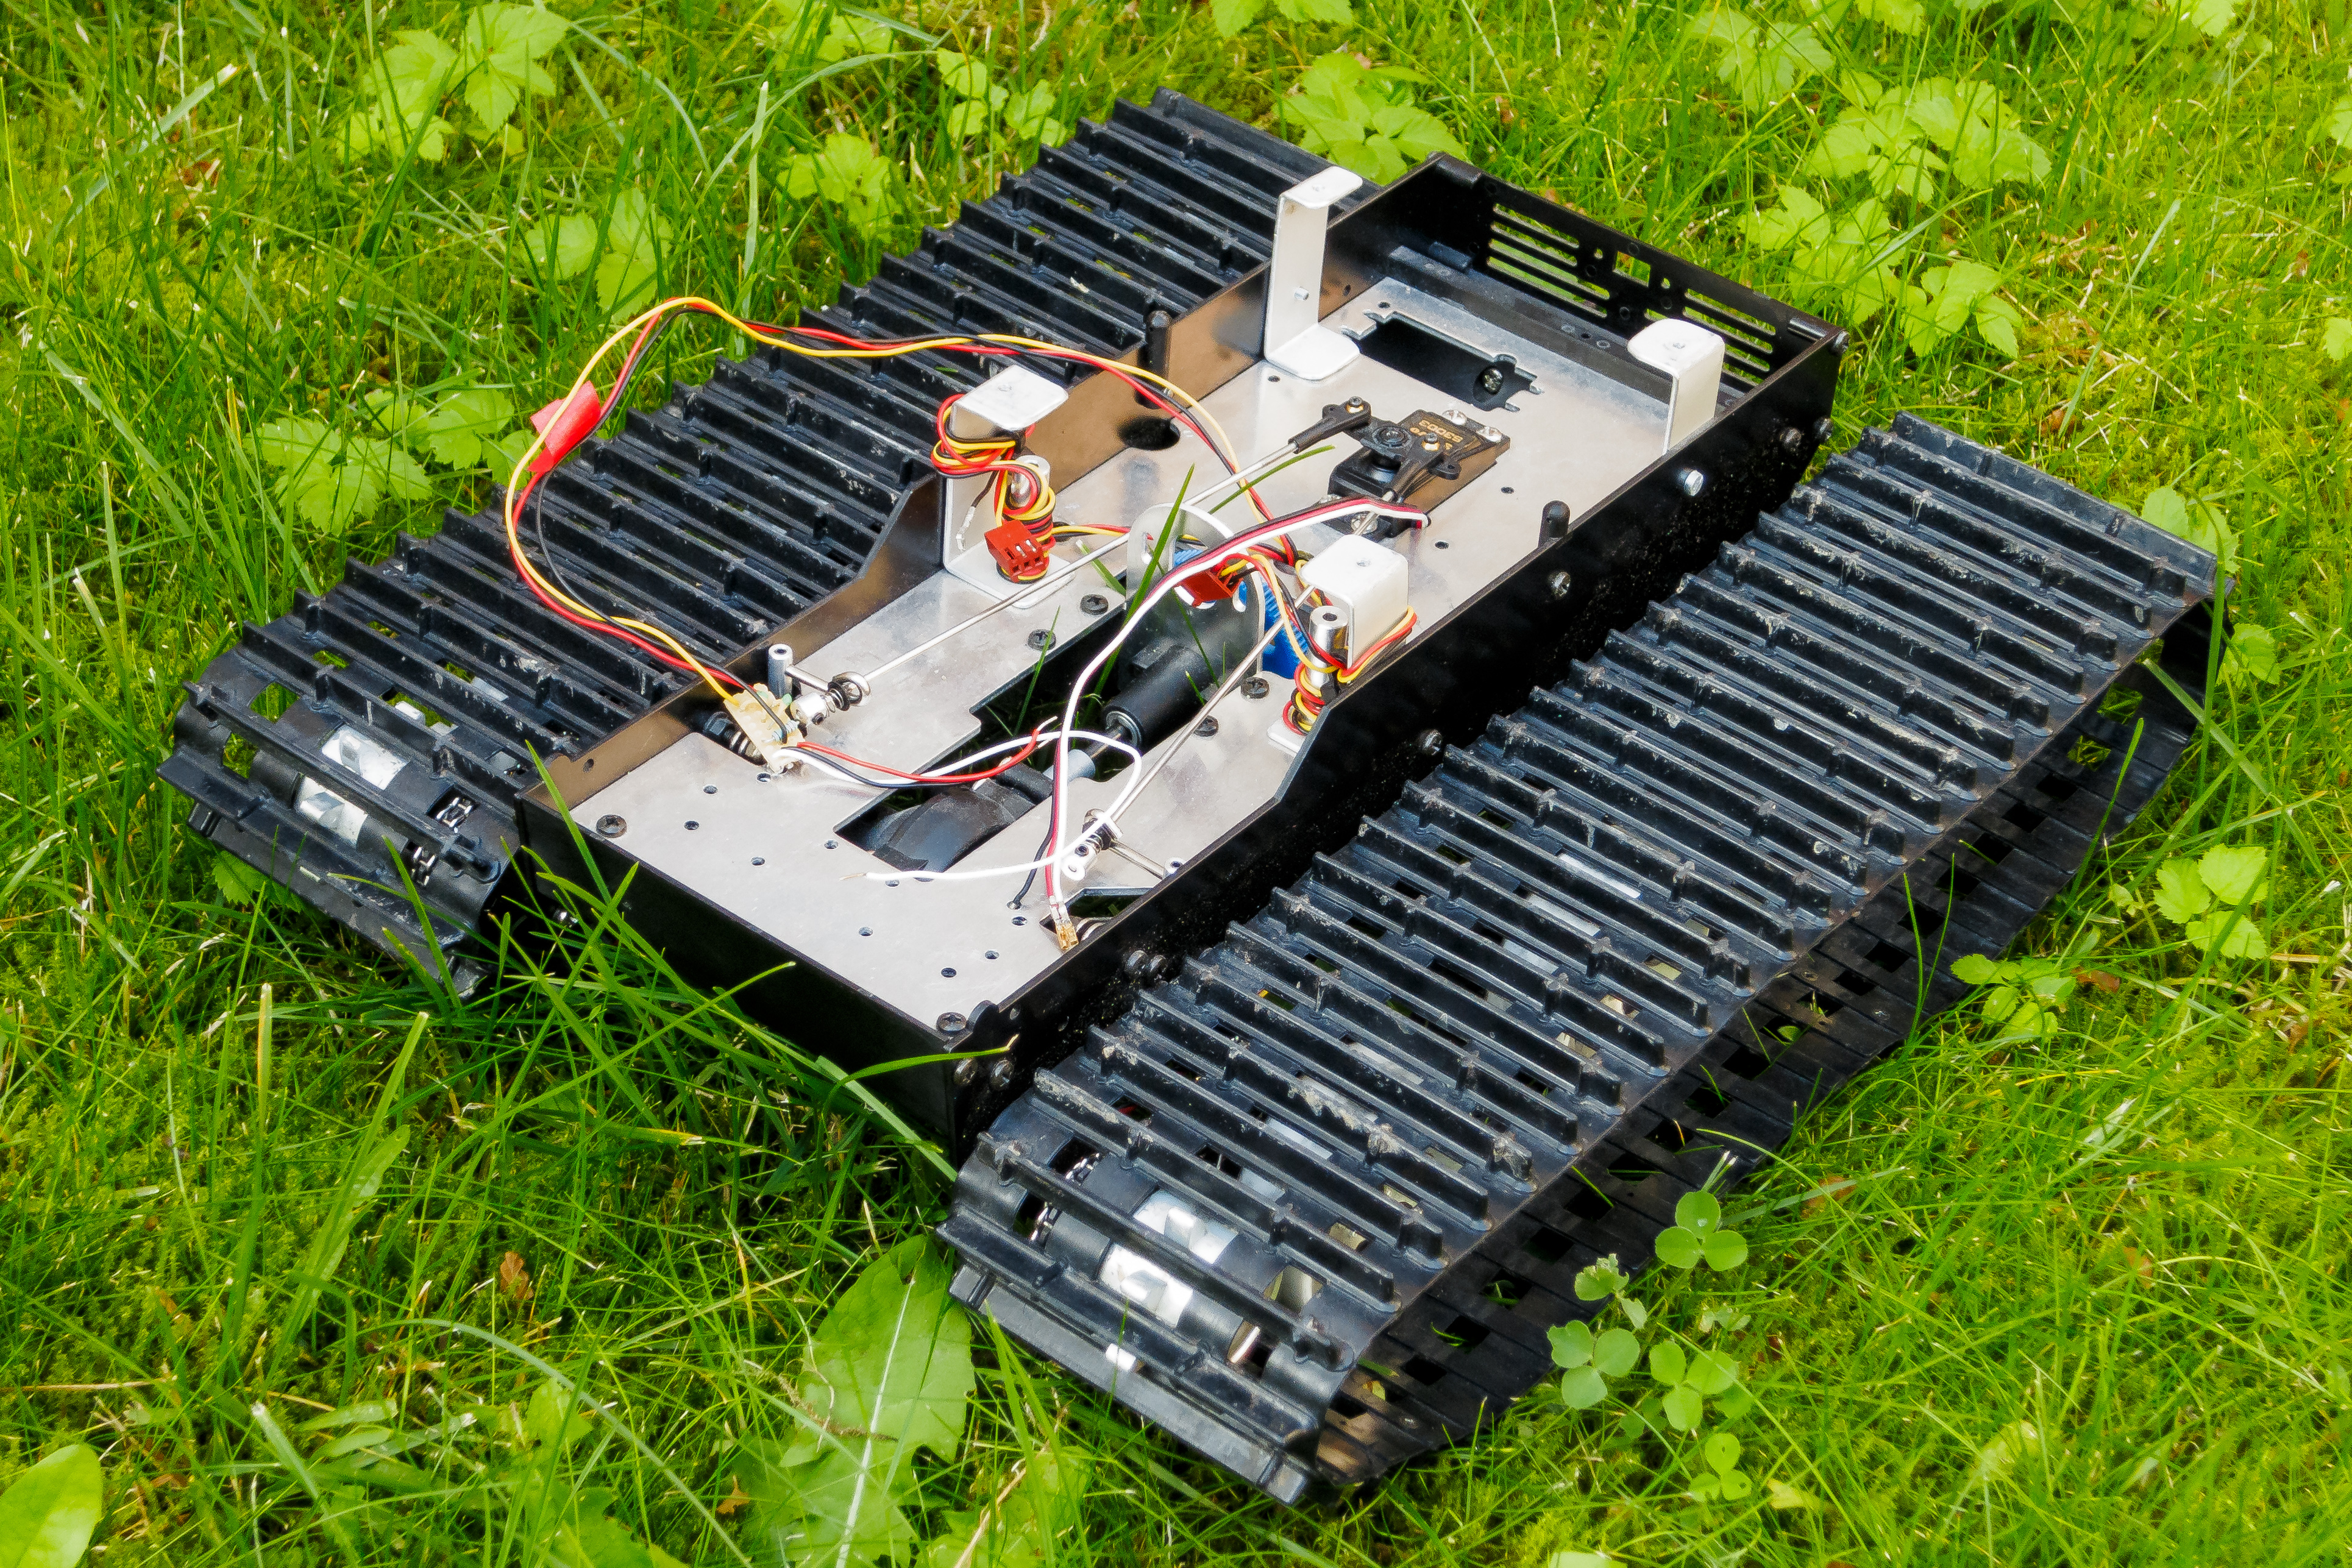
\includegraphics[scale=0.8]{figures/BeltVehicle.jpg}
	\caption{The provided track vehicle}
	\label{TrackedVehicle}
\end{figure}

\todo{datasheet of the vehicle}

\subsection{Grass Length Detection}
Detection of the grass length to control the speed of the lawn mower thus ensuring an evenly cut lawn, is a submodule which can be added at any time. Since it is not fatal for a working system and might even be unnecessary depending on time between each mowing of the lawn, it is decided to exclude this functionality from the initial design.

\subsection{Humidity Sensor}
As the lawn mower is supposed to work outside, it is important to consider that the grass could be humid. Since it is difficult to cut humid grass, a humidity sensor could be used to warn the system of the humidity. Thus the system could go back to the charging station. However, the prototype will only be tested indoor, so this type of sensor will not be necessary in a prototype design.

\subsection{Obstacle Avoidance}
The lawn movers path might not always be clear, e.g. garden tools, tables or moving objects could be in the way. The vehicle should be aware of what is in front of it at any time, to correct its path and get around the obstacle if necessary. To avoid this the sensor could be a pushing button to detect a solid object or an ultrasound detector if the object is fragile.
As the aim of the project is to control the path of the vehicle by using angular positioning sensors, a proximity sensor will not be included. Static objects could be registered on the map to avoid these issues.\\\\
Furthermore the edge mapping functionality will not be included in the project which instead will focus on a quadratic map predefined in the test room.

\subsection{Power Monitoring}
Power monitoring could be implemented by measuring the voltage across the batteries, to ensure that the lawn mower is not running out of power, and to ensure the vehicles calculated route passes the charging station before the power runs too low.
This and the charging station will not be in the prototype, since it is beyond the scope of the project this semester and is not crucial for a working prototype.
 %---- Prototype Constraints
\section{Prototype, Interfaces and Submodules} \label{Finalprototype}
%The overall functionalities for the project have been limited, due to time limitations and to focus on the scope of the project. In this project a prototype will therefore be made to show the main functionalities necessary to make an automated vehicle containing principles for lawn mowing.
%In short, the final prototype includes a regulator, which will make it possible to follow a path from A to B. It is able to continue if the wireless connection is lost between the prototype and the GoT system for some duration. Furthermore it is able to plan a route within a given area and store these calculated data points locally, on the vehicle. The rough outline of the design is shown in \figref{fig:systemOverview1} to give an idea of the final prototype setup.

%\begin{figure}[H]
%	\centering
%	\includegraphics[scale=.9]{figures/systemOverview1}
%	\caption{Overview of the system prototype}
%	\label{fig:systemOverview1}
%\end{figure}

%The GoT system provides the vehicle with coordinates, which is utilized in course correction in combination with the map supplied from storage, to follow the route. In course correction lies also control between coordinates given by the GoT system and the storage, this is regulated through use of angular position and movement supplied by the angular sensors. The speed control gets an input from the course correction, the speed given is then held through regulation again using input from angular sensors, in this case specifically acceleration.


%Previously the rough prototype design is presented. To provide a more broad overview of the system, an exploded view of functionalities, their submodules and interfaces is presented in \figref{fig:systemOverview2}.

The overall functionalities for the project have been constrained from the Use-Case \secref{sec:UseCase}, due to time limitations and to focus on the main scope of the semester. A prototype is therefore made to illustrate the main functionalities necessary to make an automated vehicle, containing principles for lawn mowing.

The final prototype includes a regulator, which will make it possible to follow a path from A to B. It is able to continue if the wireless connection is lost between the prototype and the GoT system for some duration. The outline of the design is shown in \figref{fig:systemOverview2} to give an idea of the final prototype setup. In this section, the different functional blocks are put forth along with the interfaces describing the interaction between them.

\begin{figure}[H]
	\centering
	\includegraphics[scale=.9]{figures/systemOverview2}
	\caption{Overview of the software and electronic parts of the system prototype, where the gray modules are hardware and the white are software. The dotted lines are wireless signals while the others are wire signals}
	\label{fig:systemOverview2}
\end{figure}

\subsection{Modules}
In the following all the modules from the system prototype which needs further explanation are described to obtain a basic understanding of the prototype.

%\subsubsection{GoT System}
%%The GoT satellites is placed in the area in which the vehicle needs to operate. These satellites receives information from the vehicle. The time which the vehicles transmitter sends out bursts is received by the GoT master. Furthermore the time which the satellites receives the information send from the vehicles transmitter is transmitted to the GoT master. The GoT master then relays the information received from the vehicle directly to the 
%
%The \textit{GoT Transmitter} placed on the vehicle transmits a signal containing the time at which it send the ultra sound signal to the \textit{GoT Satellites} to the \textit{GoT Master}. The satellites transmit the signal recieved to the master as soon as they recieve it. The master then relays those informations to the \textit{GoT on Computer} that will calculate the position of the car.

\textbf{Computer and Position Decoder:}
The computer handles the calculation of the current position of the vehicle \appref{GoTDescription}. If a packet is disturbed or sent incorrectly it should be possible to detect it, so invalid data is not used by the prototype. It may occur that the coordinates which are sent from the GoT system is out of sensible range, e.g the coordinate transmitted jumps from one location to a location which is unrealistic, for the vehicle to reach in the amount of time between received coordinates. In this event the out of range coordinate should also be disregarded. The computer must compile a package containg the coordinates. The position decoder must be able to decode the send package.

\textbf{Course Correction:}
This module receives the vehicles position from the GoT and the next destination on the path, which is located in the storage. These informations constitutes a path segment on which it is the course correction's task to stay. To accomplish this it receives the angle and the speed of the vehicle, and uses this information to correct its course along the current path segment.

\textbf{Read/Write Map:}
This module handles the writing of coordinates to the nonvolatile storage device, as well as the reading of next desired destination from the stored map.

\textbf{Speed Control:}
This module retrieves the speed of the vehicle from the Get Speed module. This is used, through control, to obtain a steady speed. Furthermore it handles any request of change in speed delivered by the course correction.

%\subsubsection{Edge Map}
%The first time the user will initialise the lawn mower, an \textit{Edge Map} will be created thanks to the GoT system. This edge map will determine the areas that the car is allowed to go or not, in regards of specifications or objects on the lawn.  

%\subsubsection{Route Planning}
%The Route Planning module calculates a route from the points gathered from the Edge Map. The route will be in straight lanes, as in the Bosch Logicut system \secref{roboMowers}, to guarantee that the whole lawn is cut.

%\subsubsection{Angular Sensors}
%The angular position is measured thanks to the \textit{Angular Sensors}, that will send data to the submodule \textit{Get Angle}, in charge to send the angle to the Speed Control and to the Course Correction submodule.

\subsection{Interfaces}
%- To Tom and Rasmus \newline
%In the subsection an explanation of the different interfaces between the modules is made. We have thought about making it like a high layer interface, where we only explain what we need the different modules to give each other. Like one module needs to get the map edge, i.e. coordinates, but since it is this early in the report and it would be more overview by writing map edge rather than coordinates. But as you can see in \figref{fig:systemOverview2} the layers of information are different, one is raw angle data and another time send. Is this okay or should we change something else?
%\indent
%The interfaces of the system is very important when designing each of the adjacent submodules. The existing interfaces as well as the ones presumed are also important in the process of analyzing the system capabilities width focus on requirements of the prototype. Width that in mind follows a brief review of the interfaces between each submodule.
In this section a high layer interface between the modules will be presented. This provides information for designing each of the adjacent submodules individually.

\textbf{8 - Package Containing Position:}
The data communicated from the GoT system to the vehicle contains the last recorded position of the vehicle. This position is presented in the form of an x- and a y-coordinate, which must be included in the data package. Additionally each package must contain decode information for the receiver, including how to separate each package along with error handling.

\textbf{7 \& 4 - Angle/Servo Control Signal \& PWM Signal:}
Course correction will ask the vehicle to turn or make small adjustments of the angle. This angle is realized through the servo motor which breaks on either belt aproprite to the required angle. For the servo to understand the angle the servo driver must translate it into a PWM signal, which makes the servo turn to a specific position for each pulse width.

\textbf{2 \& 1 - Angle \& Raw Angle Data:}

\textbf{6, 5 \& 4 - Desired Speed, Motor Control Signal \& PWM Signal:}

\textbf{11 \& 3 - Hall Sensor Pulses \& Belt Speed:}

\textbf{13 - Route Coordinates:}






%Route Planning, Storage and Read/Write Map Interfaces:
%The Edge Map submodule sends the Map edge to Route Planning, that will send a Route to Read/Write Map. The Route to follow will then be transmited to the Course Correction submodule for a path correction, and to the Storage for saving.

%\textbf{Speed Control Interfaces:}
%The Hall Sensors send Hall sensor pulses to the submodule Get Speed, that will process it to transmit the Belt speed to the Speed Control. A PWM signal containing the new wanted speed will then be sent to the Motor Driver, wich will convert it to the final Motor control signal and sent it to the Drive Motor.
%
%\textbf{Angular Sensors Interfaces:}
%The Angular Sensors will send a Raw angle data to the submodule  Get Angles, that will process it and send the Processed angle data to Course Correction.
%
%\textbf{Course Correction Interfaces:}
%The Course Correction submodule receives the Position and Time from the Wireless Module, the Route to follow from Read/Write Map, and the Processed angle data from Get Angles. With all those information, a decision will be sent to the Speed Control through the Desired speed, and to the Servo Motor with an Angle/servo control signal.

Now that the vehicle had been described and the prototype defined, the modeling of the vehicle can be made.


%---------------------------------------------------------------------------------------------------------------------------\\
%REWRITE THIS SCRAMBLED VERSION OF THE ABOVE TWO SUBSECTIONS \todo{rewrite in the above section and delete these subsections}\\
%---------------------------------------------------------------------------------------------------------------------------
%
%\subsubsection{GoT Satellites, Master and GoT Ultra Sound \& Radio Link}
%\indent
%A number of GoT Satellites are placed in the corners of the area in which the vehicle is to operate. These Satellites receive ultra sound signal from the GoT device placed on the vehicle. The time in which each ultrasound signal is received is passed through a wireless connection from the satellites to the GoT master. The GoT master then pairs this information with the time the ultra sound signal was send from the vehicle which it receives via radio link from the GoT device on the vehicle. After collecting the information, the GoT master sends a calculated position and along with a time stamp to the computer handling GoT.
%
%\subsubsection{Wireless Modules}
%\indent
%%The wireless modules serves the purpose of transmitting the calculated coordinates from the GoT system to the vehicle.
%
%\subsubsection{Edge Map, Route Planning, Read/Write Map and Storage}
%\indent
%%The route planning functionality receives the hard coded edge positions from edge map. Using this information the route is then planned and saved in the storage through the read/write map functionality.
%
%\subsubsection{Gyro, Accelerometer, Magnetometer, Speed Control and Course Correction}
%\indent
%%Gyro along with magnetometer is used for angular position of the vehicle. This is passed to the course correction through the get angle functionality. Here it is used as to correct the orientation of the vehicle on its path. The accelerometer also channels through the get angle functionality. The angular acceleration is then used for correction of the speed.
%
%\subsubsection{Hall Sensor}
%\indent
%%The speed control also receives input from the hall sensors through the get speed functionality, where the inputs from the hall sensors are translated to speed of the vehicle's belts. This information is then used in speed control to regulate the speed.
%
%\subsubsection{Servo Motor}
%\indent
%%The servo motor receives an angle/servo control signal from course correction. This angle equals a given amount of breaking on either of the two belts, which then through the differential gearing translate into steering and thus correction of the course of the vehicle.
%
%\subsubsection{Motor Driver and Drive Motor}
%\indent
%%The drive motor takes a motor control signal from the motor driver provided by the speed control. The control signal from speed control is a PWM signal.            %---- Prototype

%---------- Chapter 3 ---------------------------------------- Requirements
\chapter{Prototype Requirements} \label{Requirements}
Based on the preanalysis, the use case, system description and prototype, it is possible to establish requirements for the prototype.

\begin{enumerate}
%\item \textbf{It shall be possible to track the vehicle's position}
%	\begin{itemize}
%	\item[] why and from where?
%	\end{itemize}
\item \textbf{It shall be possible for the vehicle to receive its own location wirelessly from the GoT system, through a computer.}
	\begin{itemize}
	\item[] The vehicle needs to be able to receive its own location, additionally, it should be wireless so the vehicle can drive without cables attached, and thereby be able to move freely, \secref{Finalprototype}
	\end{itemize}
\item \textbf{It shall be possible for the prototype to disregard incorrect packets transmitted from the computer}
	\begin{itemize}
	\item[] To ensure that invalid data is not utilized, \secref{Finalprototype}
	\end{itemize}
	\item \textbf{The prototype must be able to disregard erroneous coordinates sent from the GoT system}
	\begin{itemize}
	\item[] If the GoT system delivers an unrealistic coordinate, e.g. created by noise, to the vehicle, \secref{Finalprototype}.
	\end{itemize}
\item \textbf{The prototype must be able to access the route, which it has to follow, from a storage space located on the vehicle}
	\begin{itemize}
	\item[] To simulate the use-case, see \secref{sec:UseCase}, the route needs to be stored on the vehicle, and thereby making it accessible for the functionality course correction, \secref{Finalprototype}.
	\end{itemize}
\item \textbf{The prototype must be able to shut down, if the battery voltage is below its cut-off specification}
	\begin{itemize}
	\item[] To ensure the battery is not damaged, \secref{Finalprototype}.
	\end{itemize}
\item \textbf{It shall be possible for the prototype to follow a predetermined route}
	\begin{itemize}
	\item[] This is to simulate a lawn mower, which is able to cut grass by following a route, \secref{sec:PrototypeConstraints}
	\end{itemize}
\item \textbf{It shall be possible for the prototype to return to the predetermined route if disturbed}
	\begin{itemize}
	\item[] E.g. if the vehicle slips or is moved, \secref{sec:UseCase}
	\end{itemize}
\item \textbf{The prototype shall be able to keep a velocity on 1,4 $m \cdot s^{-1}$, when going up - or downhill and when turning}
	\begin{itemize}
	\item[] To ensure an evenly cut of the grass, \secref{sec:UseCase}
	\end{itemize}
\end{enumerate}

Based on the established requirements it is now possible to design a prototype of an autonomous vehicle.


%%% Part 2 %%%
\part{Design \& Implementation}
%---------- Chapter 4 ---------------------------------------- Hardware considerations
%% TODO : Move files in appropriate folders when nobody is working on it
\chapter{Hardware and Software\\ Considerations}

The description of the vehicle have been made, and the protoype of the system established. The requirements have been decided regarding the equipment given. To meet them, the hardware and software choice have to be considered. In this section, an explanation of the hardware choices will be made for the sensors, drivers, and others materials needed with their implementation. In another part and to be able to use those hardware parts, the software process will be described, along with the choice of the kernel used and the schedulling optimized.
\section{Hardware choice} \label{Hardwarechoice}
From the Requirements \todo{Ref to requirements}, the hardware components are chosen for the prototype. Beside the requirements for each components, there is considered the availability of the component and the implementation of the component in the system.

%%%%%%%%%%%%%%%%%%%%%%%%%%%%%%%%%%%%%%%%%%%%%%%%%%%%%

\subsection{Microcontroller}
The microcontroller is the brain of the system. The purpose of the controller is to connect all the other hardware component, contain the software script of the system and control the rest of the system, with help of signals, controlled by the script.

The requirements for the microcontroller are:
\begin{itemize}
\item Have a CPU, that have a frequency greater than XX. \todo{Number}
\item Having I/O connections, both digital and analogue.
\item Having 5 free timers, to control different part of the system parallel with each other.
\item Having output connections, that can transmit PWM signals.
\item Can be powered by an external power source.
\end{itemize} 

\subsubsection{Arduino Mega 2560}
Arduino microcontroller is 

%https://www.arduino.cc/en/Main/ArduinoBoardMega2560

%%%%%%%%%%%%%%%%%%%%%%%%%%%%%%%%%%%%%%%%%%%%%%%%%%%%%

\subsection{Storage}
The storage is used for saving the edge map and the route for the vehicle \todo{Ref to last place this is mention}. This data have to be saved from use to use of the vehicle. 

The requirements for the storage are:
\begin{itemize}
\item Have to be controlled by the microcontroller.
\item The data shall be retrievable, after a power cut to the storage. \todo{Re formulate}
\item Have a storage of XX bytes. \todo{Number}
\item The transfer speed is greater than XX bytes per second. \todo{Number}
\end{itemize}

\subsubsection{SD card} \label{SDcard}
Secure Data card (SD card) is a non-volatile memory card. This give it the feature that the data will not be lost at a power cut off. 

It comes in various storage sizes, from 1 GB to 2 TB, depending which type of SD card it is. There is 3 types of SD card, the standard capacity (SDSC), the high capacity (SDHC) and the extended capacity (SDXC). The  difference between the different type, is the file system use on the card and the capacity cap. With the requirement of a storage size on XX bytes, the SDSC big enough with a capacity cap on 2 GB. 

The transfer speed for a SDSC card is 2 MB/s the slowest a card can maximum go by. With the requirement of a transfer speed greater than, the SDSC card is fast enough. 

To use the SDSC card, it have to setup up with 7 connections to a controller, see \figref{SDcardpinout}. The setup of the SD card is different, depended on which mode that is used. 

\begin{minipage}{\linewidth}
      \centering
      \begin{minipage}{0.30\linewidth}
          \begin{figure}[H]
              \includegraphics[width=0.95\textwidth]{figures/sdcardpinout}
              \caption{Illustration of a micro size SD card.} % http://elasticsheep.com/2010/01/reading-an-sd-card-with-an-atmega168/
              \label{SDcardpinout}
          \end{figure}
      \end{minipage}
      \hspace{0.03\linewidth}
      \begin{minipage}{0.65\linewidth}
			\begin{table} [H]
				\begin{tabular}{|l|l|l|l|}
				
				
\hline
\textbf{Pin} & \textbf{SPI}  & \textbf{One bit} 	& 	\textbf{Four bit}  \\
\hline
1			 &	Unused		 &	Unused			    &	Data 2			   \\
\hline
2			 &	Card Select	 &	Card Detection		&	Data 3			   \\
\hline
3			 &	Data in		 &	\begin{tabular}{@{}c@{}} Command \&  \\Response \end{tabular}  &	\begin{tabular}{@{}c@{}} Command \&  \\Response \end{tabular} \\
\hline
4			 &	Power		 &	Power			    &	Power			   \\
\hline
5			 &	Serial clock &	Serial clock		&	Serial clock	   \\
\hline
6			 &	Ground		 &	Ground			    &	Ground			   \\
\hline
7			 &	Data out	 &	Data 0			    &	Data 0			   \\
\hline
8			 &	Unused		 &	Unused			    &	Data 1			   \\
\hline

					
					
				\end{tabular}							
			\end{table}			
      \end{minipage}
  \end{minipage}
  \todo{Talk with niels about table}



The power needed for a SD card is 3.3 volts\todo{Check up with thomas}. There is three setups for the SD card: SPI, one bit and four bit. With the SPI setup, the communication between the SD card and the micro controller is on two lines. The SPI mode is the most used one for embedded systems.
With the one bit setup, the commands between the SD card and micro controller is happening on line the data is send another line. With the four bit setup, there is connected three more data lines.

In the project, the SPI setup will be used, as it is the most used method and there is not needed the extra transfer speed from the four bit setup.


A SDSC card, with a SPI setup, will be use for the project, as it have a capacity and transfer speed that meets the requirements. The data will be saved, if the power is cut off. The last requirement, the connections to the microcontroller, is possible, because the Arduino Mega 2560 controller contains  digital I/O pins, that can be use for the SPI setup for the SD card.

%https://www.sdcard.org/developers/overview/capacity/index.html
%https://www.sdcard.org/developers/overview/speed_class/
%%%%%%%%%%%%%%%%%%%%%%%%%%%%%%%%%%%%%%%%%%%%%%%%%%%%%

\subsection{Motor Driver}
The motor driver is the connection between the microcontroller, the power supply and the motor. The component is used, to separate the low power components, i.e. the microcontroller, and the high power components, i.e. the motor.

The requirements for the motor driver are:
\begin{itemize}
\item Have to be controlled by the microcontroller.
\item Can be powered by an external power source.
\item Can handle up to 7.2 volts. \todo{Number}
\item Can power the motor in both direction.
\end{itemize}

\subsubsection{Pololu Dual VNH5019}

%%%%%%%%%%%%%%%%%%%%%%%%%%%%%%%%%%%%%%%%%%%%%%%%%%%%%

\subsection{Power Supply}
The external power supply have to both power the motor, which need a high voltage and high power and the other components, which needs low voltage and low power.

The requirements for the power supply are:
\begin{itemize}
\item Voltage output of 7.2 volts. \todo{Number}
\item Deliverer a stable power output.
\item Can run the motor at full speed for XX. \todo{Number}
\end{itemize}

\subsubsection{Battery pack}
For the project there will be used a rechargeable battery pack on 7.2 volts. As the prototype is not set to run a long time, less than XX, a normal battery pack used for XX \todo{Thomas again} can be used. The battery pack will deliverer a stable power output as long as the power level in the battery pack. In appendix XX \todo{Make test}, it can be seen, that the battery pack can deliverer a stable power output for XX minutes.

%%%%%%%%%%%%%%%%%%%%%%%%%%%%%%%%%%%%%%%%%%%%%%%%%%%%%

\subsection{Wireless communication}
The data from the GOT system is send to the microcontroller with this component. The transmitter will be located at the computer for the GOT system and the receiver on the vehicle.

The requirements for the wireless communication components are:
\begin{itemize}
\item Have to be controlled by the microcontroller.
\item Have a reach greater than XX. \todo{Number}
\item Powered by an external power supply.
\item The transfer speed is greater than XX bytes per second. \todo{Number}
\item Have a loss of bits smaller than XX. \todo{Is this needed and what number}
\item Can be implemented in the GOT code.
\end{itemize}

\subsubsection{Xbee}
Xbee are small radio moduls, that is easy to set up. To run the Xbee moduls, there is needed a power on 3.3 volts, a ground and a UART on 3.3 volts. It have a transfer speed up to 115.2 kilobits per second and have a reach up to 100 meters indoor and 300 meters outdoor. It transmit with 1 millivolt (0 dBm) and can receive downto -96 dBm. It transmit at a 2.4 GHz frequency \todo{Check with thomas}. The Xbee is al set from the start with the under level for transmission, so there is only needed a presentation layer for a protocol to work with the transmission.

%http://www.digi.com/products/xbee-rf-solutions/modules/xbee-digimesh-2-4#specifications

%%%%%%%%%%%%%%%%%%%%%%%%%%%%%%%%%%%%%%%%%%%%%%%%%%%%%

\subsection{Angular sensor}
The angular sensor is used in the feedback for the control system.

The requirements for the angular sensor are:
\begin{itemize}
\item Have to be controlled by the microcontroller.
\item Having a sampling frequency greater than XX. \todo{Number}
\item Having a latency smaller than XX. \todo{Number}
\item Powered by an external power supply.
\end{itemize}

\subsubsection{HMC5883L}

%%%%%%%%%%%%%%%%%%%%%%%%%%%%%%%%%%%%%%%%%%%%%%%%%%%%%

%1. Micro controller
%- Timers
%- In and out pins (Analogue or digital???)
%- Can be powered by external power source
%- Frequency on the CPU
%- Serial???
%
%2. SD card
%- Saved, even when the there is a power cut
%- Size
%- Speed of transfer
%
%3. Motor driver
%- External powers source
%- Can handle 7 volts (Motor req)
%- Can power the motor both ways
%
%4. Batteries
%- Deliver a stable power
%- 7 Volts
%- Drive time
%
%5. Xbee
%- Transfer speed
%- Communication with the micro controller
%- Distance of sending radius
%- Reliability
%- Powered by batteries or micro controller
%
%6. Hall sensor
%- Sampling frequency
%- Reliability
%- Latency
%
%7. Angular sensor
%- Sampling frequency
%- Reliability
%- Latency
%
%Note: Insert speed of sampling in the GOT

%Pins on the arduino
%SD card (4 I/O)
%Xbee (1 TX and 1 RX)
%Hall (2 I/O)
%Angular (1 SDL and 1 SDA)
%Servo (1 PWM)
%Motor (1 PWM)


% Something about philips stuff
\section{Hardware Implementation}
With the hardware components being chosen, it is necessary to assemble them, ensure that they are compatible for communication with the microcontroller, and that they receive the appropriate electrical power. Other implementation considerations also have to be considered. e.g , the voltage divider for the power monitor.
\subsection{Microcontroller peripherals}
Before choosing which pins on the Arduino Mega to connect the various hardware to, the peripherals\footnote{Hardware modules, such as timers, UARTs, etc.} in the microcontroller needs to be evaluated (each peripheral is only available on certain pins). First, the timers are considered. The microcontroller has 6 hardware timers, Timer 0 to Timer 5.

Timer 0 is reserved by the Arduino for it's internal time keeping functions, and not to be touched \cite{ArduinoPWM}. This leaves 5 timers, that can be used freely.

It would be advantageous to utilize the input capture\footnote{An input capture timer samples a free running counter, whenever triggered by  an external event} functionality of the timers to read the hall sensors, since it will provide a hardware generated timestamp, and be independent of software latency. After examining the Arduino Mega pinout, \appref{megaPinout}, it is seen that only Timer 4 and 5 have their input capture pins available on the board (ICP4 and ICP5). These are therefore chosen for the two hall sensors.
   
The real-time operating system needs a timer, for running its scheduler. Timer 1 is chosen for this, for no other reason than it being the default setting.

This leaves Timer 2 and 3. According to \cite{Atmega}, Timer 2 is an 8 bit timer, and Timer 3 is 16 bit. 

Timer 3 is chosen for the PWM signal sent to the servo. This, because the higher resolution makes it easier to generate the short duty cycles required by the servo (\si{500\ \mu s} to \si{2500\ \mu s} on-time, in a \si{30\ ms} period, see \subsecref{Servo})

The last timer is chosen for the PWM signal to the DC-motor.

As the timers have now been designated, the next step is to assign the various serial ports. This is done as shown on \figref{MegaSetup}. Considerations about the powering of the hardware modules is seen in \secref{sec:elecConsiderations}.	


\begin{figure}[H]
	\centering
	\includegraphics[scale=0.75]{figures/MegaSetup.pdf}
	\caption{Connections between the different hardware components and the Arduino.}
	\label{MegaSetup}
\end{figure}

The XBee module needs to connect to a serial port, and UART3 is chosen, as it makes it easier to route the PCB traces. UART3 is located at pins 0 and 1. 

The SD card needs an SPI connection, and must therefore be connected to the SPI pins 50, 51, 52 and 53. 

The "9 Degrees of Freedom" board needs an $\text{I}^2\text{C}$ connection, and has to be connected to the Arduino's $\text{I}^2\text{C}$ pins 20 and 21. 

The PWM signals sent to the motor and servo can be set to any of the PWM pins. For easier routing, pin 9 for the motor and pin 5 for the servo is selected.

The input from the hall sensors will be measured by the input capture pins (ICP4 and ICP5), to which Timer 4 and Timer 5 are connected. On the Arduino board, it corresponds to the pins 46 and 47.

Lastly, the voltage divider used for the power monitoring is connected to an analogue pin chosen to be pin A9.

As all hardware modules have now been assigned pins on the Arduino, the electrical requirements of each module will now be considered.

\subsection{Electrical considerations}\label{sec:elecConsiderations}

Before connecting hardware modules to the Arduino pins, signal voltage levels also need to be considered:

\begin{itemize}
\item The Arduino Mega 2560 itself uses 5V logic levels.\cite{MegaInfo}
\item The "9 Degrees of Freedom" board needs \SI{3,3}{V}-\SI{16}{V} supply and $\SI{3,3}{V}$ logic levels. \cite{9dog}
\item The servo needs $\SI{4,8}{V}$ to \si{6\ V} supply voltage and signal levels.\cite{futaba}
\item The SD card needs $\SI{3,3}{V}$ supply voltage and signal levels, see \subsecref{SDcard}.
\item The Hall sensors needs $\SI{3,5}{V}$ to \si{24\ V} supply, and a pull up resistor to define the logic level.
\cite{HallDS}
\item The XBee module needs $\SI{3,3}{V}$ supply voltage and signal levels.
\subsecref{Xbee}
\end{itemize} 

The Arduino has regulated 5V and $\SI{3,3}{V}$ supply rails available, which will be used to power the respectable hardware modules. As the servo can potentially draw a lot of current, and overload the Arduino, it will be connected to a dedicated 5V voltage regulator, powered directly from the battery.

A low-dropout type is chosen, L4941, to make sure it works, even at low battery voltages. This regulator has a maximum dropout of 700mV at 1A current, meaning that it will work with battery voltages as low as $\SI{5,7}{V}$. \cite{L4941} 

All one-directional connections from the Arduino to  $\SI{3,3}{V}$ logic level inputs will be connected to a HEF4050 CMOS buffer. This device can accept input voltages up to 15V, while supplied by as little as 3V supply voltage \cite{4050B}. This makes it ideal for uni-directional voltage level translation. 

One-directional connections from  $\SI{3,3}{V}$ logic level output to Arduino inputs will be connected directly, as $\SI{3,3}{V}$ is above the minimum high level threshold \cite{Atmega}.
%
\begin{flalign}
\eq{V_{IH,min}}{0,6 \cdot V_{cc}}& \nonumber \\
\eq{V_{IH,min}}{0,6 \cdot 5}& \nonumber \\
\eq{V_{IH,min}}{3} \si{\ V}& \nonumber
\end{flalign}

As the $\text{I}^2\text{C}$ bus is using bi-directional connections, and needs to connect a $\SI{3,3}{V}$ system to a 5V system, this needs to be addressed as well. One solution could be running the bus at $\SI{3,3}{V}$, but this is unfortunately not possible, as the microcontroller needs at least $\SI{3,5}{V}$ as HIGH voltage, when in  $\text{I}^2\text{C}$ mode \cite{Atmega}. The creators of $\text{I}^2\text{C}$, Philips, recommend solving this with two MOSFETs, see \figref{i2clevel}.

\begin{figure}[H]
	\centering
	\includegraphics[scale=0.9]{figures/i2cLevel.pdf}
	\caption{$\text{I}^2\text{C}$ Voltage level translator. [source: Philips]}
	\label{i2clevel}
\end{figure}
In $\text{I}^2\text{C}$ systems, the nodes can only pull the line LOW. To make it possible to signal a HIGH, pull-up resistors are used. If a low voltage system is directly connected to a higher voltage system, the voltage at the input pins of the low-voltage section risk being pulled up to 5V.

To solve this, the translator uses a MOSFET per signal line, with the gate connected to the lower supply voltage, to separate the two systems. Here is a quick explanation, examining just one line (as both lines are implemented identically):\\
%
The gate of the MOSFET is connected to \SI{3,3}{V}.
Four states are possible, both sides HIGH, both sides LOW, or one of each.
If both ends are in the HIGH state, the voltage on the source pin will be \SI{3,3}{V}, and the gate-source voltage will therefore be $\SI{3,3}{V}-\SI{3,3}{V}=\SI{0}{V}$. The MOSFET is therefore off, and not conducting. This prevents the 5V supply from reaching the input of the \SI{3,3}{V} side.\\
If the \SI{3,3}{V} section is in the LOW state, the voltage on the source pin will be 0V, and the gate-source voltage will therefore be $\SI{3,3}{V}-\SI{0}{V}=\SI{3,3}{V}$, turning the MOSFET on. This in turn pulls the 5V section to 0V, signalling a LOW.\\
If the 5V voltage section is in the LOW state, the intrinsic diode in the MOSFET will conduct, pulling the source pin down to \si{0\ V} plus a diode drop ($\approx\SI{0,6}{V}$). This results in a gate-source voltage of $\SI{3,3}{V}-\SI{0,6}{V}=\SI{2,7}{V}$, turning the MOSFET on. This will eliminate the diode drop, and the result will be 0V on the source pin, signalling a LOW to the \SI{3,3}{V} side.

For this to work, a MOSFET that will turn on at \SI{2,7}{V} is needed. FDV303N is available and choosen, as it has a $\text{V}_\text{ds}$ threshold voltage\footnote{The  $\text{V}_\text{ds}$ threshold is the voltage, where the MOSFET starts to conduct} of maximum \SI{1,5}{V}. At \SI{2,7}{V}, the drain-source resistance is specified to \SI{0,6}{\Omega}, meaning that the MOSFET will be on at this voltage\cite{MOSFET}.

\subsection{Voltage divider}

The power monitor need a voltage divider, see \secref{Hardwarechoice}. With a measurement interval of 0 to 5 volts in 1023 steps for the analogue pin on the Arduino, the voltage divider has to be designed to be able measure the whole interval for the battery pack. As the battery pack can have a voltage up to \si{9,0\ V}\cite{BatteryDS}, the transfer constant for the voltage divider need to be smaller than 0,59 to measure the whole interval. The smaller the transfer constant, the bigger the interval is and the bigger each step will be. To make sure that there will not come a bigger voltage than 5 volts on the output from the voltage divider, the transfer constant is set to 0,5: this will give a maximum voltage into the voltage divider of 10 volts before the output voltage goes beyond 5 volts. To get a transfer constant of 0,5, the resistors in the voltage divider have to be the same, see \eqref{VolDivRes3}.\\
%
If,
\begin{flalign}
R &= R_1 = R_2  \unit{\Omega} \nonumber\\
\text{Then,}\nonumber\\
\eq{V_{out}}{\frac{R}{R + R} \cdot V_{in}}\unit{V} \nonumber \\
\eq{V_{out}}{\frac{1}{2} \cdot V_{in}}\unit{V}
\label{VolDivRes3}
\end{flalign}

For the size of the resistors, the output impedance for the voltage divider have to be taken into consideration. For the analogue pins on the Arduino, it is recommended to have a output impedance smaller than \si{10\ k\Omega}, or the it will begin to disturb the reading on the pin.\\
To make sure that this does not happen, the resistors in the voltage divider are set to half of the maximum output impedance, \si{5\ k\Omega}. The closest resistor in the E96 series is \si{4,99\ k\Omega}, which will be used for both resistors. 

The final voltage divider circuit for the power monitor can be seen on \figref{VoltDivFigFinal}.
\begin{figure}[h!]
\centering
\begin{circuitikz}
\draw (0,2)
to[short,l=$V_{in}$] (1,2)
to[short] (2,2)
to[R=$R_1$] (2,0)
to[R=$R_2$] (2,-2);
\draw (2,-2) 
to[short] node[ground] {} (2,-3);
\draw (2,0)
to[short] (3,0)
to[short,l=$V_{out}$] (4,0);
\draw (2,0)
to[C=$C_1$] (0,0)
to[short] node[ground] {} (0,-1);
\end{circuitikz}
\caption{The implemented voltage divider} 
\label{VoltDivFigFinal}
\end{figure}

To filter the high frequency noise out, a simple low-pass RC filter is finally implemented with a 1 $\mu$F capacitor in the voltage divider. The resulting cut-off frequency is then:
%
\begin{flalign}
\eq{\omega_{c}}{\frac{1}{R \cdot C}}\unit{rad \cdot s^{-1}} \nonumber \\
\eq{\omega_c}{\frac{1}{2,5 \cdot 10^{3} \cdot 1 \cdot 10^{-6}}}\unit{rad \cdot s^{-1}} \nonumber \\
\eq{\omega_c}{400}\si{\ rad \cdot s^{-1}}&\nonumber
\end{flalign}

With all the hardware components physically implemented on the vehicle and connected to the microcontroller, which is the system's brain, it is needed to write the software parts to enable interactions between the Arduino and all the hardware components.

%--------- Chapter 5 ----------------------------------------
\section{Hall-sensor}

The velocity calculation is done trough the Hall sensors. There are four magnets on the gear at approximatly a quarter of a turn of distance each. One way of getting the speed is by calculating the time between each outputs and the distance traveled during that time. A plot of the speed can be seen on \figref{unfilteredHall}.

\begin{figure}[H]
	\centering
	\includegraphics[scale=0.9]{figures/unfilteredHall.pdf}
	\caption{Plot of an unfiltered measurement by the Hall Sensors at full speed}
	\label{unfilteredHall}
\end{figure}


This is a plot of the speed, with unaccurate measurement because of the uneven placement of the magnets, with a calculation of the time between each magnets.\\


The new approach is to get the time the wheel take to make a full turn, to have the exact time and distance of a rotation. The speed will be calculated from a full turn every magnets, compared to the last time it was registered, four outputs before. A plot of the measurements can be seen on \figref{filteredHall}.

\begin{figure}[H]
	\centering
	\includegraphics[scale=0.9]{figures/filteredHall.pdf}
	\caption{Plot of an filtered measurement by the Hall Sensors at full speed}
	\label{filteredHall}
\end{figure}

The difference between the two plots is that at constant speed, the time measured at each outputs is uneven on \figref{unfilteredHall}, and even in \figref{filteredHall}. A flowchart of the implementation of the functions of the Hall Sensors can be seen on \figref{hallFlowchart}.

\begin{figure}[H]
	\centering
	\includegraphics[scale=0.9]{figures/hallFlowchart.pdf}
	\caption{Flowchart of the two main functions \textit{tSpeed} and \textit{getSpeed} of the Hall Sensors implementation}
	\label{hallFlowchart}
\end{figure}

This flowchart explains the way of getting the time at each outputs. The Hall Sensors use the timers 4 and 5 to register the time of the output. The first function \textit{tSpeed} describes the storing of the two timers values in the registers, the second is a subfunction of the first one, and the last function \textit{getSpeed} is the calculation of the speed from the raw data of a variable in the function \textit{tSpeed}.\\


\subsubsection{Minimum speed because of the registers}

The Hall Sensors have a minimum speed because of the maximum holding time in the buffer, and maximum speed because of the minimu sampling time of the sensor. The timers can only count up to 65 535 µs, and the sensor can not measure a time less than 64 µs. \\
A quarter of turn of the gear is 166 mm long, so the minimum and maximum speed are 0.25 m/s and 260 m/s.	



\subsubsection{FIR Filter}

Using the four magnets of the wheel and recording the time values through the timers involve using a  FIR Filter(Finite Impulse Response Filter). An overview of the filter can be seen on \figref{FIRFilter}.


\begin{figure}[H]
	\centering
	%\includegraphics[scale=0.9]{figures/FIRFilter.pdf}
	\caption{Overview of an FIR Filter}
	\label{FIRFilter}
\end{figure}
%%Refferences used in this section:
%\cite{STMicroelectronics}
%\cite{PCorporation}
%\cite{DCook}
%\cite{DMcRoberts}
%\emph{edited from image by Biezl}\cite{Biezl}
%\cite{PAndersen}

\section{H-Bridge}\label{sec:HBridge}
The H-bridge see \figref{Hbridge} is a circuit used for motor control. To control the motor some FETs are controlled with a PWM signal. The duty cycle of this PWM signal determines at which velocity the motor will run.\cite{DCook}

\begin{figure}[H]
	\centering
	\includegraphics[scale=.6]{figures/Hbridge.pdf}
	\caption{Standard H-bridge.\\ \emph{Edited from image by Biezl}.\cite{Biezl}}
	\label{Hbridge}
\end{figure}\vspace{-5mm}

There exists a wide range of configurations in which the H-bridge can be implemented. These configurations determines the modes of operation, where each mode has some different properties. Some of the common modes are described in the following sections.\cite{DCook}

\subsection{Regenerative Coast Mode}
One mode of operation is the coast mode, where the PWM signal controls 2 of the 4 FETs, Q1 and Q3, as seen on \figref{HbridgeClockwiseCoastON}. In the on-period of the PWM signal the Q1 and Q4 are turned on, leading the current from Vcc through the motor and down to ground. This means that the motor is driven by the supply when the PWM goes high. When the PWM goes low, both Q1 and Q4 are shut off. Given that Q2 and Q3 are permanently off, the current generated by the motor in its armature coils will be driven through the intrinsic diodes of Q2 and Q3. So when the PWM goes low, the battery is charged.\cite{PAndersen}

  \begin{minipage}{\linewidth}
  	\begin{minipage}{0.45\linewidth}
  		\begin{figure}[H]
  			\includegraphics[scale=.6]{figures/HbridgeClockwiseCoastON.pdf}
  			\centering
  			\vspace{-.4cm}
  			\captionsetup{justification=centering}
  			\captionof{figure}{Clockwise coast in on-state.\\ \emph{Edited from image by Biezl}.\cite{Biezl}}
  			\label{HbridgeClockwiseCoastON}
  		\end{figure}\vspace{-5mm}
  	\end{minipage}
  	\hspace{0.03\linewidth}
  	\begin{minipage}{0.45\linewidth}
  		\begin{figure}[H]
  			\includegraphics[scale=.6]{figures/HbridgeClockwiseCoastRegen.pdf}
  			\centering
  			\vspace{-.4cm}
  			\captionsetup{justification=centering}
  			\captionof{figure}{Clockwise coast in off-state.\\ \emph{Edited from image by Biezl}.\cite{Biezl}}
  			\label{HbridgeClokwiseCoastRegen}
  		\end{figure}\vspace{-5mm}
  	\end{minipage}
  \end{minipage}

\subsection{4Q Mode}
In this mode of operation the PWM signal is imposed on all 4 FETs, as seen on \figref{HbridgeClokwise4Q} and \figref{HbridgeCounterClokwise4Q}. On \figref{HbridgeClokwise4Q}, Q1 and Q4 are turned on by the PWM signal, allowing current to pass through the motor from Vcc to ground. Although the same PWM signal is imposed on the 4 FETs, only two can be turned on at the time, due to the NOT-gate placed on the gate of Q2 and Q3. Comparing \figref{HbridgeClokwise4Q} and \figref{HbridgeCounterClokwise4Q}, it is seen that the polarity across the motor is switched between the up- and down-period of the PWM.\cite{PAndersen}

  \begin{minipage}{\linewidth}
  	\begin{minipage}{0.45\linewidth}
  		\begin{figure}[H]
  			\includegraphics[scale=.53]{figures/HbridgeClockwise4Q.pdf}
  			\centering
  			\vspace{-.4cm}
  			\captionsetup{justification=centering}
  			\captionof{figure}{Clockwise 4Q operation.\\ \emph{Edited from image by Biezl}.\cite{Biezl}}
  			\label{HbridgeClokwise4Q}
  		\end{figure}\vspace{-5mm}
  	\end{minipage}
  	\hspace{0.03\linewidth}
  	\begin{minipage}{0.45\linewidth}
  		\begin{figure}[H]
  			\includegraphics[scale=.53]{figures/HbridgeCounterClockwise4Q.pdf}
  			\centering
  			\vspace{-.4cm}
  			\captionsetup{justification=centering}
  			\captionof{figure}{Counterclockwise 4Q operation.\\ \emph{Edited from image by Biezl}.\cite{Biezl}}
  			\label{HbridgeCounterClokwise4Q}
  		\end{figure}\vspace{-5mm}
  	\end{minipage}
  \end{minipage}

With this mode of operation a duty cycle of \si{50 \%} makes the motor stand still, less than \si{50 \%} will make it turn one way and more than \si{50 \%}, the other way.

\subsection{Brake Mode}
This mode of operation imposes the PWM signal on one side of the H-bridge, as seen on \figref{HbridgeClockwiseBrakeON} and \figref{HbridgeClockwiseBrakeOFF}. The PWM signal in collaboration with the NOT-gate shifts between Q1 and Q2, which provides the two current paths as shown. On \figref{HbridgeClockwiseBrakeON} the motor is driven by the supply, connected through Q1 and Q4. On \figref{HbridgeClockwiseBrakeOFF} the motor is short-circuited to ground through Q2 and Q4, which brakes on the motor. In this example the configuration brakes to ground, however the principal is the same when braking to to Vcc.\cite{PAndersen}

  \begin{minipage}{\linewidth}
  	\begin{minipage}{0.45\linewidth}
  		\begin{figure}[H]
  			\includegraphics[scale=.6]{figures/HbridgeClockwiseBrakeON.pdf}
  			\centering
  			\vspace{-.4cm}
  			\captionsetup{justification=centering}
  			\captionof{figure}{Clockwise brake in on-state.\\ \emph{Edited from image by Biezl}.\cite{Biezl}}
  			\label{HbridgeClockwiseBrakeON}
  		\end{figure}\vspace{-5mm}
  	\end{minipage}
  	\hspace{0.03\linewidth}
  	\begin{minipage}{0.45\linewidth}
  		\begin{figure}[H]
  			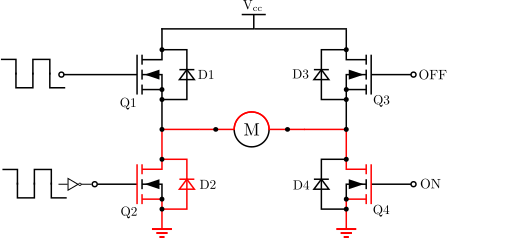
\includegraphics[scale=.6]{figures/HbridgeClockwiseBrakeOFF.pdf}
  			\centering
  			\vspace{-.4cm}
  			\captionsetup{justification=centering}
  			\captionof{figure}{Clockwise brake in off-state.\\ \emph{Edited from image by Biezl}.\cite{Biezl}}
  			\label{HbridgeClockwiseBrakeOFF}
  		\end{figure}\vspace{-5mm}
  	\end{minipage}
  \end{minipage}

There multiple ways to configure an electrical break operation of an H-bridge, in this example the PWM signal is imposed on Q2, rather than only using the intrinsic diode, D2, when in OFF-state, \figref{HbridgeClockwiseBrakeOFF} \cite{DCook}. This method creates less heat dissipation in the FET, however weather it is necessary depends largely on the specifications of the FETs and the current draw of the load.

\subsection{Double H-bridge Brake Mode}
Implemented on the vehicle is a double H-bridge, which is configured to run in brake mode as illustrated on \figref{DoubleHbridgeBrakeON} and \figref{DoubleHbridgeBrakeOFF}. 

\begin{figure}[H]
	\centering
	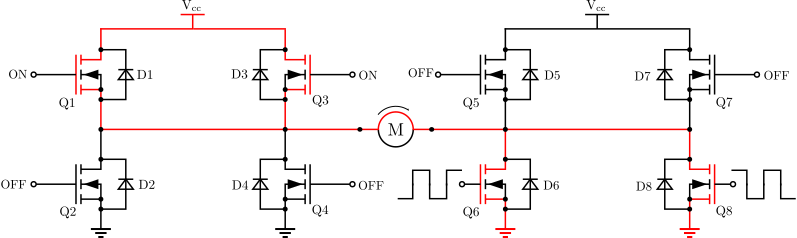
\includegraphics[scale=.6]{figures/DoubleHbridgeBrakeON.pdf}
	\caption{Double H-bridge brake operation in on-state.\\ \emph{Edited from image by Biezl}.\cite{Biezl}}
	\label{DoubleHbridgeBrakeON}
\end{figure}\vspace{-5mm}

In this configuration the PWM signal is only imposed on Q6 and Q8. So instead of activating Q5 and Q7 in the OFF-period, as in \figref{HbridgeClockwiseBrakeOFF}, it utilizes the intrinsic diodes of Q5 and Q7, as shown on \figurename{DoubleHbridgeBrakeOFF}. This can sometimes cause too high heat dissipation in the intrinsic diodes, however this H-bridge has an absolute maximum rating of \si{\pm 30 \ A}, and in this configuration has two FETs in parallel, which is more than sufficient\cite{STMicroelectronics}.

\begin{figure}[H]
	\centering
	\includegraphics[scale=.6]{figures/DoubleHbridgeBrakeOFF.pdf}
	\caption{Double H-bridge brake operation in off-state.\\ \emph{Edited from image by Biezl}.\cite{Biezl}}
	\label{DoubleHbridgeBrakeOFF}
\end{figure}\vspace{-5mm}

In brake operation the motor breaks in the OFF-period, as opposed to coast operation, where the motor runs freely in the OFF-period of the PWM signal. Though the coast mode is more energy efficient, it is harder to control the vehicle when trying to compensate for too high speeds. An H-bridge in coast operation can add more inertia to the system, however it is not very efficient when the system gains too much inertia, e.g. when going downhill. Break operation on the other hand is less energy efficient, as it dissipates to break in the OFF-period of the PWM. This however allows the H-bridge to both increase and decrease speed, which allows for better control when for instance the vehicle is going downhill.

%---------- Chapter 5 ---------------------------------------- Modelling of the Vehicle
\chapter{Modeling of the Vehicle}\label{cha:ModelOfVehicle}

The prototype model contains software, hardware and mechanical components. Software and hardware components are easy to change and to model after how the rest of the system is made and shall run. The vehicle, which is a mechanical plant, is provided to this project and therefore not changeable. This means that requirements about how the system should react, described in \secref{sec:Vehicledescription}, apply only for elements of the system that are external to the plant. In this chapter, a model of the vehicle is made to describe the power transfer from both the motor's and servomotor's rotational energy to the movement of the vehicle. Once, this model is established, it is possible to measure its output and apply a control on it, see \chapref{cha:ControlOfTheVehicle}.


\begin{figure}[H]
	\centering
	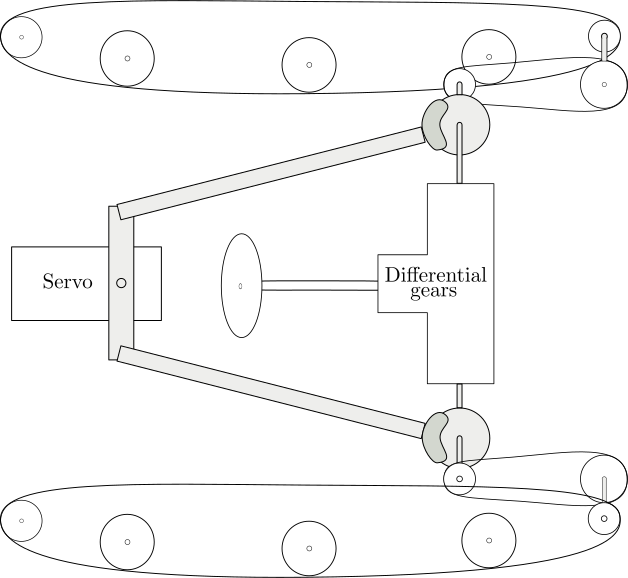
\includegraphics[scale=0.6]{figures/completeMechanical.pdf}
	\caption{A mechanical diagram of the vehicle}
	\label{fig:completeMechanicalDiagram}
\end{figure}

The \figref{fig:completeMechanicalDiagram} shows both the drivetrain and steering mechanisms on the given vehicle. It is possible to identify and separate these two sub-systems. The driving part allows the vehicle to run and comprises the motor, all the gears that make the belts turn and the belts themselves. On the other hand, the steering part is made of the servomotor which acts on two shafts and breaks one or the other belt, as stated in \secref{sec:Vehicledescription}. In the next sections, the drivetrain, which allows the vehicle to run, and the steering part, which allows the vehicle to turn, are modelled separately, and eventually recombined into a single model.
\section{Velocity Model of the Vehicle}
In this section the \textit{Vehicle} block in \chapref{cha:ModelOfVehicle} \figref{fig:StartTotalModelsystem} is opened up and modelled regarding the velocity of the vehicle. In \figref{fig:Velocitymodelplantopen} the opening of the \textit{Vehicle} block is illustrated.

\begin{figure}[H]
	\centering
	\includegraphics[scale=0.6]{figures/plantopen.pdf}
	\caption{The \textit{Vehicle} block in \chapref{cha:ModelOfVehicle} \figref{fig:StartTotalModelsystem} is opened up and illustrated in more detail}
	\label{fig:Velocitymodelplantopen}
\end{figure}

The velocity model of the \textit{vehicle} has been split up into a motor and a drivetrain section. The motor receives an input from the controller regulating its supplied voltage. the motor then delivers a rotational force as an output to the drivetrain. The drivetrain then generates the actual speed as the output of the \textit{Vehicle} block. as well as supplying the motor with an angular velocity which is dependent on the total inertia of the system, and thereby insures that the motor is affected by its load. The two sections, the motor and drivetrain, is generated by only considering the parameters affecting the vehicle when the vehicle is driving in a straight line. Thus, excluding the differential steering and thereby only modelling the system when the wheels have the exactly same velocity.

In the following subsection the motor will be modelled.
\subsection{Motor modelling}
A model of a motor consist of both a mechanical and an electrical section, due to the electrical current, $i_a(t)$, converting into a rotational force called torque, $\tau_m$. Therefore a model of the mechanical and the electrical system is produced. The electrical model provides the motors torque and the mechanical model from the motor provides what contributions the motor delivers to the drivetrain, see \secref{DriveTrain}.

\subsubsection{Electrical model}
The output from the motors electrical model is torque, $\tau_m$. To obtain the torque, the formula for translating the electrical current, $i_a$, to torque is utilized:

\begin{flalign}\centering
  \tau_m(t) = K_t \cdot i_a(t) %\unit{\volt}
  \label{equ:motortorque}
\end{flalign}
\hspace{6mm} Where:\\
\begin{tabular}{p{1cm}ll}
& $\tau_m$ & is the rotational force torque [$N \cdot m$] \\
& $i_a(t)$ & is the electrical closed loop current [$A$]\\
& $K_t$ & is the torque constant [$\frac{N \cdot m}{A}$] \\
\end{tabular}

An expression for the current, $i_a$, is required to derive a model for the electrical system. In \figref{fig:electricaldiagrammotor} an electrical diagram of the motor is displayed.

\begin{figure}[H]
\centering
	\begin{circuitikz}[american voltages]
		\draw
		
		% electromotive force 
		(0,0) to [short] (6,0)
		%to [sV, l=$e_b$] (6,2) %  voltage
		(6,0) to [V, l=$e_b$] (6,3)
		%to node[short]{}(6,2)

		%to node[short]{}(0,0)		 
		(0,0) to [V, l=$V_m$] (0,3) %  voltage

		
		%to [R, l=$Z_G$] (3,3) % generator impedance
		
		(0,3) to [R, l_=$R_a$, i>_=$i_a$] (3,3)	
		
		to [L, l_=$L_a$] (6,3); 
	\end{circuitikz}
  \caption{A electrical diagram of the motor}
  \label{fig:electricaldiagrammotor}
\end{figure}

By using Kirchoffs voltage law on the closed loop, seen in \figref{fig:MotorElectric}, an expression including $i_a$ can be derived:

\begin{flalign}\centering
V_a(t) = R_a \cdot i_a(t) + L_a \cdot \frac{di_a}{dt} + e_b 
\label{MotorClosedLoop}
\end{flalign}
\hspace{6mm} Where:\\
\begin{tabular}{p{1cm}ll}
& $V_a(t)$ & is the supply voltage [$V$] \\
& $R_a$ & is the internal resistance in the motor [$\Omega$]\\
& $L_a$ & is the inductance in the motor [$H$] \\
& $e_b$ & is the electromotive force, also called EMF [$\V$] \\
\end{tabular}

The electromotive force, $e_b$, is equivalent to:

\begin{flalign}\centering
e_b = K_e \cdot \dot{\theta}_m(t) 
\end{flalign}
\hspace{6mm} Where:\\
\begin{tabular}{p{1cm}ll}
& $K_e$ & is the electromotive constant [$Wb$] \\
& $\dot{\theta}_m$ & is the angular velocity in the motor [$\frac{rad}{s}$] \\
\end{tabular}

The equivalent for the electromotive force is substituted into \eqref{MotorClosedLoop}.

\begin{flalign}\centering
V_a(t) = R_a \cdot i_a(t) + L_a \cdot \frac{di_a}{dt} + K_e \cdot \dot{\theta}_m(t)
\end{flalign}

The Laplace transform is applied to the derived equation:

\begin{flalign}\centering
V_a(s) = R_a \cdot i_a(s) + L_a \cdot s \cdot i_a(s) + K_e \cdot \omega_m(s) 
\end{flalign}

The equation is solved for $i_a$:

\begin{flalign}\centering
i_a(s) = \frac{V_a(s) - K_e \cdot \omega_m(s)}{sL_a + R_a} 
\end{flalign}

By substituting the derived equation for $i_a$ into \eqref{equ:motortorque}, a new expression for the motors torque is derived. 

\begin{flalign}\centering
  \tau_m = K_t \cdot i_a(s) = K_t \cdot \frac{V_a(s) - K_e \cdot \omega_m(s)}{sL_a + R_a}  %\unit{\volt}
  \label{eq:Totaltorquewithcurrentexpression}
\end{flalign}

A equation for the electrical model relative to the motors torque has been derived.

\subsubsection{Mechanical model}
A mechanical model is formed to analyse the forces and moments affecting the mechanical system, and to see how the system reacts to stimuli.

Newtons second law of motion for rotational systems yields:

\begin{flalign}\centering
\tau_m(t) = J_m \cdot \ddot{\theta}_m(t)
\label{eq:mechanicalmodel}
\end{flalign}
\hspace{6mm} Where:\\
\begin{tabular}{p{1cm}ll}
& $J_m$ & is the motors inertia [$kg*m^2 $] \\
& $\ddot{\theta}_m$ & is the angular acceleration in the motor [$\frac{rad}{s^2}$] \\
\end{tabular}

This law is applied to the mechanical model and visualized in \figref{fig:MotorMechanicalModel}. Furthermore it is necessary to consider the friction affecting the rotation of the motor when it is spinning. The friction is in the opposite direction of the applied rotational force torque, see \figref{fig:MotorMechanicalModel}.

\begin{figure}[H]
	\centering
	\includegraphics[scale=0.8]{figures/MotorMechanicalModel.pdf}
	\caption{A free body diagram of the motor}
	\label{fig:MotorMechanicalModel}
\end{figure}

From the figure an equation for the mechanical model can be derived.

\begin{flalign}\centering
\tau_m(t) = J_m \cdot \ddot{\theta}_m(t) + B \cdot \dot{\theta}_m(t)
\end{flalign}

The equation is transferred into the frequency domain using the Laplace transform: 

\begin{flalign}\centering
\tau(s) = J_m(s) \cdot \omega \cdot s + B \cdot \omega_m
\label{eq:ThetadotforBlock}
\end{flalign}

The mechanical model of the motor has be derived. Next step is to make block representation of the system. 

\subsubsection{Block representation}

\eqref{eq:Totaltorquewithcurrentexpression} delivers the information needed to make a visual representation of the motor model. The input is the supply voltage, $V_a(s)$ delivered to the motor and the output is the required torque, $\tau_m$, see \figref{fig:motormodelBlock}. The block representation of the system can be used, when the system is to be simulated.

\begin{figure}[H]
	\centering
	\includegraphics[scale=0.9]{figures/motormodelBlock.pdf}
	\caption{A block representation of the motor, with a voltage, $V_m(s)$, as the input and a rotational force, $\tau_m(s)$, as the output.}
	\label{fig:motormodelBlock}
\end{figure}

The angular velocity received is dependent on the total inertia of the system, and is necessary to insure the motor is affect by the load.

A model of the electrical and mechanical part has been formed and a block representation of the motors applied voltage and generated torque has been given. Next step is to model the drivetrain, which connects to the motor through the motor shaft.
\subsection{Drivetrain}\label{Drivetrain}

%% INTRODUCTION %%
The drivetrain translates the torque $\tau_m$, given by the motor, into the actual movement of the vehicle. The model of the drivetrain illustrates the relation between the applied torque, $\tau_m$, and the velocity of the vehicle. The velocity model of the drivetrain is created by only considering when the vehicle's trajectory follows a straight line.\\\\
%
The modelling of the drivetrain is limited to only model parts of the total drivetrain system, to make it more manageable and with a focus on giving a rough approximation.
%% SSSECTION : BLACK BOX MODEL %%
\subsubsection{Black Box Model}\label{BlackBoxModel}
To get a rough approximation of how the drivetrain works, a blackboxed model is used. The blackbox in the model is placed between box 1 and box 4 seen in \chapref{VehicleDescription} \figref{vehicleDescriptionDriveTrain}. The gear, $G_m$, connected to the motor shaft, is connected to the gear ,$G_d$, which represents the gears and shaft that has been black boxed and the drive-wheel, see \figref{fig:DrivetrainMechanicalModel}. The number of teeth on the gear, $G_d$, is set to the total gear ratio of the black box.

\begin{figure}[H]
	\centering
	\includegraphics[scale=0.8]{figures/mechanicalDrawingSystem.pdf}
	\caption{A rough mechanical diagram of the drivetrain}
	\label{fig:DrivetrainMechanicalModel}
\end{figure}
\todo{Add notations to the diagram and create free body diagrams of belt and black box parts}

% APPLICATION OF NEWTON'S SECOND LAW %

\begin{figure}[H]
	\centering
	\includegraphics[scale=0.8]{figures/freeBodyMotorGear.pdf}
	\caption{A free body diagram of the motor gear}
	\label{fig:MotorGearFreeBodyDiagram}
\end{figure}

\begin{figure}[H]
	\centering
	\includegraphics[scale=0.8]{figures/freeBodyDrive.pdf}
	\caption{A free body diagram of the `black box' gear}
	\label{fig:BlackBoxGearFreeBodyDiagram}
\end{figure}

The \eqref{eq:mechaUnloadedMotor} is extended with the contribution of the load which is the whole drivetrain. Therefore, from \figref{fig:MotorGearFreeBodyDiagram} and Newton's second law appplied to rotational systems, the following equation can be extracted:
\begin{flalign}\centering
J_m \cdot \dot{\omega}_m(t) = \tau_m(t) - B_m \cdot \omega_m(t) - N_m \cdot f_c(t) 
\label{eq:MotorGearNewtonSecLaw}
\end{flalign}
\hspace{6mm} Where:\\
\begin{tabular}{p{1cm}ll}
& $J_m$ 			      & is the motor's inertia [$kg \cdot m^2$] \\
& $\omega_m$        & is the angular velocity of the motor [$rad \cdot s^{-1}$] \\
& $\dot{\omega}_m$ 	& is the angular acceleration of the motor [$rad \cdot s^{-2}$] \\
& $\tau_m$ 		     	& is the torque delivered by the motor [$N \cdot m$] \\
& $B_m$             & is the coefficient of the friction happening inside the motor [$N \cdot m \cdot s \cdot rad^{-1}$] \\
& $N_m$             & is the number of teeth of the motor gear $G_m$ [$number\ of\ teeths$] \\
& $f_c$             & is the coefficient of the contact force between $G_m$ and $G_d$ [$N \cdot m \cdot number\ of\ teeths^{-1}$]
\end{tabular}

The equation for \figref{fig:BlackBoxGearFreeBodyDiagram} is obtained the same way:
\begin{flalign}\centering
J_d \cdot \dot{\omega}_d(t) = N_d \cdot f_c(t) - N_d \cdot f_b(t)
\label{eq:BlackBoxGearNewtonSecLaw}
\end{flalign}
\hspace{6mm} Where:\\
\begin{tabular}{p{1cm}ll}
& $J_d$ 			      & is the `black box' gear inertia [$kg \cdot m^2$] \\
& $\omega_d$        & is the angular velocity of the `black box' gear [$rad \cdot s^{-1}$] \\
& $\dot{\omega}_d$ 	& is the angular acceleration of the `black box' gear [$rad \cdot s^{-2}$] \\
& $N_d$ 		     		& is the number of teeth on the `black box' gear [$number\ of\ teeth$] \\
& $f_b$             & is the coefficient of the contact force between $G_d$ and the belt [$N \cdot m \cdot number\ of\ teeths^{-1}$] \\
\end{tabular}

%% SSSECTION : BELT MODEL %%
\subsubsection{Belt Model}\label{BeltModel}

\begin{figure}[H]
	\centering
	\includegraphics[scale=0.8]{figures/mechanicalDrawingBelt.pdf}
	\caption{A mechanical diagram of the belt part}
	\label{fig:BeltMechanicalDiagram}
\end{figure}

\begin{figure}[H]
	\centering
	\includegraphics[scale=0.8]{figures/freeBodyBelt.pdf}
	\caption{A free body diagram of the belt driven mass}
	\label{fig:BeltFreeBodyDiagram}
\end{figure}

From \figref{fig:BeltFreeBodyDiagram}, the mechanical equation of the belt system on \figref{fig:BeltFreeBodyDiagram} is found to be:
\begin{flalign}\centering
M \cdot \dot{v}(t) = r_t \cdot f_b(t) - B_{sys} \cdot v(t)
\label{eq:BeltMassNewtonSecLaw}
\end{flalign}
\hspace{6mm} Where:\\
\begin{tabular}{p{1cm}ll}
& $M$ 			  & is the vehicle's total weight [$kg$] \\
& $v$        	& is the linear velocity of the behicle [$m \cdot s^{-1}$] \\
& $\dot{v}$ 	& is the linear acceleration of the vehicle [$m \cdot s^{-2}$] \\
& $r_t$ 		  & is the translational coefficient between the last gear and the belt [$m \cdot number\ of\ teeths^{-1}$] \\
& $B_{sys}$   & is the coefficient of the friction happening throughout the gears [$N \cdot s \cdot rad^{-1}$] \\
\end{tabular}

The assembling of a model for the drivetrain is made from these separate mechanical equations.

% SSSECTION : ASSEMBLING OF THE DIFFERENT EQUATIONS %
\subsubsection{Drivetrain modeling}\label{DrivetrainModeling}
The combination of \eqref{eq:MotorGearNewtonSecLaw}, \eqref{eq:BlackBoxGearNewtonSecLaw} and \eqref{eq:BeltMassNewtonSecLaw} makes it possible to get the linear velocity of the vehicle $v$ out of the torque $\tau_m$ given by the motor. Indeed, it is possible to link these equations throughout the contact force coefficients $f_c$ and $f_b$.\\\\
%
Taking the Laplace-transform of these equations helps arranging them and eventually, to find a transfer function from $\tau_m(s)$ to $V(s)$ :
%
\begin{flalign}\centering
J_m \cdot s \cdot \omega_m(s) = \tau_m(s) - B_m \cdot \omega_m(s) - N_m \cdot F_c(s) 
\label{eq:MotorGearNewtonSecLawLaplace}
\end{flalign}
%
\begin{flalign}\centering
J_d \cdot s \cdot \omega_d(s) = N_d \cdot F_c(s) - N_d \cdot F_b(s)
\label{eq:BlackBoxGearNewtonSecLawLaplace}
\end{flalign}
%
\begin{flalign}\centering
M \cdot s \cdot V(s) = r_t \cdot F_b(s) - B_{sys} \cdot V(s)
\label{eq:BeltMassNewtonSecLawLaplace}
\end{flalign}
%
By finding the expressions for $F_b$ from \eqref{eq:BeltMassNewtonSecLawLaplace} and then $F_c$ from \eqref{eq:BlackBoxGearNewtonSecLawLaplace}, it is then possible to insert $F_b$ expression into $F_c$'s and the latter into \eqref{eq:MotorGearNewtonSecLawLaplace}.
%
\begin{flalign}\centering
r_t \cdot F_b(s) =  M \cdot s \cdot V(s) - B_{sys} \cdot V(s) 
\label{eq:BeltContactForceLaplace}
\end{flalign} \todo{Get the second implication to be on the next line}
%
\begin{flalign}\centering
F_b(s) =  \frac{M \cdot s \cdot V(s) - B_{sys} \cdot V(s)}{r_t}
\label{eq:BeltContactForceLaplace}
\end{flalign} \todo{Get the second implication to be on the next line}

And $F_c$ is found this way from \eqref{eq:BlackBoxGearNewtonSecLawLaplace}:
\begin{flalign}\centering
N_d \cdot F_c(s) = J_d \cdot s \cdot \omega_d(s) + N_d \cdot F_b(s) 
\end{flalign}
\begin{flalign}\centering
F_c(s) =  \frac{J_d \cdot s \cdot \omega_d(s) + N_d \cdot F_b(s)}{N_d} =  \frac{J_d \cdot s}{N_d} \cdot \omega_d(s) + F_b(s)
\label{eq:GearsContactForceLaplace}
\end{flalign}

\todo{Get the steps to be on different lines}
%
Moreover, the relation of velocity for two gears $G_m$ and $G_d$ in contact is given by:
\begin{flalign}\centering
N_m \cdot \omega_m = N_d \cdot \omega_d, 
\label{eq:GearsVelocityRelation}
\end{flalign}

which is equivalent to :
\begin{flalign}\centering
\omega_m = \frac{N_d}{N_m} \cdot \omega_d \xRightarrow{\mathcal{L}} \omega_m(s) = \frac{N_d}{N_m} \cdot \omega_d(s).
\label{eq:BlackBoxGearNewtonSecLaw}
\end{flalign}
%
The same principle is applied from the angular velocity $\omega_d$ to the translational velocity $V$:
\begin{flalign}\centering
v(t) = r_t \cdot \omega_d(t) = r_t \cdot \frac{N_m}{N_d} \cdot \omega_m(t) \xRightarrow{} \omega_m(t) = \frac{N_d}{N_m \cdot r_t} \cdot v(t)
\label{eq:BlackBoxGearNewtonLaplaceNew}
\end{flalign}
Again, the Laplace transform is used to manipulate equations more easily:
\begin{flalign}\centering
\omega_m(s) = \frac{N_d}{N_m \cdot r_t} \cdot V(s).
\label{eq:BlackBoxGearNewtonLaplaceNew}
\end{flalign}

It is now possible to replace $\omega_d$ and $F_b$ in \eqref{eq:GearsContactForceLaplace}:
\begin{flalign}\centering
F_c(s) =  \frac{J_d \cdot s}{N_d} \cdot \frac{1}{r_t} \cdot V(s) + V(s) \cdot \left[\frac{M \cdot s + B_{sys}}{r_t}\right] = V(s) \cdot \left[\frac{J_d \cdot s}{r_t \cdot N_d} + \frac{M \cdot s + B_{sys}}{r_t} \right].
\label{eq:GearsContactForceLaplaceNew}
\end{flalign}

And the desired relation between the motor torque and the linear velocity is finally obtained :
\begin{flalign}\centering
\tau_m(s) = J_m \cdot \frac{N_d}{N_m \cdot r_t} \cdot V(s) \cdot s + B_m \cdot \frac{N_d}{N_m \cdot r_t} \cdot V(s) + N_m \cdot \left[\frac{J_d \cdot s}{r_t \cdot N_d} + \frac{M \cdot s + B_{sys}}{r_t} \right] \cdot V(s) = V(s) \cdot \frac{1}{r_t} \cdot \left[\frac{J_m \cdot N_d}{N_m} \cdot s + N_m \cdot J_d \cdot s + M \cdot s + N_m \cdot B_{sys} + B_m \cdot \frac{N_d}{N_m} \right]
\end{flalign}

Therefore, the transfer function from $\tau_m$ to $V$ is :
\begin{flalign}\centering
\frac{V(s)}{\tau_m(s)} = \frac{r_t}{\left[\frac{J_m \cdot N_d}{N_m} + N_m \cdot J_d + M\right] \cdot s + \left[B_{sys} \cdot N_m + B_m \cdot \frac{N_d}{N_m} \right]}
\label{eq:TransferFunctionTorqueToVelocity}
\end{flalign}

Eventually, it is possible to draw a block diagram for the drivetrain, from the motor torque to the vehicle's velocity with \eqref{eq:TransferFunctionTorqueToVelocity} and also back to the angular velocity with \eqref{eq:BlackBoxGearNewtonLaplaceNew}, see \figref{fig:BeltFreeBodyDiagram}.

\begin{figure}[H]
	\centering
	\includegraphics[scale=0.8]{figures/blockDiagramDrivetrain.pdf}
	\caption{A block diagram of the drivetrain}
	\label{fig:BlockDiagramDrivetrain}
\end{figure}

\section{Final Velocity Model}
\eqref{eq:Totaltorquewithcurrentexpression} delivers the information needed to make a visual representation of the motor model. The input is the supply voltage, \si{V_m(s)} delivered to the motor and the output is the required torque, \si{\tau_m}, see \figref{fig:BlockDiagramDrivetrain}. The block representation of the system is used, when the system is to be simulated.

\begin{figure}[H]
	\centering
	\includegraphics[width=\textwidth]{figures/totalVelocityModelDiagramComplicated.pdf}
	\caption{A block diagram of the combined drivetrain}
	\label{fig:BlockDiagramDrivetrain}
\end{figure}

The angular velocity received from the drivetrain, see \figref{fig:Velocitymodelplantopen}, is dependent on the total inertia of the system, and is necessary to ensure the motor is affected by the load.

A model of the electrical and mechanical part has been formed and a block representation of the motor's applied voltage and generated torque has been given. Next step is to model the drivetrain, which connects to the motor through the motor shaft.
\subsection{Simulation and Simplified Model}
The previous sections show a velocity model of the system which is modelled in this section. As mentioned in the inertia test, \appref{app:inertiaTest}, the armature inductance is so small that it is not necessary to include for a good simulation. If the armature inductance is neglectable, and removed, the system will appear as a first order system instead of a second order. Therefore \si{L_a} is set to zero and hence removing the second order term. This effect is illustrated in the transfer function:
%
\begin{flalign}
  \eq{\frac{V(s)}{U_a(s)}}{ \frac{K_t}{L_a \cdot J_{tot} \cdot s^2 + (R_a \cdot J_{tot} + L_a \cdot B_{tot}) \cdot s + R_a \cdot B_{tot} + K_t \cdot K_e }}\nonumber\\
  &\Downarrow&\nonumber\\
  \eq{\frac{V(s)}{U_a(s)}}{ \frac{ K_t }{ R_a \cdot J_{tot}  \cdot s + R_a \cdot B_{tot} + K_t \cdot K_e }}\nonumber\\
  \eq{\frac{V(s)}{U_a(s)}}{ \frac{ \frac{K_t}{R_a \cdot B_{tot} + K_t\cdot K_e} }{ \frac{R_a \cdot J_{tot}}{R_a \cdot B_{tot} + K_t \cdot K_e}\cdot s + 1 }}
  \label{eq:simplifiedTransferVel}
\end{flalign}
%
By inspection of the first order expression, in \eqref{eq:simplifiedTransferVel}, the terms for the time constant and the gain are extracted:
\begin{flalign}
  \eq{K}{\frac{K_t}{R_a \cdot B_{tot} + K_t\cdot K_e}}&\nonumber\\
  \eq{\tau }{ \frac{R_a \cdot J}{R_a \cdot B_{tot} + K_t \cdot K_e} }\nonumber&
\end{flalign}
%
To verify that this is a viable approximation, the following simplified model, in \figref{fig:BlockDiagramDrivetrainSimplified}, is created:
%
\begin{figure}[H]
	\centering
	\includegraphics[scale = .5]{figures/totalVelocityModelDiagramSimplified.pdf}
	\caption{A block diagram showing a simplified model}
	\label{fig:BlockDiagramDrivetrainSimplified}
\end{figure}
%
Where \si{K} is the gain of the system and \si{\tau} is the time constant. This simplified first order model of the system is simulated alongside the second order model, to verify that the vehicle can indeed be handled as a first order system. The plot of the two simulations are illustrated in \figref{fig:ComparisonOf1stAnd2ndOrderModels}.
%
From this figure it is impossible to see any difference between the two models, however, zooming in on the base of the step, see \figref{fig:comparison1stAnd2ndOrderModelsZoom}, the difference becomes clear.
%
\begin{minipage}{\linewidth}
  	\centering
  	\begin{minipage}{0.45\linewidth}
  		\begin{figure}[H]
  			\centering
  			\includegraphics[scale = .6]{figures/ComparisonOf1stAnd2ndOrderModels.png}
  			\caption{Comparison of the \si{1^{st}} and \si{2^{nd}} order models}
  			\label{fig:ComparisonOf1stAnd2ndOrderModels}
  		\end{figure}
  	\end{minipage}
  	\hspace{0.03\linewidth}
  	\begin{minipage}{0.45\linewidth}
  	  \begin{figure}[H]
    	 	\centering
    	 	\includegraphics[scale = .6]{figures/comparison1stAnd2ndOrderModelsZoom.png}
    	 	\caption{Comparison of the \si{1^{st}} and \si{2^{nd}} order models}
    	 	\label{fig:comparison1stAnd2ndOrderModelsZoom}
    	\end{figure}
  	\end{minipage}
  \end{minipage}

However, a quick glance at the axes shows how minimal the impact of this difference must be. An other and possibly clearer way to show the difference of the two models, is through use of Bode plots. A Bode plot of the two models imposed on one another is seen on \figref{bodePlotOf1stAnd2ndOrderModel}.
%
\begin{figure}[H]
	\centering
	\includegraphics[width = \textwidth]{figures/bodePlotOf1stAnd2ndOrderModel.png}
	\caption{Bode plot showing the differences between the \si{1^{st}} and \si{2^{nd}} order models}
	\label{fig:bodePlotOf1stAnd2ndOrderModel}
\end{figure}
%
For frequencies below 1000 \si{rad\cdot s^{-1}} the two models are very similar because each of their first poles are very close; in 3,8759 \si{rad\cdot s^{-1}} for the \si{1^{st}} order model and 3,9 \si{rad\cdot s^{-1}} for the \si{2^{nd}} order model. The \si{2^{nd}} order model however has an other pole which causes the phase shift and shift in magnitude at higher frequencies. However since this pole is so high, 1489,5 \si{rad\cdot s^{-1}}, it does not affect the lower pole considerably and the differences are way beyond significant frequency range.

In the following section the simplified model is verified directly by comparison with recorded data of the vehicle's step response.
\subsection{Linear Approximation}
And theeeeeeeeeeeeeeeeeeeeen???
\subsection{Verification of the Velocity Model}
In the former section a simplified first order model of the vehicle's velocity model was established. To ensure the approximation is a reliable model of the system, it is compared to a measured step-response of the vehicle. However, the simulation uses a first order model as described in the previous section, the gain, found in \appref{app:gainTest} and the time constant, found in \appref{app:inertiaTest}, is used as the first orders parameters. In \figref{SimulationIRLsteprespons2} the simulated model's step-response and the measured step-response of the vehicle is illustrated. 
%
\begin{figure}[H]
  \centering
 	%Trim margins @:   left        bottom       right       top
 	\adjustbox{ trim = {.15\width} {.30\height} {.15\width} {.30\height}, clip }
  {
    \includegraphics[width=1.4\textwidth]{figures/SimulationIRLsteprespons2.pdf}
  }
  \caption{A plot illustrating a simulated step-response of the approximated velocity model (the blue line) and a measured step-response of the vehicle (the red line).}
  \label{SimulationIRLsteprespons2}
\end{figure}
%
In \figref{SimulationIRLsteprespons2} the red line is the measured data from the vehicle's step-response. To ensure enough data points is registered by the Hall sensor, when performing the step-response of the vehicle, the vehicle is set to drive at \si{1\ m\cdot s^{-1}} at the start of the test. The vehicle preserves this velocity continuously for three seconds, before the vehicle is set to drive at its maximum velocity. The simulation (the blue line) is set to have the same milestones as the measured step-response of the vehicle. Furthermore it can be seen in \figref{SimulationIRLsteprespons2} that the simulation starts before zero, this is due to rounding errors in simulated transfer-function, which is disregarded.

The occurrence of stiction in the start of the simulation and measured step-response, has been eliminated to a certain extent, which makes it insignificant. Furthermore, even though the vehicle is moving at a velocity of $0$ \si{m \cdot s^{-1}}, the velocity is registered to be $0,04$ \si{m \cdot s^{-1}}, see why in \secref{sec:hallFiltering}. 

The little bump in the beginning of the measured step-response, the red line, is caused by the lag of the Hall sensors. This is, however, disregarded. Additionally, the ripples seen on the measured step-response, when the vehicle is at its maximum velocity, could be caused by different kinds of noise factors, e.g:

\begin{itemize}
\item Uneven belts
\item Uneven floor
\item Belts slipping on the floor
\item Wear and tear on the internal gears
\end{itemize}

The data from the simulated and measured step-response illustrated in \figref{SimulationIRLsteprespons2}, when compared is very similar, except for the bump and ripple on the measured data. Besides these two elements the approximated velocity model is sufficient.
\section{Steering Model of the Vehicle}\label{sec:SteeringModel}
\todo{rewrite}The following section will describe and model the steering of the vehicle. The relationship between the vehicle's speed, the angle of the servo, the brakes, and the actual steering of the vehicle will be examined. A overview of the braking system can be seen in \figref{steeringMechanical}.

 \begin{figure}[H]
 	\centering
 	\includegraphics[scale=0.6]{figures/steeringMechanical.pdf}
 	\caption{Mechanical drawing of the steering}
 	\label{steeringMechanical}
 \end{figure}

When the servo turns one way, it push the brake pads on the brake disc, to add a friction. The differential gears will transfer the power from one belt to the other if one brake is triggered.

\subsection{Steering Parameters}
As the steering system contains many moving parts, it would be advantageous to start with a simple model, verifying it, and iterate until it is satisfactory. 

The first model considered can be seen on \figref{basicSteering}.

\begin{figure}[H]
	\centering
	\includegraphics[width=0.8\textwidth]{figures/basic_steering_model.jpg}
	\caption{A basic steering model}
	\label{basicSteering}
\end{figure}
 
As described in \secref{Servo}, the angle of the servo is proportional to a pulse width modulated signal on it's control input. The pulse width is therefore chosen as the input in this model. This is multiplied by a constant, $\text{K}_\text{s}$, which translates the pulse width to an angle of the servo.
If the velocity of the vehicle is assumed constant, the rate of change of the direction must be a function of the servo angle, and a constant, $\text{K}_\text{c}$, representing the speed of the vehicle.
The rate of change is integrated over time, resulting in a direction. 

As the vehicle has to follow a predetermined route, a direction alone is not enough. As seen on \figref{SteeringDeviation}, any change of direction caused by a disturbance, will cause a deviation from the planned line from A to B.

\begin{figure}[H]
	\centering
	\includegraphics[width=0.8\textwidth]{figures/steering_deviation.jpg}
	\caption{Consequence of using directional control alone}
	\label{SteeringDeviation}
\end{figure}

How large the deviation will be must depend on the erroneous angle, the speed, and the time it takes to correct the error. Assuming the speed is constant, the error can be described as an integration of the error angle over time.


Second or first order, if it is second the black box should be expanded, if it is first there is no need because then we have all the parameters from the test.
 
\begin{figure}[H]
	\centering
	\includegraphics[scale=1]{figures/steeringDiagramBlackBox.pdf}
	\caption{A diagram showing the black box}
	\label{steeringDiagramBlackBox}
\end{figure}
 
%  appendix
 
% show that it's a first order system\\
% then integrator\\
% then is linear(multiples values) the speed of turning at different PWM angle of the servo?


%---------- Chapter 6 ---------------------------------------- Control of the vehicle
\chapter{Control of the Vehicle}\label{cha:ControlOfTheVehicle}
%Sources used in this section:
%\cite{WSLevine}
%\cite{BatteryDS}
%\cite{BGLiptak}
%\cite{KJAAstrom}

\section{Velocity Controller}\label{sec:velocityController}
The purpose of the velocity controller is to preserve the vehicle at a steady velocity, when going uphill, downhill and when turning, this is in conjunction with the velocity requirement from \secref{Requirements}. The three most widely utilized controllers are the proportional, integral and differential controllers\cite{WSLevine}. Usually all three controllers combined are not required when controlling a system. Different controller approaches are explored in the following segment, starting with the controller which is the most frequently utilized controller, alone or in combination with others, the proportional controller.

\subsection{P-Controller}
As illustrated on \figref{proportionalController} the P-controller, \si{K_p}, is a proportional gain which is multiplied with the direct term.
%
\begin{figure}[H]
 	\centering
 	\includegraphics[scale=0.6]{figures/proportionalController.pdf}
 	\caption{Diagram of the proportional controller}
  \label{proportionalController}
\end{figure}

The illustrated diagram yields the following closed loop transfer function:
%
\begin{flalign}
  \eq{ \frac{V_{out}}{V_{ref}} }{\frac{\frac{K_p \cdot K}{\tau \cdot s +1}}{1 + \frac{K_p \cdot K}{\tau \cdot s +1}} = \frac{1}{ \frac{ \tau \cdot s + 1 }{ K_p \cdot K + 1 } + 1} = \frac{\frac{ K_p \cdot K }{ K_p \cdot K + 1 } }{ \frac{ \tau }{ K_p \cdot K + 1 } \cdot s + 1}}&
\label{eq:PclosedLoopTfs}
\end{flalign}
%
From \eqref{eq:PclosedLoopTfs} it is evident that the time constant and the gain for the system is dependent on the chosen \si{K_p}. The time constant of the closed loop transfer function is the coefficient of s in standard form:
%
\begin{flalign}
  \eq{ \tau_{closed} }{ \frac{ \tau }{ K_p \cdot K + 1 } }&\nonumber
\end{flalign}
%
As an example, the \si{K_p} is chosen such that it cancels out the gain, \si{K}, of the plant. This results in a time constant and a gain which is reduced to half:

\begin{flalign}
  \eq{ \frac{V_{out}}{V_{ref}} }{ \frac{\frac{ \frac{1}{K} \cdot K }{ \frac{1}{K} \cdot K + 1 } }{ \frac{ \tau }{ \frac{1}{K} \cdot K + 1 } \cdot s + 1} }&\nonumber\\
  \eq{ \frac{V_{out}}{V_{ref}} }{\frac{\frac{1}{2}}{\frac{\tau}{2} \cdot s + 1}}&\label{eq:PclosedLoop}
\end{flalign}
%
This results in the P-controller giving an output of half the input, but rise to its set-point twice as fast as the system step without control. This is tested utilizing the vehicle and the response is as expected. The test can be seen in \appref{app:proportionalControllerTest}.
%

If a system where an input velocity is equal to an output velocity is desired, a P-controller is insufficient. The reason lies in the numerator in \eqref{eq:PclosedLoopTfs}. No matter the value of \si{K_p} the numerator will always be less than 1. This results in an offset. A larger \si{K_p} resulting in a smaller offset, will make the coefficient of s in \eqref{eq:PclosedLoopTfs} (time constant) smaller, which can result in larger overshoot.

\subsection{P-Controller with Feed Forward}
The P-controllers difference between the reference and set-point, steady state offset, can be diminished without compromising the time constant, through use of feed forward, see \figref{proportionalControllerWithFeedforward}.\cite{KJAAstrom}
%
\begin{figure}[H]
 	\centering
 	\includegraphics[scale=0.5]{figures/proportionalControllerWithFeedforward.pdf}
 	\caption{Diagram of the proportional controller with feedforward}
 	\label{proportionalControllerWithFeedforward}
\end{figure}
%
In this design the set-point is changed by feed forwarding the desired value of the output, \si{V_{out}}, to the input of the plant. Thereby summing up the desired value with the error, \si{V_e}, fed through the P-controller. The gain located on the feed forward ensures the input, \si{V_{ref}}, has the same unit as the signal going into the plant, in the case volts, \si{U}. Since the system gain, \si{K}, converts volts into linear velocity, the gain in the forward feed is set to \si{\frac{1}{K}}. The control loop in \figref{proportionalControllerWithFeedforward} yields the following closed loop transfer function:
%
\begin{flalign}
  \eq{ \frac{V_{out} }{V_{ref}} }{ \frac{\frac{K\cdot \frac{1}{K}+K\cdot K_p}{1+K \cdot K_p}}{\frac{\tau}{1+K\cdot K_p}\cdot s + 1 } }&\nonumber
\end{flalign}
%
If the \si{K_p} value is selected to cancel out the system gain, as with the P-controller, allowing for velocity directly on the controller input, the following equation emerges from the closed loop transfer function:
%
\begin{flalign}
  \eq{ \frac{V_{out} }{V_{ref}} }{ \frac{\frac{K\cdot \frac{1}{K}+K\cdot \frac{1}{K}}{1+K \cdot \frac{1}{K}}}{\frac{\tau}{1+K\cdot \frac{1}{K}}\cdot s + 1 } }&\nonumber\\
  \eq{ \frac{V_{out} }{V_{ref}} }{ \frac{1}{\frac{\tau}{2} \cdot s + 1} }&\nonumber
\end{flalign}
%
If this is compared to the resulting closed loop transfer function for the original P-controller, \eqref{eq:PclosedLoop}, it can be seen that the steady state offset is removed. Notice that the time constant of the closed loop remains half of that of the plant. 

By utilizing the feed forward to place the set-point of the controller, P-control becomes a viable option for controlling a velocity. This is tested utilizing the vehicle and the response is as expected. The test can be seen in \appref{app:proportionalControllerTest}. A Comparing of a step response utilizing the vehicle and a simulation of a step response is illustrated in figure \figref{fig:stepPfeedForward}.
%
\begin{figure}[H]
 	\centering
 	\includegraphics[width=.9\textwidth]{figures/stepPfeedForward}
 	\caption{Proportional control with feed forward. The simulation is first order while the vehicle is second order due to the armature coils in the motor.}
 	\label{fig:stepPfeedForward}
\end{figure}
%
There are a few things to notice. First, the rise time of the two are approximately equal, however, the simulation of the first order approximation rises directly, while the measured data has a delayed initial rise. This delay is presumably because of the armature coils in the motor, through which the current cannot change instantaneously. This effect gives rise to a second order term, as discussed in \secref{DriveTrain}, where the first order approximation was made. After the armature coils have been energized the controller output has a much faster effect on the velocity of the vehicle, causing it to rise so fast that it overshoots due to inertia.

An other interesting thing to notice is the sudden drop in battery voltage. When large currents are drawn from a NiMH battery, the voltage drops\cite{BatteryDS}. However in the implementation the duty cycle is scaled according to the current battery voltage, so that the controller maintains the same effect regardless of battery voltage. The exception being when the controller output exceeds the battery voltage, in which case the control will follow the battery voltage until the battery recovers.
%
The P-controller with feed forward seems to be a good choice, however if subjected to disturbances some problems emerge. A disturbance imposed on the system is analogue to a sudden change of the gain of the plant. since the set-point compensation origins at the input of the controller, the sudden change in gain of the plant cannot be compensated for with this feed forward P-controller.
%
The effect is demonstrated in \figref{fig:hillPfeedForward}, where the feed forward controller is going up a hill.
%
\begin{figure}[H]
 	\centering
 	\includegraphics[width=.9\textwidth]{figures/hillPfeedForward}
 	\caption{When the P-controller with feed forward is subjected to constant disturbances, the gain of the system changes and the proportional gain and set-point is no longer sufficient, to avoid steady state error.}
 	\label{fig:hillPfeedForward}
\end{figure}
%
Since the vehicle steers by breaking on one side, this kind of steady state error will not only occur when encountering slopes, but every time the vehicle turns.
%
\subsection{PI-Controller} \label{sec:PIcalc}
To attack the new offset-problem caused by changes in the system gain when disturbances affects the system, a proportional integral controller is the next natural choice. The reason for choosing a PI-controller is because the I-component integrates over the error. This component therefore increases or decreases over time, and therefore has an adaptive effect on the system. The design is illustrated in \figref{proportionalIntegratorController}
%
\begin{figure}[H]
 	\centering
 	\includegraphics[scale=0.6]{figures/proportionalIntegratorController.pdf}
 	\caption{Diagram of the proportional integral controller}
 	\label{proportionalIntegratorController}
\end{figure}
%
The standard equation for a PI-controller can be rewritten to:
%
\begin{flalign}
  \eq{K_p\cdot\left(1+ \frac{1}{T_i\cdot s}\right)}{K_p \cdot \frac{T_i \cdot s + 1}{T_i \cdot s}}&\nonumber
\end{flalign}
%
Where \si{T_i} is the time constant of the integrator. Now if the time constant of the integrator is matched to the time constant of the plant, that is \si{T_i = \tau}, the following equation emerges from the closed loop transfer function:
%
\begin{flalign}
  \eq{\frac{V_{out} }{V_{ref}}}{\frac{K_p \cdot \frac{\tau \cdot s + 1}{\tau \cdot s} \cdot \frac{K}{\tau \cdot s + 1 }}{1 + K_p \cdot \frac{\tau \cdot s + 1}{\tau \cdot s} \cdot \frac{K}{\tau \cdot s + 1 }}}  \ \ \Leftrightarrow  \ \ 
  \si{\frac{V_{out} }{V_{ref}} = \frac{K_p \cdot \frac{K}{\tau \cdot s}}{1 + K_p \cdot \frac{K}{\tau \cdot s} }}&\nonumber
\end{flalign}
%
Inserting \si{K_p = \frac{1}{K}}, yields the following:
%
\begin{flalign}
  \eq{\frac{V_{out} }{V_{ref}}}{\frac{\frac{1}{K} \cdot \frac{K}{\tau \cdot s}}{1 + \frac{1}{K} \cdot \frac{K}{\tau \cdot s} }} \ \ \Leftrightarrow  \ \  \si{\frac{V_{out} }{V_{ref}} = \frac{\frac{1}{\tau \cdot s}}{1 + \frac{1}{\tau \cdot s} }} \ \ \Leftrightarrow  \ \  \si{\frac{V_{out} }{V_{ref}} = \frac{1}{\tau \cdot s + 1}}&\nonumber
 \label{eq:1overkinserted}
\end{flalign}
%
This is equivalent to the plant but with a gain of 1 instead of K, which is desirable, and so also the reason for inserting \si{K_p = \frac{1}{K}} in \eqref{eq:1overkinserted}.
Now to determine \si{K_i}, the original equation for a PI-controller is evaluated:
%
\begin{flalign}
  \si{K_p + K_i\cdot \frac{1}{s}} &= \si{K_p\cdot\left(1+ \frac{1}{T_i\cdot s}\right) \ \ \Rightarrow \ \ K_i\cdot \frac{1}{s} = \frac{K_p}{T_i\cdot s} \ \ \Rightarrow \ \ K_i = \frac{K_P}{T_i} \ \ \Rightarrow \ \ K_i = \frac{K_p}{\tau}}&\nonumber
\end{flalign}
%
This concludes the initial design of the PI-controller, however, in the following segment the controller will be analyzed and compared to the other controllers. Implementation and discussion of results follow immediately after.

\subsection{Comparison of the Controllers}
On \figref{fig:ControllerSteps} the different controller designs are simulated being subjected to a velocity step of 1.4 \si{m \cdot s^{-1}}. Furthermore, to compared the controllers with a step response of the plant, the plant is subjected to a voltage step calculated from the velocity step and the gain of the plant, corresponding to the value \si{K_p}. Since it is a step response of a plant, and not a controller, no feedback is utilized.
%
\begin{figure}[H]
 	\centering
 	\includegraphics[width=.9\textwidth]{figures/ControllerSteps}
 	\caption{Simulations of the different controller designs along with the first order system model, plant, which in this simulation has an added scale-factor to obtain a gain of 1.}
 	\label{fig:ControllerSteps}
 \end{figure}
%
A thing to notice on \figref{fig:ControllerSteps}, is the inadequacy of the P-controller, given by its steady state error. The feed forward P-controller however, solving this problem, seems like a very good solution if consulting only its step response. As discussed, a problem arises when introducing a disturbance, as seen in \figref{fig:hillPfeedForward}. The last discussed option is the PI-controller, which places itself right on top of the step response of the plant when having a gain of 1, which is by design. The difference between the plant with a scaled input to obtain a gain of 1, compared to the PI-controller lies in the feedback along with the adaptive gain emerging from the I-component. It becomes clear when investigating the open loop rather than the closed loop transfer function:
%
\begin{flalign}
  V_{error}(s) \cdot \frac{(K_p \cdot \frac{K_i}{s}) \cdot K}{\tau \cdot s + 1}
  \left.\rule{0cm}{1cm}\right\vert\rule{0cm}{.7cm}_{\substack{K_p = \frac{1}{K} \\ \rule{0cm}{.1cm}\\ K_i = \frac{K_p}{\tau}}}
  &\ \ \Rightarrow \ \
  V_{error}(s) \cdot \frac{1}{\tau \cdot s}
  \ \ \xRightarrow{\mathcal{L^{\si{-1}}}} \ \
  \frac{1}{\tau} \cdot \int_{0}^{t} V_{error}(\tau_i) \ d \tau_i &\nonumber
\end{flalign}
%
\hspace{6mm} Where:\\
\begin{tabular}{p{1cm}lll}
  & \si{\tau_i}    & is an integration variable&\\
  & \si{V_{error}} & is the error from \si{V_{ref}-V_{out}}, see \figref{proportionalIntegratorController}&
\end{tabular}

This illustrates how the integral component, of the controller, integrates over the error from the reference to the output over time.
\todo{need explanation of the bode-plot}
%
\begin{figure}[H]
 	\centering
 	\includegraphics[width=.9\textwidth]{figures/bodePlotOfPlantAndControllers}
 	\caption{Diagram of the proportional controller}
 	\label{fig:bodePlotOfPlantAndControllers}
\end{figure}
%

On \figref{fig:PIcontrollerStepRealVsSim} a step response of an implemented PI-controller and, to compare, a simulated step response the PI-controller, is illustrated.
%
\begin{figure}[H]
 	\centering
 	\includegraphics[width=.9\textwidth]{figures/PIcontrollerStepRealVsSim}
 	\caption{Step response of the proportional integral controller compared to simulation}
 	\label{fig:PIcontrollerStepRealVsSim}
\end{figure}
%
The difference between the two responses at the bottom of the graph might, as mentioned for the feed forward P-controller, be partially due to the fact that the vehicle is a second order system. The approximation to a first order model is however not to be discarded. The design still delivers a response relatively close to the simulation.
If this implementation is investigated at different velocity steps, a certain characteristic of the current design can become more apparent, see \figref{fig:multiStepPI}.
%
\begin{figure}[H]
 	\centering
 	\includegraphics[width=.9\textwidth]{figures/multiStepPInew}
 	\caption{Diagram of the proportional integral controller subjected to different velocity steps, both in simulation and test}
 	\label{fig:multiStepPI}
\end{figure}
%
The system overshoots before reaching the reference velocity. To investigate this behavior further a step is made at 2 \si{m\cdot s^{-1}}, and data from the battery and controller output is recorded, see \figref{fig:PInoAntiWindup}.
%
\begin{figure}[H]
 	\centering
 	\includegraphics[width=.9\textwidth]{figures/PInoAntiWindup}
 	\caption{Step response of the proportional integral controller, also showing controller output going into battery saturation}
 	\label{fig:PInoAntiWindup}
\end{figure}
%
As mentioned earlier, in this implementation the controller output is converted to duty cycle taking into account a varying battery voltage. So the battery voltage has an impact on the control only when the controller output exceeds the battery voltage. As a side note, the battery voltage is limited to a maximum of \si{100 \ \%} duty cycle.
The overshoot happens after the battery voltage saturation, and so the answer must be found elsewhere.

When the velocity of the vehicle rises, the error naturally falls, and the proportional error follows the error. The controller output follows this fall of the error, while the integral gain keeps building. This means that the controller output will keep falling until the integral gain takes over, which happens too late, compared to the settle value (5 V) of the controller output, causing it to overshoot. A smaller \si{K_p} would decrease the controller output overshoot by giving less gain in the rise, also increasing the time constant.
The delay from the overshoot of the controller to the velocity is caused by inertia in the system.
%
\subsection{Implementation of the PI controller}
The functional part of the implementation is seen in \autoref{lst:PIimplementation}. The \emph{Actualspeed} is set from the average of recorded speeds of the two belts, from the Hall sensors. Then the error is calculated by comparison between the feedback, \emph{Actualspeed}, and the reference, \emph{Wantedspeed}.
A quick glance at \figref{fig:PInoAntiWindup}, reveals a problem, where the controller output exceeds the battery voltage. This is called integral windup, and can be prevented by implementing anti windup, which locks the integral error so that it does not make the controller output voltage exceed the saturation of the battery\cite{BGLiptak}. The first if-statement in \autoref{lst:PIimplementation}, is a very simple implementation of an anti-windup functionality, and the effect is clearly demonstrated by repeating the test from \figref{fig:PInoAntiWindup} with anti windup, as seen on figure \figref{fig:PIwithAntiWindup}.
%
\lstset{language=C++, caption={Implementation of the PI-controller}, label=lst:PIimplementation}
\begin{lstlisting}
Actualspeed = (speed0 + speed1)/2; // Average speed of the vehicle

Error = Wantedspeed - Actualspeed;                 //  ANTI-WINDUP:
                                                   //  Only increase integral error if
if( ControllerOutput < ((float)batReading/102.4) ) //<-the battery is not in saturation
{
  Integral = Integral + (Error*0.030); //Delta t = 0.03 s = sample time i.e. 30 ms
}

ControllerOutput = ((Kp * Error) + (Ki * Integral) + Stiction);

DutyPrSpeed = 100.0/((float)batReading/102.4); // Duty cycle pr volt [% pr V]
                                               // batReading/102.4 = volts
Duty = ControllerOutput * DutyPrSpeed;

if(Duty > 100) Duty = 100;  //maximum duty cycle = 100 %
if(Duty < 0) Duty = 0;      //minimum duty cycle =   0 %
\end{lstlisting}
%
\begin{figure}[H]
 	\centering
 	\includegraphics[width=.9\textwidth]{figures/PIwidthAntiWindup}
 	\caption{Step response of the proportional integral controller controller, showing the effect of the simple anti-windup implementation.}
 	\label{fig:PIwithAntiWindup}
\end{figure}
%
After making sure that the battery is not in saturation the integral error is increased or decreased depending on weather the error is positive or negative, see line 7 in \autoref{lst:PIimplementation}. Finally in line 10 the \emph{ControllerOutput} is calculated, including the proportional gain, \si{K_p}, and the integral gain, \si{K_i}, along with the \emph{Stiction}, which is a voltage offset to counter the effect of stiction.
The duty cycle is then calculated in line 12 and 14, where it is scaled according to the current battery voltage, so that each controller output applies the calculated voltage, regardless of the battery voltage.

This final implementation with the calculated proportional and integral constants, see \secref{sec:PIcalc}, is tested at the decided operating speed, \si{1,4 m\cdot s^{-1}}, see \figref{fig:PInew}.
%
\begin{figure}[H]
 	\centering
 	\includegraphics[width=.9\textwidth]{figures/PInew}
 	\caption{Step response of the proportional integral controller compared to simulation}
 	\label{fig:PInew}
\end{figure}
%
The rise time is approximately 1 second and the effect of controller overshoot is minimal at decided operating velocity, \si{1,4 m\cdot s^{-1}}. Finally a test of the PI-controller subjected to constant disturbances is carried out. The result is seen in \figref{fig:PIhill}.
%
\begin{figure}[H]
 	\centering
 	\includegraphics[width=.9\textwidth]{figures/PIhill}
 	\caption{Proportional integral controller tested on a ramp}
 	\label{fig:PIhill}
\end{figure}
%
The test is carried out on a ramp, which goes up and then flattens out. The same ramp was used for testing the P-controller with feed forward, see \figref{fig:hillPfeedForward}, where a steady state error occurred, while on the hill. Whereas the PI-controller's integral gain closes this steady state error, and so keeps the speed when on the hill.
As seen from \figref{fig:hillPfeedForward}, the adaptive capabilities of the integral gain takes care of closing in on the reference when the vehicle is subjected to disturbances.
%
%%
%\begin{figure}[H]
% 	\centering
% 	\includegraphics[width=.9\textwidth]{figures/CalculatedPI}
% 	\caption{Diagram of the proportional controller}
% 	\label{fig:CalculatedPI}
%\end{figure}
%%
%The reality diverges from the simulation as previously mentioned, because it is a first order approximation. The previously addressed controller overshoot, can be minimized by tuning the proportional and integral gain, so that the transition between dominance of the two gains, becomes more smooth at the wanted operation speed, \si{1.4 m\cdot s^{-1}}. The tuning has been done with multiple iterations applying a trial and error approach. The result is shown on \figref{fig:TunedPI}, where the dip in the battery voltage is minimal, due to the longer rise-time, which also minimizes overshoot.

%
%\begin{figure}[H]
% 	\centering
% 	\includegraphics[width=.9\textwidth]{figures/TunedPI}
% 	\caption{Diagram of the proportional controller}
% 	\label{fig:TunedPI}
%\end{figure}
%
\section{Steering Controller}\label{sec:steeringController}
The steering controller is being split up in two controllers. One to control the angular movement of the vehicle, with the use of the servo and magnetometer, so the car can follow the right direction and another controller to keep the vehicle on the route, using the GoT system. Both controller will be design out from the steering model from \secref{sec:SteeringModel}. 

A problem, that have occur, is that the magnetometer do not work inside, which makes testing with both the GoT system and magnetometer together impossible, as the GoT system is located indoor. This problem effects the testing of some parts of the system, which will only be simulated.

As the angular controller works on the first part of the plant, it will be design first.

\subsection{Angular controller}
The purpose of the angular controller is to have the vehicle turn according to a reference, that the controller gets from the route planning. The design will start out with a proportional controller for the system.

\subsubsection{Proportional controller}

\begin{figure}[H]
  \centering
  \includegraphics[scale=0.3]{figures/angularController.pdf}
  \caption{Illustration of a proportional controller for the steering.}
  \label{fig:PconAngpic}
\end{figure}

On \figref{fig:PconAngpic}, there is implemented a proportional controller into the model for the angular steering model, from \secref{sec:SteeringModel}. This will give the following closed loop transfer function:

\begin{flalign}
  \eq{ \frac{\theta_{actual}}{\theta_{wanted}} }{ \frac{\frac{ K_p \cdot K_v \cdot K_s }{ (\lambda \cdot s + 1) \cdot s } }{ \frac{ K_p \cdot K_v \cdot K_s }{ (\lambda \cdot s + 1) \cdot s } + 1} }&\label{eq:PconAng}
\end{flalign}

According to \appref{app:steeringGainTest}, the product of $K_v$ and $K_s$, called $K_{steering}$, is equal to:

\begin{flalign}
\eq{K_{steering}}{0,3 \cdot v - 0,034}
\end{flalign}

As $v$ is the wanted velocity, which is 1,4 $m \cdot s^{-1}$, $K_{steering}$ is equal to 0,386. And with lambda equal to the servo duty cycle time constant on 30 ms, the transfer function will be:

\begin{flalign}
  \eq{ \frac{\theta_{actual}}{\theta_{wanted}} }{ \frac{\frac{ K_p \cdot 0,386 }{ (0,03 \cdot s + 1) \cdot s } }{ \frac{ K_p \cdot 0,386 }{ (0,03 \cdot s + 1) \cdot s } + 1} }&\label{eq:PconAng2}
\end{flalign}

This is converted to the standard form:

\begin{flalign}
  \eq{ \frac{\theta_{actual}}{\theta_{wanted}} }{ \frac{1}{\frac{ 0,03 \cdot s^2 + s }{ K_p \cdot 0,386 } + 1} }&\label{eq:PconAng3}
\end{flalign}

From the test done in \appref{app:LinearAreaKp}, it is know, that the steering gain is not constant for different $K_p$ values. The test shows that there is a linear area between a $K_p$ value of 1,5 and 3. From \eqref{eq:PconAng3}, it can be seen that the time constant will get smaller, if the $K_p$ is higher. To get the fastest system with this limitation, $K_p$ is set to be 3. This give a transfer function equal to:

\begin{flalign}
  \eq{ \frac{\theta_{actual}}{\theta_{wanted}} }{ \frac{1}{\frac{ 0,03 \cdot s^2 + s }{ 3 \cdot 0,386 } + 1} \Rightarrow \frac{1}{ 0,026 \cdot s^2 + 0,86 \cdot s + 1} }&\label{eq:PconAng4}
\end{flalign}

From this transfer function, it can be seen that the gain is equal to one and the system is a second order system. The reason that the proportional controller here give a gain equal to 1 and the proportional controller for the velocity does not, is that there is a integrator in this system, that removes this steady state error. This way, a proportional controller will be good enough to handle the controlling of the angular movement of the vehicle. 

The proportional controller is then implemented. For the feedback, the magnetometer is used (see \secref{sec:magnetoSensor}). For the sampling time, it have been chosen to be the same as the length of the duty cycle for servo, on 30 ms. As the magnetometer only needs to update one time, each time the controller sends a new duty cycle to the servo, there is not needed for a higher sampling frequency. The sampling frequency will then be on:

\begin{flalign}
  \eq{ f_{sampling} }{ \frac{1}{30 ms} \Rightarrow 33,33}\unit{Hz} \label{eq:PconAng5}
\end{flalign}

The angular controller is then tested, where the start heading is \si{5^{\circ}} and the reference heading is \si{45^{\circ}}. The test is shown on \figref{fig:AngularTestSim}.

\begin{figure}[H]
 	\centering
 	\includegraphics[scale=0.25]{figures/SteeringAngularTest.png}
 	\caption{Test of the proportional controller, with a start heading on \si{5^{\circ}} and a reference on \si{45^{\circ}}.}
 	\label{fig:AngularTestSim}
\end{figure}

As shown on \figref{fig:AngularTestSim}, the system react nearly the same way as the simulation and end up at the same rise time as the simulation. The proportional controller will then be used in the system, as it works inside the area, where the system works linear. 

With the angular controller done, the distance controller, which is build around the angular controller will be designed.

\subsection{Distance controller}\label{ssec:distanceController}
A distance controller will now be designed, to complement the directional controller.
As concluded in \secref{sec:SteeringModel}, a deviation from the planned line, will cause the vehicle to drive at a parallel line, beside the planned line. The deviation will be calculated from the position provided by the GoT system. As the deviation is a function of the error angle integrated over time, it is assumed that a P controller will be sufficient to handle this function, just as in the Angular controller. The controller will therefore be based on a P controller, and iterated until results are satisfactory. 

As real-world test data is not available, caused by the magnetometer not working in the room with the GoT system installed, the controller will be designed and simulated in Simulink. As a starting point, the proportional gain will be set at 1, and the controller will be designed based on bode plots and step responses.

The proposed controlling scheme can be seen in \figref{SteeringSimulink}

\begin{figure}[H]
\centering
\includegraphics[width=1.1\textwidth]{figures/steeringFullModel.pdf} 
\caption{Initial Distance Controller}
\label{SteeringSimulink}
\end{figure}

As illustrated in the figure, the directional controller is located in the center of the loop, as this will be responsible for changing the vehicle's angle, to what the distance loop calculates to be necessary. A reference angle, \emph{angleRef} is added to the output of the P controller, representing the angle of the line to follow. To prevent the P controller from over-regulating, and command the system to turn, e.g. 360 degrees, it is limited by a floor and ceiling of $\pm 90^\circ$. The following three stages (Deg to radians, Velocity and Deviation integrator) are taken directly from the steering model \figref{fig:steeringLineFollowingModel}.

According to \secref{GoTSystem}, the GoT system provides position updates every 100ms. To model this delay, the same approximation as used for the servo delay in \secref{directionalExtention}, will be implemented:
$$\frac{1}{\lambda\cdot\text{s}+1}\Rightarrow\frac{1}{\SI{0,1}\cdot\text{s}+1}
$$
The input to the loop is the wanted deviation from the line. This should ideally be zero, but is set to 1m in the simulation. This is done, to avoid an initial error, when simulation the controller. The error integrator starts at zero when the simulation is started, so a input of zero would imply that the vehicle is not deviating from the route and therefore no error. Since the system is assumed linear, a step from 1m to 0m error, should be the same as the opposite and therefore can the simulation be utilized this way. The resulting step response can be seen in \figref{SimulationSteeringP1}

\begin{figure}[H]
  \centering
 	%Trim margins @:   left        bottom       right       top
 	\adjustbox{ trim = {.15\width} {.30\height} {.15\width} {.30\height}, clip }
  {
    \includegraphics[width=1.4\textwidth]{figures/distanceStep1.pdf}
  }
  \caption{A simulated step-response of the system correcting a 1 meter offset}
  \label{SimulationSteeringP1}
\end{figure}
As seen on \figref{SimulationSteeringP1}, the system takes around 240 seconds, i.e. 4 minutes, to correct the error, which leaves room for improvements.

Using the Linear Analysis function of Simulink, a Bode plot is made from the open loop system. The resulting plot can be seen in \figref{SimulationSteeringB1}
\begin{figure}[H]
  \centering
 	%Trim margins @:   left        bottom       right       top
 	\adjustbox{ trim = {.15\width} {.30\height} {.15\width} {.30\height}, clip }
  {
    \includegraphics[width=1.4\textwidth]{figures/distanceBode1.pdf}
  }
  \caption{An open loop Bode plot of the system with a $K_p$ on 1.}
  \label{SimulationSteeringB1}
\end{figure}

To improve the system response, the $K_p$ value is changed. This is done by looking at the phase margin. As a system with phase margin on 45 degrees will give a stable system, with the highest gain, the $K_p$ is set to give this phase margin. As seen on \figref{SimulationSteeringB1}, the gain is \SI{-33,78}dB at the 45 degree point (225-45=180). To get 0 dB gain at this point, the proportional gain will be increased by  \SI{33,78}dB:
$$\text{K}_\text{p}=10^{\frac{\SI{33,78}{}}{20}} = \SI{48,87}{}$$

The new value is used and yields the step response illustrated in \figref{SimulationSteeringP2}.

\begin{figure}[H]
  \centering
 	%Trim margins @:   left        bottom       right       top
 	\adjustbox{ trim = {.15\width} {.30\height} {.15\width} {.30\height}, clip }
  {
    \includegraphics[width=1.4\textwidth]{figures/distanceStep2.pdf}
  }
  \caption{Step response with new $\text{K}_\text{p}$ on 48,87.}
  \label{SimulationSteeringP2}
\end{figure}
As seen on \figref{SimulationSteeringP2}, the response has improved and the system reaches the target in approximately 2 seconds. The higher $K_p$ gives overshoots and rings, that first settles after 10 seconds. It is improved, when compared to the response on \figref{SimulationSteeringP1}, but still needs improvements. If the overshoot is removed, the settling time will be around 2 seconds. A way to remove an overshoot is to increase the high frequency gain \cite{KMNielsen}. This can be done by adding a differentiator to the controller, which will then become a PD controller. According to \cite{Franklin}, a PD controller is rarely used in real life, as it is extremely sensitive to noise, and a lead compensator is recommended instead.
%
\begin{flalign}
  \eq{K_{lead}}{\frac{1 + a \cdot s}{1 + b \cdot s}}\label{eq:DCeq1}
\end{flalign}
%
A lead compensator, see \eqref{eq:DCeq1}, adds a zero to the system, which cancels out one of the poles in the system. This lowers the phase shift, improving the phase margin, and increases the gain at higher frequencies. At the same time, a pole is added at an even higher frequency, in order to ensure stability in the system.

The sampling period of the loop is limited to 100ms by the GoT system. According to the Nyquist-Shannon sampling theorem, a signal needs to be sampled by at least twice the signal bandwidth. This limits the upper frequency of which the pole in the lead compensator can be placed. To ensure the theorem is fulfilled, the pole is given a time constant of \SI{0,3}{s}. This in turn limits the frequency of the zero - if the zero is placed too close to the pole, they will cancel each other out. On the other hand, it is desired to place the zero as high as possible, in order to not change the low frequency gain, and at the same time to affect the existing poles in the system as much as possible. A compromise must be made, and the zero is given a time constant of 1 second. This yields a new controller layout, which can be seen on \figref{}.

A bode plot is made with the lead compensator added to the system, shown on \figref{SimulationSteeringB2}. 

\begin{figure}[H]
  \centering
 	%Trim margins @:   left        bottom       right       top
 	\adjustbox{ trim = {.15\width} {.30\height} {.15\width} {.30\height}, clip }
  {
    \includegraphics[width=1.4\textwidth]{figures/distanceBode2.pdf}
  }
  \caption{Bodeplot with lead compensation}
  \label{SimulationSteeringB2}
\end{figure}
The 0 dB frequency has increased from \SI{0,94}{}rad/s to \SI{1,24}{}rad/s, and the phase margin is now: $$\SI{245,6}{}-180=\SI{65,6}{^\circ}$$

The lead compensator has increased the gain at higher frequencies and improved the phase margin. That is made a new step response for the controller with lead compensator, shown on \figref{SimulationSteeringP3}.

\begin{figure}[H]
  \centering
 	%Trim margins @:   left        bottom       right       top
 	\adjustbox{ trim = {.15\width} {.30\height} {.15\width} {.30\height}, clip }
  {
    \includegraphics[width=1.4\textwidth]{figures/distanceStep3.pdf}
  }
  \caption{Step response with lead compensation}
  \label{SimulationSteeringP3}
\end{figure}
As seen on \figref{SimulationSteeringP3}, the system reaches the target in approximately two seconds, and the ringing has been reduced to less than \SI{3}{cm}. This is considered acceptable and the gain is not changed, to get a phase margin on 45 degrees. It is desirable to keep the increased phase margin. As the whole loop is based on an approximated model, with no real data to verify it. The extra phase margin will provide a better chance of a stable system in the real world.

\subsection{Route control}
The steering controllers uses information from the route, which it have to follow. The route is made up by a number of points in the coordinate system from the GoT system, with drawn lines between, illustrated in \figref{fig:RCfig1}.

\begin{figure}[H]
 	\centering
 	\includegraphics[scale=0.7]{figures/stepsGoT}
 	\caption{An example of a route, containing 7 points, which the vehicle have to follow.}
 	\label{fig:RCfig1}
\end{figure}\vspace{-5mm}

\subsubsection{Angle}
The directional controller needs the angle of the route line, that is added to the output from the distance controller, to be the reference angle for the controller. The lines is made by connection the points from the route and therefore only the start and end point of each line is known. To calculate the angle of the line, compared to the coordinate system of the GoT system, \eqref{eq:RCeq1} is used.
%
\begin{flalign}
  \eq{\theta_{line}}{tan^{-1}\left(\frac{Y_{end}-Y_{start}}{X_{end}-X_{start}}\right) \cdot \frac{180}{\pi}}\unit{\si{^\circ}}\label{eq:RCeq1}
\end{flalign}
%
As the output from the inverse tangent is in $rad \cdot s^{-1}$, it is multiple by $\frac{180}{\pi}$ to convert it to degrees. With this equation, zero degrees will be in the direction of the positive x axis and it will go counter clockwise for positive angles and clockwise for negative angles. This gives a range from \si{-180^\circ} to \si{180^\circ}, which also is the output from the magnetometer. If compared, the angle from the coordinate system for the GoT system is not equal to the angle, that comes from the magnetometer. The reason for this is that the positive x axis is not going in the same direction as north. Therefore an offset angle is needed, which rotates the coordinate system, so zero degrees for the coordinate system and the magnetometer is the same direction.

There will be a mathematical problem, if the X coordinates is the same for both points, as there will be divided by zero. If the X values is the same, the angle will be either 90 degrees, if going toward positive y axis, or -90 degrees, if going the opposite way. As the difference can be seen on the difference in the Y value, the function will return the right numbers, even if is should not be mathematically possible to calculate it.

As the magnetometer do not work in the GoT room, this offset angle cannot be measured and therefore the right angle of the line cannot be calculated and used for indoor test.

\subsubsection{Distance}
The distance controller needs the distance from the vehicle to the route line, as it utilizes this value as a error value. The distance can be calculated with \eqref{eq:RCeq2}.

\begin{flalign}
  \eq{Distance}{\frac{(a \cdot X_{now}) + (b \cdot Y_{now}) + c)  }{\sqrt{a^2 + b^2}}}\unit{m}\label{eq:RCeq2}
\end{flalign}
%
\begin{figure}[H]
 	\centering
 	\includegraphics[scale=0.8]{figures/DistanceOutLoop}
 	\caption{Illustration of the distance, that is calculated. The line, that comes from the shortest distance, is orthogonal on the route line.}
 	\label{fig:RCfig2}
\end{figure}\vspace{-5mm}

\eqref{eq:RCeq2} is a standard vector equation to calculate the shortest distance from a point to a line (See \figref{RCfig2}). The a, b and c values can be calculated from the start and end point, by using \eqref{eq:RCeq3}, \eqref{eq:RCeq4} and \eqref{eq:RCeq5}.

\begin{flalign}
  \eq{a}{Y_{end} - Y_{start}}\unit{m}\label{eq:RCeq3} \\
  \eq{b}{X_{start} - X_{end}}\unit{m}\label{eq:RCeq4} \\
  \eq{c}{X_{end} \cdot Y_{start} - Y_{end} \cdot X_{start}}\unit{m}\label{eq:RCeq5}
\end{flalign}

From \eqref{eq:RCeq2}, the distance is calculated. If the distance is negative, the vehicle is on the left side of the line and on the right side, when the distance i positive. With this equation and the measured coordinate from the GoT system, the distance the vehicle is away from the line is known and can be used as a error in the distance controller.

\subsubsection{New line}
When the vehicle reach the end point of a line on the route, a new line is used to calculate the angle and distance. The new line's start point will be the last line's end point, so the route lines is connected. Then the next end point is set and the angle can be calculated and the distance measured.

As the GoT system have a precision down to 1 mm, the coordinates too have a precision of 1 mm \secref{sec:Vehicledescription}. The vehicle will not hit the end point with this precision, as the GOT system only delivers a measurement each 100 ms, and if the vehicle travels with 1,4 $m \cdot s^{-1}$, it will travel 140 mm for each measurement, which make the chance for hitting the end point exactly, small. Therefore is the area, which indicates the end of the route line, made bigger. The size should be around twice as big as the distance, which the vehicle travels between each measurement. With this size, there will always be two measurement in the circle, so even if one of the measurements is not good, there will be another one. This will give a circle with a radius of 28 cm

Controllers for the two models, velocity and steering, have been designed and tested. It is now possible to design a filter for the directional controller of the steering, to see if improvements on the angular sensors measurements is obtainable.

%---------- Chapter 7 ----------------------------------------
\chapter{Communication}
A communication system is needed so transfer the data used for the GoT system from the computer to the Arduino, on the vehicle. This will be done through two Xbee radio modules. The communication setup for the Xbee modules will be explained in this chapter.

\subsection{Wireless communication with Xbee}

%Notes:
%We use UDP, no connections

%OSI
%The physical layer is the Xbee
%The data link layer is halfway done in the code, where the package is split up in bytes. The adressing is done on the XBee and in the serial port libeary 
%The network layer may not be used here as we just transmit 360 degree
%The transport layer is the setup of how the package is setup
%The rest of the layers is not used.


\subsection{Transport Layer}
A protocol for the transport layer is made to understand what contains each byte sent from the transmitter to the receiver. The use of a protocol for the transport layer will make sure that each end of the communication system understand how each package of bytes is build up.

The main object for the communication system is to send the data from the GoT system to the Arduino. To make sure that the data is received correctly and that none disturbances, like bit shifting, have changed the data Error handling parts will also be sent with the data. The error handling will not repair damaged packages, but throw them away instead. This is because the sampling time for the GoT system is so fast (10 hertz), that the vehicle can go on even if one or two package gets thrown away. If the system would try to repair the package, the package has to be resended or have a repair part included, which will make the packages bigger.

To make the protocol, each part of the package have to be converted into bit arrays.

\subsubsection{Data}
\todo{Insert value number into the GoT description}
The data from the GoT system are considered in the three coordinates system (X,Y,Z), measured from the position of the vehicle. Each of these coordinates can have a value from -9000 to 9000 (See \secref{GoTDescription}). To contain a number of this size, a 15 bit signed integer is needed. In these, 14 bit are used for the magnitude of the number which can go up to 16385 ($2^{14}-1$). The last bit is used to indicate if the number is positive or negative, called sign bit. The sign bit will be placed at the end of the 15 bit integer. As both the Arduino and the computer use big endians, this will also be apply to the protocol of the GoT system,. This means that the bit with the highest value will be next to the sign bit and the bit with the lowest value at the start of the bit array. This will give the bit array seen on \tableref{CoorSetup}.

\begin{table}[H]
\centering
\begin{tabular}{|>{\centering\arraybackslash}m{0.5cm}|>{\centering\arraybackslash}m{0.5cm}|>{\centering\arraybackslash}m{0.5cm}|>{\centering\arraybackslash}m{0.5cm}|>{\centering\arraybackslash}m{0.5cm}|>{\centering\arraybackslash}m{0.5cm}|>{\centering\arraybackslash}m{0.5cm}|>{\centering\arraybackslash}m{0.5cm}|>{\centering\arraybackslash}m{0.5cm}|>{\centering\arraybackslash}m{0.5cm}|>{\centering\arraybackslash}m{0.5cm}|>{\centering\arraybackslash}m{0.5cm}|>{\centering\arraybackslash}m{0.5cm}|>{\centering\arraybackslash}m{0.5cm}|>{\centering\arraybackslash}m{0.65cm}|}
\multicolumn{15}{c}{15 bits} \\
\hline
$2^0$ & $2^1$ & $2^2$ & $2^3$ & $2^4$ & $2^5$ & $2^6$ & $2^7$ & $2^8$ & $2^9$ & $2^{10}$ & $2^{11}$ & $2^{12}$ & $2^{13}$ & $+/-$ \\
\hline
\end{tabular}
\caption{Setup for the bit array, that contains one of the coordinate values.}
\label{CoorSetup}
\end{table}

The representation of the integer is called signed magnitude. Another representation that could be used is ones' complement. Here the number is inverted if the signed bit is true. But for an easier implementation into the GoT system, the signed magnitude is used. This is easier because the code will first check if the number is positive or negative. If negative, the sign bit is set and the number is multiplied by minus one, to get the magnitude. Then the magnitude will be converted into the bit array. When converting it back, it is only necessary to multiply the magnitude by minus one, if the signed bit is true.

\subsubsection{Header}
The header of the protocol \todo{ref to start and end byte picture?} contains the information about who have to receive the package (Destination) and the length of the package (Length). These headers are used to make communication in bigger networks easier to handle.

In the Destination, the transmitter can say which receiver have to read the package. This way the transmitter can send to multiple receivers, in the case where there are multiple vehicles. This is used on the receiver, to filter out all the packages, that was not send to it, but it still catches it. In this project, the vehicle will get the destination ID 0000 0001. The length of the destination byte is set to one byte, so the destination can be read by itself, when it is received.

A source could also be applied to the header, but as there is only the computer that is sending, the vehicle do not need to know where the coordinates come from. Even if there were more computers, as long as the data is marked with the destination for it self, the vehicle will be able to read it. If a resend method was used, in case of damaged packages, the source would have been needed to know who to ask for a resend. But as there is not, the source will not be implemented in this protocol.

The information about the length is used by the receiver, to see how many bit there are in the package and in this way, know how much it still needs to receive, before the end of the package. As each package contains the same parts in this system and these parts does not get shorter or longer, they only have different values, the length will be the same for each package. The size of the bit array, that contains the length, is set to 7 bit, as this can contain up to $2^{7}-1 = 127$ bits of data. This number is considered high enough, as the package is set to be as small as possible.

With the header the transmitter can send to specific receivers and the receiver can receive packages specified for it and know the length of the whole package.

\subsubsection{Checksum}
To make sure that the package data is received correctly, some error handling are added to the protocol. One of these is a checksum. The way the checksum is calculated, is by splitting the header and data up in parts of equal size and then adding these parts together. Then the summed bit array is inverted and this bit array is the checksum. 

As there are 60 bits in the header and the data combined (15 per coordinate, 8 for the destination and 7 for the length), these will be split up into three part of 20 bit and will give a checksum on 20 bit. Combined, the header, data and checksum will be 80 bit, which is equal to 10 byte, which means there will not be needed any filler bit.

\begin{table}[H]
\centering
\begin{tabular}{c c c c c c c c c c c}
   & Bit array  &     & Decimal &     & Bit 0-3 & Bit 4-7 & Bit 8-11 & Bit 12-15 & Bit 16-19 & Bit 20 \\
\hline
a) & Part 1     & $=$ & 123008  & $=$ & 0000 & 0001 & 0000 & 0111 & 1000 & \\
b) & Part 2     & $=$ & 351365  & $=$ & 1010 & 0001 & 0011 & 1010 & 1010 & \\
c) & Part 3     & $=$ & 729671  & $=$ & 1110 & 0010 & 0100 & 0100 & 1101 & \\
d) & Part 1+2+3 & $=$ & 1204044 & $=$ & 0011 & 0010 & 1111 & 1010 & 0100 & 1 \\
e) & Add carry  & $=$ & 155469  & $=$ & 1011 & 0010 & 1111 & 1010 & 0100 & \\
f) & Checksum   & $=$ & 893106  & $=$ & 0100 & 1101 & 0000 & 0101 & 1011 & \\
g) & Check      & $=$ & 1048575 & $=$ & 1111 & 1111 & 1111 & 1111 & 1111 & \\
\end{tabular}
\caption{Example on how to calculated the checksum. The parts contains the header, where the length is set to 96 and the coordinates 4259, 7511 and -6418. The binary number is writing up in big endians.}
\label{ChecksumExp}
\end{table}

In \tableref{ChecksumExp} there is an example of the calculation of the checksum. The three parts containing the header and data are added together (seen on line d). This gives a carry because there are only 20 bits allowed, that is added in the start of the number (seen on line e). The new number is then inverted giving the checksum (seen on line f).

The way to control the errors with the checksum, is to add the checksum together with the three 20 bit parts and add the carry on, if there are any. If the outcome of this addition is a 20 bit part, where all bits are true, the package is correctly received. If not, the control will not consider this package. The reason for the error can be a bit shift in one of the parts, either because there are bytes that have switch place or because some data have not been received. 

A flaw with this control with the checksum, is that an error cancelled out with another error can not be detected. This can happen when the system add the three parts and the checksum together. An example, is if the first bit in part one is true and the first bit in part two is false. If both of these bits are shifted independently, so the bit from part one become false and the bit in part two true, the control with the checksum will not detect this error. The chances for this case are very small as the changes have to go exactly out with each other. And by only having 4 parts of 20 bits, the chances for this to happen is smaller than if the checksum was set to 10 bit, for example, and therefore the addition would have to happen with 7 parts of 10 bit. This would give more bits that have the same rank, so there would be a higher chance for a bit changing to go out with another. This is the reason why using a bigger checksum, even if it takes more place.

\subsubsection{Start and end byte}

As the GOT system send a package each time it makes a measurement of the coordinates, a queue of package can appear in the Arduino, if it does not read fast enough. This can confuse the system which may not differenciate the package from each other. It can be avoided by adding a start byte at the start of the package and an end byte at the end. 

When the system wants to find the start of the package, it will search for the start byte. When finding this byte, it will read the header, data and checksum and then look for the end byte. If the end byte is not there, it means that the package was not received correctly and is thrown away. If the end byte is there, the system will take the whole package and apply the error handling on it. 

The start byte will be set to 0000 1111. This is chosen so that the start byte can not have the same value as one of the other bytes in the header, so these will not be misunderstood as the start byte. To have the start and end byte as different as possible, as the end byte will come just before the next start byte, the end byte is the inverted number of the start byte, which is 1111 0000.


With the data, header, checksum, start and end byte, a package will look like the illustration on \tableref{PackageLook}

\begin{table}[H]
\centering
\begin{tabular}{|c|c|>{\centering\arraybackslash}m{0.3cm}|>{\centering\arraybackslash}m{0.3cm}|>{\centering\arraybackslash}m{0.3cm}|>{\centering\arraybackslash}m{0.3cm}|>{\centering\arraybackslash}m{0.3cm}|>{\centering\arraybackslash}m{0.3cm}|>{\centering\arraybackslash}m{0.3cm}|>{\centering\arraybackslash}m{0.3cm}|>{\centering\arraybackslash}m{0.3cm}|>{\centering\arraybackslash}m{0.3cm}|>{\centering\arraybackslash}m{0.3cm}|>{\centering\arraybackslash}m{0.3cm}|>{\centering\arraybackslash}m{0.3cm}|>{\centering\arraybackslash}m{0.3cm}|>{\centering\arraybackslash}m{0.3cm}|>{\centering\arraybackslash}m{0.3cm}|}
\hline
\multicolumn{2}{|c|}{Offsets} & \multicolumn{8}{c}{Byte 1} & \multicolumn{8}{|c|}{Byte 2} \\
\hline
\multicolumn{1}{|c}{Byte} & \multicolumn{1}{|c|}{Bit} & 0 & 1 & 2 & 3 & 4 & 5 & 6 & 7 & 8 & 9 & 10 & 11 & 12 & 13 & 14 & 15 \\
\hline
0 & 0 & \multicolumn{8}{c}{Start byte} & \multicolumn{8}{|c|}{Destination} \\
\hline
2 & 16 & \multicolumn{7}{c}{Length} & \multicolumn{9}{|c|}{X coordinate} \\
\hline
4 & 32 & \multicolumn{6}{c}{X coordinate} & \multicolumn{10}{|c|}{Y coordinate} \\
\hline
6 & 48 & \multicolumn{5}{c}{Y coordinate} & \multicolumn{11}{|c|}{Z coordinate} \\
\hline
8 & 64 & \multicolumn{4}{c}{Z coordinate} & \multicolumn{12}{|c|}{Checksum} \\
\hline
10 & 80 & \multicolumn{8}{c}{Checksum} & \multicolumn{8}{|c|}{End byte} \\
\hline
\end{tabular}
\caption{Illustration of a package, that will be send from the transmitter to the receiver.}
\label{PackageLook}
\end{table}

This gives a package length of 96 bit (12 byte). As the GoT system have a sampling frequency of 10 Hertz and each sampling gives out 12 byte, the transfer speed for the Xbee have to be greater than 120 byte per second. 

\subsubsection{Error handling}
As there is a chance that the package is getting damaged under the way from the transmitter to the receiver, some error handling is used to check the packages for error and throw the damage packages away. One of these is the checksum, which is explained further up in this section. Besides the checksum, the start and end byte is used to see if the number of byte received is right, according to the length in the header.

But as with the checksum, where there is a flaw if there are multiples errors and these cancel each other out in the control, there is a flaw in the error handling for receiving packages. The receiving process can be seen on \figref{FlowReceiver}.

\begin{figure}[H]
\centering
\includegraphics[scale=0.7]{figures/FlowReceiver.pdf}
\caption{Flow chart over the error handling in the receiver part.}
\label{FlowReceiver}
\end{figure}

If the package is transmitted correctly, the 1st byte will be the start byte, the 2nd byte will be the destination ID of the receiver. The 3rd byte will contain 7 bit for the length and 1 bit for the first coordinate. If the length is correct, it will be 96, which is 12 byte. The last byte, the 12th one, is the end byte. Then if these condition are all correct, the receiver will make a control with the checksum. If that one is also correct, the system will convert the data and return the coordinates to the rest of the system.

If there is an error, then all the bytes that have been read will be thrown away. This is because the bytes are taken from the buffer of the receiving Xbee and can not be put back at the same place, after being taken out. So if the start byte and the destination are correct, but the end byte is not, the whole package is thrown away. If the start byte is not correct, then only that byte will be thrown away until finding a correct one. This method is applied because the system can only work with complete packages.

This prevents the receiver to start in the middle of a package, as the system will just throw away the bad package, until it finds the start byte. A problem that comes with this feature, is that as the start byte is only on a normal byte, a byte in the data or the checksum part can have the same value. If the receiver then by fault beginning looks after the start byte in these part and find a byte equal to the start byte, it can consider the 9 next bytes as a package. The problem will first happen if the byte afterwards is equal to the receiver's destination ID, and the first seven bits of the next byte are equal to 96. An example on a situation where this problem happens can be seen on \tableref{errorPro}.

\begin{table}[H]
\centering
\begin{tabular}{c | m{0.1cm} m{0.1cm} m{0.1cm} m{0.1cm} m{0.1cm} m{0.1cm} m{0.1cm} m{0.1cm} | c | m{0.1cm} m{0.1cm} m{0.1cm} m{0.1cm} m{0.1cm} m{0.1cm} m{0.1cm} m{0.1cm} | l }
\multicolumn{9}{c}{Normal reading} & \multicolumn{9}{c}{Displaced reading} &  \\
\cline{2-9} \cline{11-18}
1st byte & 0 & 0 & 0 & 0 & 1 & 1 & 1 & 1 & 5th byte & 0 & 0 & 0 & 0 & 1 & 1 & 1 & 1 & $\leftarrow$ Start byte \\
\cline{2-9} \cline{11-18}
2nd byte & 0 & 0 & 0 & 0 & 0 & 0 & 0 & 1 & 6th byte & 0 & 0 & 0 & 0 & 0 & 0 & 0 & 1 & $\leftarrow$ Destination \\
\cline{2-9} \cline{11-18}
3rd byte & 0 & 0 & 0 & 0 & 0 & 1 & 1 & 0 & 7th byte & 0 & 0 & 0 & 0 & 0 & 1 & 1 & 0 & $\leftarrow$ Length (First seven bit)\\
\cline{2-9} \cline{11-18}
4th byte & 1 & 1 & 1 & 1 & 0 & 0 & 0 & 0 & 8th byte & 0 & 1 & 1 & 1 & 0 & 0 & 1 & 1 & \\
\cline{2-9} \cline{11-18}
5th byte & 0 & 0 & 0 & 0 & 1 & 1 & 1 & 1 & 9th byte & 1 & 0 & 0 & 1 & 1 & 0 & 1 & 1 & \\
\cline{2-9} \cline{11-18}
6th byte & 0 & 0 & 0 & 0 & 0 & 0 & 0 & 1 & 10th byte & 1 & 0 & 0 & 0 & 0 & 1 & 0 & 0 & \\
\cline{2-9} \cline{11-18}
7th byte & 0 & 0 & 0 & 0 & 0 & 1 & 1 & 0 & 11th byte & 0 & 0 & 1 & 1 & 0 & 1 & 1 & 1 & \\
\cline{2-9} \cline{11-18}
8th byte & 0 & 1 & 1 & 1 & 0 & 0 & 1 & 1 & 12th byte & 1 & 1 & 1 & 1 & 0 & 0 & 0 & 0 & \\
\cline{2-9} \cline{11-18}
9th byte & 1 & 0 & 0 & 1 & 1 & 0 & 1 & 1 & 1st byte & 0 & 0 & 0 & 0 & 1 & 1 & 1 & 1 & \\
\cline{2-9} \cline{11-18}
10th byte & 1 & 0 & 0 & 0 & 0 & 1 & 0 & 0 & 2nd byte & 0 & 0 & 0 & 0 & 0 & 0 & 0 & 1 & \\
\cline{2-9} \cline{11-18}
11th byte & 0 & 0 & 1 & 1 & 0 & 1 & 1 & 1 & 3rd byte & 0 & 0 & 0 & 0 & 0 & 1 & 1 & 0 & \\
\cline{2-9} \cline{11-18}
12th byte & 1 & 1 & 1 & 1 & 0 & 0 & 0 & 0 & 4th byte & 1 & 1 & 1 & 1 & 0 & 0 & 0 & 0 & $\leftarrow$ End byte\\
\cline{2-9} \cline{11-18}
\end{tabular}
\caption{Example of a normal reading of a package and a displaced reading of a package. The package contains the coordinates (-8222, 515, -3699). For the displaced reading, another package equal to the first one comes after the first package.}
\label{errorPro}
\end{table}

For the example on \tableref{errorPro}, the 5th to 7th byte are equal to the start byte and the header. So if the system is looking after the start byte and find the 5th byte, before it finds the next 1st byte, it will begin to look for the header. In this case it will find it and as the 12th byte, which is in the next package, is equal to the end byte, the system will consider it have founded a complete package. But as there is also the control with the checksum, the package will probably not go through the security system. The checksum, in this case, will not be the original checksum for the package, but another part of the package. As this checksum is not calculated to fit, the chance for the check goes through is so small that it will not be considerer to happen. 

But even if the wrong package is being stopped by the control with the checksum, the 12 bytes still have been read and therefore have to be thrown. This will happen no matter if the end byte is correct or not, just as long as the system finds the start byte and the header. And in these 12 bytes, the next real start byte is also thrown away. In worst case scenario, the next three byte, after the ones that got thrown away, is equal to the start byte and header again, the same scenario will repeat it self and will go on, until the three byte no longer equals the start byte and header.

These scenarios about beginning to read a package in the middle of a package is not that common, as three byte are needed to be precisely like the start byte and the header (the last bit of the third byte is from the x coordinate, so it is not needed to be the same). The chance is small that the data and checksum parts are 8 bytes long together,  and that the system recognize the wrong start byte and header. Even if both things happens, as the coordinate will change for each package because of the moving vehicle, it will not be considered to be happening in a row. And as the system do not have a problem with one package missing, this flaw in the error handling will not considered as a problem.



The protocol of the Xbee modules are now explained and implemented, with the handling errors
\chapter{Digital Filter}\label{chap:digitalFilter}

When utilizing a sensor unwanted noise can arise and influence the measurements acquired. By implementing a filter it is possible to attenuate and/or enhance specific frequency components contained in the measurements. When the magnetometer, described in \secref{HardwareChoice}, is active while the vehicle is stationary, the measured angle varies approximately two degrees, see \figref{fig:StationaryMeasurementsMagnato}. The noise affecting the measurements can have a inexpedient effect on the controller which is implemented on the prototype. With ideal circumstances the magnetometer would measure an angle variation of zero degrees. Since this is not the case, implementing a filter to attenuate some of the noise could be a potential solution to get more accuracy.

There is many cons and pros when considering between implementing a analogue or digital filter. For example a analogue filter only utilizes hardware and therefore does not occupy as much of the computation time on the microprocessor as a digital filter. On the other hand since the analogue filter utillized component's it is exposed to component tolerances. Besides the microprocessor a digital filter will need no components, since the data received from the magnetometer is already digitalized.

From these few arguments it has been chosen to implement a digital filter, since the signal received from the magnetometer has already been digitalized, and it would therefore be impractical to implement an analogue filter.

In the following point form the separate sections in this chapter are illustrated. The point form has been made to make the overall steps when designing a filter more clear to the reader.

\begin{itemize}
\item Frequency analysis of measured data
\item Specific requirements
\item Filter type
\item Design
\item Implementation
\item Results
\end{itemize}

When designing and implementing a filter a few considerations needs to be made first. In the first section the measured data will be frequency analysed to give a base for creating requirements for the filter. After making specific requirements for the filter it is possible to examine and decide which filter would be suitable for fulfilling the requirements, without influencing the desired frequencies. Hereafter, it is possible to design and implement the filter, and thereafter conclude if the filter complies with what is desired.

The following section contains a frequency analysis of the measured data which is need to set up requirement for the filter.

\section{Frequency Analysis of Measured Data}
Before designing a filter it is necessary to analyse data measured with the magnetometer, to ensure the signal is not attenuate and as must noise is removed (attenuated) as possible. The data analysed is when the vehicle and the magneto is stationary, and thereby finding the stationary variations on the sensor, the acquired measurements is illustrated in \figref{fig:StationaryMeasurementsMagnato}.

\begin{figure}[H]
  \centering
 	%Trim margins @:   left        bottom       right       top
 	\adjustbox{ trim = {.15\width} {.30\height} {.15\width} {.30\height}, clip }
  {
    \includegraphics[width=1.1\textwidth]{figures/StationaryMeasurementsMagnato.pdf}
  }
  \caption{A plot, where the x-axis is time and the y-axis is the angle, of data measured with the magnetometer while the vehicle is stationary.}
  \label{fig:StationaryMeasurementsMagnato}
\end{figure}

From \figref{fig:StationaryMeasurementsMagnato} it can be seen how the angle measured vary with approximately 2 degrees. In the datasheet for the magnetometer it is explained that the sensor has a 1 to 2 degrees accuracy \cite{MagnoDatasheet}, which is consistent with the measured data. To be able to analyse measured data affected by noise, a FFT is utilized to convert the signal from time-domain to frequency domain. The FFT makes it possible to see the frequency component contained in the signal, thereby making it possible to find the signal and the noise affecting the signal. A FFT of the measured data is performed and illustrated in \figref{fig:StationaryMeasurementsMagnato}.

\begin{figure}[H]
  \centering
 	%Trim margins @:   left        bottom       right       top
 	\adjustbox{ trim = {.15\width} {.30\height} {.15\width} {.30\height}, clip }
  {
    \includegraphics[width=1.1\textwidth]{figures/FFTofStationaryMeasurements.pdf}
  }
  \caption{A FFT of the measured data illustrated in \figref{fig:StationaryMeasurementsMagnato}}
  \label{fig:FFTofStationaryMeasurements}
\end{figure}

The data measured in \figref{fig:StationaryMeasurementsMagnato} is acquired with a sampling frequency of 40 \si{Hz}. The Nyquist-Shannon Sampling Theorem says that to find the frequency components contained in a signal you need atleast twice the sampling frequency \cite{AVOppenheim}:
%
\begin{flalign}
\Omega_s &\geq 2 \cdot \Omega_N \unit{Hz}
\end{flalign}
\hspace{6mm} Where:\\
\begin{tabular}{p{1cm}lll}
& \si{\Omega_s}            	& is the sampling frequency         &\unitWh{Hz} \\
& \si{\Omega_N}				& is the Nyquist frequency			&\unitWh{Hz} \\
\end{tabular}

This is illustrated in \figref{fig:FFTofStationaryMeasurements}, where the frequency components only goes from 0 to 20 Hz on the x-axis, which is half the sampling frequency. The y-axis is the magnitude of the frequency component, measured in \si{dB}, occurring in the signal.

From the FFT performed, seen in \figref{fig:FFTofStationaryMeasurements}, a spike is present at 1 \si{Hz}, this is the DC value, i.e. the offset seen in \figref{fig:StationaryMeasurementsMagnato}. This frequency component is the signal which the filter should not attenuate. The frequency components present after 1 Hz and to 20 Hz, is the noise from the sensor, and is what is desired to filter. 

Some consideration has to be made for the filter requirements, to ensure that the filter is not influencing the system and the desired frequency needlessly.

\section{Filter Requirements} \label{sec:FilterRequirements}
It has been chosen to design the filter by using a iterative process. This is done to ensure that the filter does not take to long to execute, i.e. it will take up to much computation time on the Arduino Mega. When a digital filter is implemented it is also necessary to think about group delay, since this will change the phase of the system and cause an output delay, \todo{is there a rule of thumb for this?}. To see if the filter complies with these requirement, it is necessary to first design and implement the filter\todo{something about how much time is to much time}.

By doing so, it is found that a filter with a order of 4 is satisfactory.

Further requirements for the filter will be found by using the FFT, which is illustrated in the previous section, and by finding the pole placement of the  inner loop of the steering model, where the Magnetometer is placed, see \secref{sec:SteeringControl}. This is necessary to ensure that the poles from the filter does not affect the inner loop control. A rule of thumb is that the pole placement of the filter should be placed atleast one decade after the main pole of the system. If the filters pole placement is closer than this, it would be necessary to implement the transfer function for the filter in the steering model, which is undesirable. A bodeplot for the inner loop in the steering model, can be seen in \figref{fig:BodePlotSteeringInnerLoop}.

\begin{figure}[H]
	\centering
%	\includegraphics[scale=1]{figures/BodePlotSteeringInnerLoop.jpg}
	\caption{Frequency response for various filter types}
	\label{fig:BodePlotSteeringInnerLoop}
\end{figure}

It can be seen from the bodeplot in \figref{fig:BodePlotSteeringInnerLoop}, that the inner loops cut-off frequency is at 0.22 \si{Hz}. The cut-off frequency of the filter should therefore be at atleast 2.2 \si{Hz}. 

Since it is desired to influence the DC-signal as little as possible, see \figref{fig:FFTofStationaryMeasurements}, a low-pass filter is implemented. The ideal filter would have a passband attenuation of 0 \si{dB}, since this is not a ideal filter a maximum attenuation variation is set from 1 \si{dB} to 0 \si{dB}. The filter has been set to have a order of 4 and it is therefore possible to have a attenuation  40 \si{dB} in the stopband if the transitionband has a length of 5.831 \si{Hz}.

The sampling frequency is 30 ms, which is 33.3 \si{Hz}. The Nyquist frequency is therefore 16.67 \si{Hz}. It has been chosen to have the passband end at 8.33 \si{Hz} and the stopband to start at 14.16 \si{Hz}. This should give a cut-off frequency which is a lot higher than 2.2 \si{Hz}. Furthermore, by the use of an iterative process, it has been found that by placing the end of the passband earlier would yield a high delay in the output signal.

The filters discrete-time specification is therefore:

\textbf{Passband specification:}
\begin{flalign}
0.89125 &\leq |H(e^{j\omega}| \leq 1 \\
\end{flalign}

\textbf{Stopband specification:}
\begin{flalign}
|H(e^{j\omega})| &\leq 0.01 \\
\end{flalign}

\section{Filter Type}
The specification for the filter is set and it is possible to examine which filter would be suitable for fulfilling the specified requirements, without influencing the DC-value and the system needlessly.

\begin{figure}[H]
	\centering
	\includegraphics[scale=1]{figures/Filtertypes1.pdf}
	\caption{Frequency response for various filter types}
	\label{fig:Filtertype1}
\end{figure}

The disadvantages of a Elliptic filter is that it has both ripples in the pass- and stopband. additionally, it has a high group delay both before and at the cutoff frequency, this can be seen in \figref{fig:groupdelay}. The advantage of a Elliptic filter is that is has the sharpest cut-off frequency of the filters illustrated in \figref{fig:Filtertype1}.

The Chebyshev filter only has ripples in the passband, and a sharp cut-off frequency, but still has a high group delay before and at the cut-off frequency. The inverse Chebyshev only has ripples in the stopband, but does not have as sharp cut-off frequency as the Chebyshev and the Elliptic filter. Compared to the two former filter it has a lot less group delay before and after the cut-off frequency.

The Bessel filter has the lowest group delay before and at the cut-off frequency, see \figref{fig:groupdelay}. additionally, it does not have any ripples, neither in pass- or stopband. The disadvantage of the filter is it has the least sharpest cut-off frequency of the filters illustrated in \figref{fig:Filtertype1}.

The Butterworth filter has a sharper cut-off frequency compared to the Bessel filter and as the Bessel filter it does not have any ripples neither in the pass- or stopband. Furhtermore, the Butterworth filter has the second lowest group delay at the cut-off frequency compared to the other filters illustrated in \figref{fig:groupdelay}. 

\begin{figure}[H]
	\centering
	\includegraphics[scale=0.7]{figures/Filtertypes2.pdf}
	\caption{Frequency response illustrating group delay for various filter types}
	\label{fig:groupdelay}
\end{figure}

Because of the above-mentioned descriptions of the filter a Butterworth filter has been selected for filtering the measured data. The Butterworth does not have any ripples in the passband which could influence the DC-value, seen in \figref{fig:FFTofStationaryMeasurements}, and it upholds the requirement set for the filter in \secref{sec:FilterRequirements}. Compared to the other described filters, the Butterworth has a small group delay.

The requirements and filter type has been chosen, and it is thereby possible to design the filter which has to be implemented.

\section{Design}

\subsection{Bilinear Transform vs. Impulse Invariance transformation}
There is different methods for transferring a continuous-time filter to a discrete-time filter, the two most common transformation methods is examined. The first method which will be examined is the impulse variance transformation.

When utilizing the impulse invariance transformation a discrete filter is generated by sampling a impulse response of a continuous analogue prototype filter. The impulse response of the discrete-time filter is proportional to the impulse response of the continuous-time filter with equally spaced samples, i.e.  making the discrete-filter from a sampled continuous-time prototype filter, see \eqref{impulseresponsepropotional}, \cite{AVOppenheim}.
%
\begin{flalign}
h[nT] &= h[n] = T \cdot h(t) \big\vert_{t=nT}&
\label{impulseresponsepropotional}
\end{flalign}
%
This makes it a linear mapping, \si{\omega = \Omega \cdot T_d} for each pole in the analogue filter's transfer function on the s-plane to a pole on the z-plane. 

The main issue when utilizing the impulse variance method is that the sampling rate needs to be relatively high compared to the filter's bandwidth, to not cause aliasing \cite{LyonsR.G}. In the frequency response, seen in \figref{fig:ImpulseVariantFrequencyResponse}, it can be seen that the response of a 6th-order Butterworth filter transformed by impulse invariance, has a frequency response which is larger than from 0 to \si{pi}, hence causing aliasing.

\begin{figure}[H]
	\centering
	\includegraphics[scale=0.2]{figures/BilinearFrequencyResponse.pdf}
	\caption{A frequency response of a transformed impulse variance 6th order Butterworth filter \cite{AVOppenheim}.}
	\label{fig:ImpulseVariantFrequencyResponse}
\end{figure}

The Bilinear transform also utilize a analogue prototype filter to convert from s-domain to z-domain, when designing a digital filter. This transformation type is not a linear transformation from the s-domain to the z-domain as it is with the impulse variance method. Instead it is a non-linear transformation which is mapping poles from \si{-\infty < \Omega < \infty} in the s-domain to \si{-\pi < \omega < \pi} in the z-domain \cite{OlesSlides}. This yields a relationship between the continuous-time frequencies to the discrete-time frequencies called pre-warping.
%
\begin{flalign}
\omega &= 2 \cdot \arctan(\frac{\Omega \cdot T_d}{2}) \rightarrow \Omega = \frac{2}{T_d} \cdot \tan(\frac{\omega}{2}) &
\label{eq:bilinearprewarp}
\end{flalign}
%
A frequency response of the same filter, as the frequency response for the impulse invariance, is illustrated in \figref{fig:BilinearFrequencyResponse}. The bilinear transform avoids aliasing problems because it maps the s-planes imaginary axis onto the z-planes unit circle \cite{AVOppenheim}, which can be seen in \figref{fig:S-planeVsZ-plane}.
%
\begin{figure}[H]
	\centering
%	\includegraphics[scale=0.3]{figures/SplaneVsZplane.pdf}
	\caption{s-domain and z-domain \cite{AVOppenheim}.}
	\label{fig:S-planeVsZ-plane}
\end{figure}
%
From \figref{fig:BilinearFrequencyResponse} it can be seen that the frequency response does not exceed the limit from 0 to \si{pi}, hence not causing a aliasing problem \cite{AVOppenheim}.

\begin{figure}[H]
	\centering
	\includegraphics[scale=0.2]{figures/ImpulseVariantFrequencyResponse.pdf}
	\caption{A frequency response of a transformed bilinear transform 6th order Butterworth filter \cite{AVOppenheim}.}
	\label{fig:BilinearFrequencyResponse}
\end{figure}

It has been chosen to use the bilinear transformation when designing the filter. This is mainly do to the issue with aliasing that occurs when utilizing impulse variance transform which does not happen when utilizing bilinear transform.

\subsection{Designing a low-pass Butterworth filter using the bilinear transform}
When utilizing bilinear transform it is necessary to frequency warp the passband frequency and the stopband frequency, from \secref{sec:FilterRequirements}. This is done by utilizing the relationship between the discrete-time frequencies in the z-domain to the continuous-time frequencies in the s-domain illustrated in \eqref{eq:bilinearprewarp}. 
%
\begin{flalign}
\Omega_p &= 80 \unit{Hz}\\
\Omega_s &= 333.2 \unit{Hz}
\end{flalign}
\hspace{6mm} Where:\\
\begin{tabular}{p{1cm}lll}
& \si{\Omega_p} & is the passband frequency in continuous time &\unitWh{Hz} \\
& \si{\Omega_s}	& is the stopband frequency in continuous time &\unitWh{Hz} \\
\end{tabular}

By utilizing the magnitude squared function for a Butterworth filter, it is possible to find the cut-off frequency and the order, N, of the filter:
%
\begin{flalign}
\eq{|H(e^{j\omega}|^2}{\frac{1}{1+(\frac{\Omega}{\Omega_c})^{2N}}}
\end{flalign}
\hspace{6mm} Where:\\
\begin{tabular}{p{1cm}lll}
& \si{\Omega}       & is the pre-warped frequencies  &\unitWh{Hz} \\
& \si{\Omega_C}		& is the cut-off frequency &\unitWh{Hz} \\
& \si{|H(e^{j\omega}|} & is the attenuation requirements set for the different bands from \secref{sec:FilterRequirements} &\unitWh{dB}
\end{tabular}

Since there is two unknown variables, the cut-off frequency and the order N, it is possible to calculate the values of these by utilizing the two equations with two unknowns:
%
\begin{flalign}
0.89125^2 &= \frac{1}{1+(\frac{80}{\Omega_C})^{2N}} \quad \wedge \quad 0.01^2 = \frac{1}{1+(\frac{333.2}{\Omega_C})^{2N}}
\end{flalign}
%
The cut-off frequency is calculated to 96.02 \si{Hz} and the order, N, of the filter to 3.7. The order is rounded to the nearest integer, i.e \si{4}. When the order is known it is possible to utilize the following equation for finding the poles for a Butterworth filter.
%
\begin{flalign}
\eq{P_k}{\Omega_c \cdot e^{j(\frac{2 \cdot k -1}{2 \cdot N} \cdot \pi + \frac{\pi}{2})}}
\end{flalign}
%
Where k equal 1,2 \si{\dotsc N}.

Since it would desirable to have a stable system, the poles should only be located on the left side of the y-axis in the s-plane.
%
\begin{flalign}
\eq{P_1}{\Omega_c \cdot e^{j \cdot \frac{5}{8} \pi}} \\
\eq{P_2}{\Omega_c \cdot e^{j \cdot \frac{7}{8} \pi}} \\
\eq{P_3}{\Omega_c \cdot e^{j \cdot \frac{9}{8} \pi}} \\
\eq{P_4}{\Omega_c \cdot e^{j \cdot \frac{11}{8} \pi}}
\end{flalign}
%
The general transfer function for a Butterworth filter is defined as:
%
\begin{flalign}
\eq{H(s)}{\frac{G_o}{\prod\limits_{k = 1}^N (s-P_k)}}
\end{flalign}
\hspace{6mm} Where:\\
\begin{tabular}{p{1cm}lll}
& \si{G_o}       & is the gain of the filter  &\unitWh{\cdot} \\
\end{tabular}

\todo{something about gain}

\begin{flalign}
\eq{H(s)}{\frac{\Omega_c^4}{(s-\Omega_ce^{j\cdot \frac{5}{8} \cdot \pi})(s-\Omega_ce^{j\cdot \frac{7}{8} \cdot \pi})(s-\Omega_ce^{j\cdot \frac{9}{8} \cdot \pi})(s-\Omega_ce^{j\cdot \frac{11}{8} \cdot \pi})}}
\end{flalign}

It can be seen from the placement of the poles, that there is two complex pole-pair. By utilizing the rule \si{s = s*}, it is possible to change the transfer function.
%
\begin{flalign}
\eq{H(s)}{\frac{\Omega_c^4}{(s-\Omega_ce^{j\cdot \frac{5}{8} \cdot \pi})(s-\Omega_ce^{j\cdot \frac{7}{8} \cdot \pi})(s-\Omega_ce^{-j\cdot \frac{7}{8} \cdot \pi})(s-\Omega_ce^{-j\cdot \frac{5}{8} \cdot \pi})}}
\end{flalign}
%
Transforming the complex poles to standard form:
%
\begin{flalign}
\eq{H(s)}{\frac{\Omega_c^4}{(s^2 + 2 \cdot \cos{(\frac{7}{8} \cdot \pi)} \cdot \Omega_c \cdot s + \Omega_c^2)(s^2 + 2 \cdot \cos{(\frac{5}{8} \cdot \pi)} \cdot \Omega_c \cdot s + \Omega_c^2)}}
\end{flalign}

\todo{Bodeplot}

The next step would be to transfer the continuous-time Butterworth filter to the z-domain.

\subsection{Transforming the filter to Z-domain}

\begin{flalign}
\eq{s}{\frac{2}{T_d}(\frac{1-z^{-1}}{1+z^{-1}})}
\end{flalign}

Standard formula:

\begin{flalign}
H(z) &= \frac{B(z)}{A(z)} = \frac{b_0 + b_1z^-1 + b_2z^-2 + \dotsc + b_Nz^{-N}}{1 + a_1z^-1 + a_2z^-2 + \dotsc + a_Mz^{-M}}
\end{flalign}

\begin{flalign}
H(z) &= \frac{B(z)}{A(z)} = \frac{0.1326 + 0.5305z^{-1} + 0.7957z^{-2} + 0.5305z^{-3} + 0.1326z^{-4}}{1 + 0.4515z^{-1} + 0.5505z^{-2} + 0.09825z^{-3} + 0.02167z^{-4}}
\end{flalign}

\section{Implementation}


\lstset{language=Matlab, caption={Code Implementation in Matlab}, label=lst:FilterMatlabImplementation}
\begin{lstlisting}
for i = 1:707

  BUF0 = input(i) - (a1*BUF1 + a2*BUF2 + a3*BUF3 + a4*BUF4)
	
  output(i) = BUF0*b0 + b1*BUF1 + b2*BUF2 + b3*BUF3 + b4*BUF4
    	
  BUF4 = BUF3
  BUF3 = BUF2
  BUF2 = BUF1
  BUF1 = BUF0
    
 end
\end{lstlisting}

\section{Results}


%%% Part 3 %%%
\part{Test \& Conclusion}


%%% Setup for Appendix and Bibliography %%%
\bookmarksetup{startatroot} %this is it
\addtocontents{toc}{\bigskip} %perhaps as well
\newpage
\fancyhead[RO]{\color{aaublue}\small Appendix \nouppercase\rightmark} %even page - chapter title
\fancyhead[LE]{\color{aaublue}\small Appendix \nouppercase\rightmark} %uneven page - section title
\fancyhead[RE,LO]{}
\titleformat{\section}[hang]{\Large\bfseries}{\thesection\hsp\textcolor{aaublue}{|}\hsp}{0pt}{\Large\bfseries}
\renewcommand{\thesection}{\Alph{section}}
\setcounter{section}{0}

%%% Appendix %%%
\chapter*{Appendix}
\addcontentsline{toc}{chapter}{Appendix}

%---------- Appendix A ---------------------------------------- GoT Description
\subsection{GoT Description}
\label{GoTDescription}
The Games on Track GT-Position system, shortened GoT, is a positioning system which uses radio-waves for communication and ultrasound to locate a tracked object in space. The system has a sampling rate of 10 hertz, but it can vary a little because of ultrasound waves propagation. The system is built up from three types of hardware components: the transmitter, the satellites and the master, see \figref{GoTSystem}. The transmitter and the satellites send the information in all directions, with 360 degrees range signals.\\
The GoT System does not work if the transmitter is not close enough from the satellites or if there are some interference by another ultrasound signal or by an object between them and therefore can not communicate with the satellites.
%
\begin{figure}[H]
	\centering
	\includegraphics[scale=0.7]{figures/GoT_description.pdf}
	\caption{Overview of the GoT system}
	\label{GoTSystem}
\end{figure}
%
\subsubsection{Transmitter}
The transmitter component is placed on the object which needs to be located. The transmitter sends an ultrasound burst out containing an identification number, that the satellites are intended to receive. The time at which each ultrasound bursts are sent from the transmitter to the satellites is transmitted by radio waves to the master. An ultrasound burst is sent each tenth of a second, giving a sampling frequency of 10 Hz.\\ 
The transmitter component runs on 2 AA-batteries and therefore does not need an external power-source.
%
\subsubsection{Satellites}
The satellites components are placed around the area where the object, with the transmitter on it, has to be located. The satellites' assignment is to search for the ultrasound waves, which the transmitter emits, and send a radio wave signal to the master as soon as they receive the burst.

To be able to calculate the exact position of the transmitter and then the object, a minimum of three satellites is necessary. However, more can be added to the system for more reliability, accuracy or to cover a larger area. To work with high efficiency, they should be placed each 1 to 2 meters apart from each other and not on a single line. But to cover a bigger area, they can be placed up to a distance of 5 meters between them, although this would affect the measurement and thereby make it less reliable. Each satellite has a maximum range of 8 meters and the three satellites should be placed in each other's reach. The satellites need between 14 to 20 volts DC, thus making the satellites able to be powered through a computer charger or by a panel solar for example is necessary.
%
\subsubsection{Master}
The master is a receiver which is connected to a computer. The master's assignment is to receive the data transmitted from the individual satellites and the transmitter, and to relay it directly to the connected computer. The master is powered through a USB cable, between the master and the computer.
%
\subsubsection{Computer}
The program on the computer, which is running in C\# and handles the information received from the master, uses the data to calculate the position of the transmitter. This is done with a method call trilateration. Trilateration is a way of calculating a position in a three-dimensional space, from three distances of known locations, with the help of spheres, circles and triangles as seen on \figref{GoTTriVSLine}.
%
\begin{figure}[H]
  \centering
 	%Trim margins @:   left        bottom       right       top
 	\adjustbox{ trim = {.01\width} {.15\height} {.01\width} {.01\height}, clip }
  {
    \includegraphics[width=0.9\textwidth]{figures/GoT_SingleVsTriangle.pdf}
  }
  \caption{To the left, satellites are aligned and will give two possible positions. To the right, satellites are placed in a triangle and will give one possible position}
  \label{GoTTriVSLine}
\end{figure}
%
If the satellites have been moved, it is necessary to recalibrate the system. This is done with a calibration triangle. The calibration triangle is made of three points on a flat surface and have a distance of 40 to 200 centimeters between them. One of the points on the calibration triangle is made the origin (0,0,0) of the new coordinate system. Another point on the triangle will then be called (X,0,0), in which the line between the first point and the second point will become the X-axis. The last point will be call (X,Y,0) and will determine in which way the positive Y-axis will go. The surface which the calibration triangle is placed on, will be the XY-plan, where Z will go vertically, defining the (X,Y,Z) coordinates. Thereafter, the transmitter is placed in the three point, with (0,0,0) first and (X,Y,0) last. When the transmitter is placed in a point, the satellites measure the distance between them and the transmitter. From this information, the program can calculate the position of each satellites, with the help of trilateration.

The GoT system and the provided vehicle and battery has been examined and describe. It is now possible to consider which functionalities should be included in the prototype.

%---------- Appendix B ---------------------------------------- Motor Tests - Armature Resistance
\pagebreak
\section{Motor Tests - Armature Resistance} \label{app:motorTestArmatureResistance}
\textbf{Name: Group 510}\\
\textbf{Date: 30/09 - 2015}

\subsubsection{Purpose}
The purpose of the test is to measure the armature resistance $R_a$ of the motor.

\subsubsection{Setup}
\begin{figure}[H]
  \centering
	\includegraphics[scale=0.5]{figures/MotorTest1.pdf}
	\caption{Setup diagram}
\end{figure}

\subsubsection{List of Equipment}
\begin{table}[H]
\begin{tabular}{|l|l|p{4cm}|}
\hline%------------------------------------------------------------------------------------
  \textbf{Instrument}                        &  \textbf{AAU-no.}  &  \textbf{Type}       \\
\hline%------------------------------------------------------------------------------------
  Multimeter 1                               &  60764             &  Fluke 189 True RMS  \\
\hline%------------------------------------------------------------------------------------
  Multimeter 2                   		         &  60769             &  Fluke 189 True RMS  \\
\hline%------------------------------------------------------------------------------------
  Power Supply \small{(0 - 32 V) (0 - 10 A)} &  77076             &  Ea - ps 7032 - 100  \\
\hline%------------------------------------------------------------------------------------
  Clamp for fixing the motor                 &  03039             &                      \\
\hline%------------------------------------------------------------------------------------
\end{tabular}
\end{table}

\subsubsection{Procedure}

\begin{enumerate}
  \item Turn on the two multimeters and choose Voltage and Ampere settings respectively.
  \item Fix the motor shaft so it can not turn.
  \item Choose the first current value ($0,5$ A) on the current limiting of the power supply.
  \item Turn on the power supply and adjust the current limiting in accordance with the ampere meter.
  \item Read the voltage supplied to the motor from the volt meter.
  \item Repeat the three previous steps for each measurement in $0,5$ A increments up to $5$ A.
  \item Switch the poles of the power supply and repeat the measurements in the negative direction.
\end{enumerate}

\subsubsection{Results}

\begin{table}[H]
\begin{tabular}{|l|l|l| l|l|}
\cline{1-2}\cline{4-5}%-----------------------             ----------------------------------------------
  \textbf{Input (A)}   & \textbf{Output (V)} &\phantom{hey}& \textbf{Input (A)}   & \textbf{Output (V)}\\
\cline{1-2}\cline{4-5}%-----------------------             ----------------------------------------------
  $-5,0$               &            $-0,71$  &             & $0,5$                & $0,16$             \\
\cline{1-2}\cline{4-5}%-----------------------             ----------------------------------------------
  $-4,5$               &            $-0,65$  &             & $1,0$                & $0,34$             \\
\cline{1-2}\cline{4-5}%-----------------------             ----------------------------------------------
  $-4,0$               &            $-0,59$  &             & $1,5$                & $0,53$             \\
\cline{1-2}\cline{4-5}%-----------------------             ----------------------------------------------
  $-3,5$               &            $-0,54$  &             & $2,0$                & $0,62$             \\
\cline{1-2}\cline{4-5}%-----------------------             ----------------------------------------------
  $-3,0$               &            $-0,43$  &             & $2,5$                & $0,64$             \\
\cline{1-2}\cline{4-5}%-----------------------             ----------------------------------------------
  $-2,5$               &            $-0,36$  &             & $3,0$                & $0,75$             \\
\cline{1-2}\cline{4-5}%-----------------------             ----------------------------------------------
  $-2,0$               &            $-0,27$  &             & $3,5$                & $0,78$             \\
\cline{1-2}\cline{4-5}%-----------------------             ----------------------------------------------
  $-1,5$               &            $-0,20$  &             & $4,0$                & $0,80$             \\
\cline{1-2}\cline{4-5}%-----------------------             ----------------------------------------------
  $-1,0$               &            $-0,14$  &             & $4,5$                & $0,83$             \\
\cline{1-2}\cline{4-5}%-----------------------             ----------------------------------------------
  $-0,5$               &            $-0,07$  &             & $5,0$                & $0,88$             \\
\cline{1-2}\cline{4-5}%-----------------------             ----------------------------------------------
\end{tabular}
\end{table}

\begin{figure}[H]
  \centering
 	%Trim margins @:   left        bottom       right       top
 	\adjustbox{ trim = {.15\width} {.30\height} {.15\width} {.30\height}, clip }
  {
    \includegraphics[width=\textwidth]{figures/armatureResistance.pdf}
  }
  \caption{A plot of a measured armature resistance, with a red line indicating the an average value.}
  \label{armatureResistance}
\end{figure}

During these measurements the motor is in steady state. This is necessary for the inductor in the armature coil to act as a short circuit, which allows easy calculation of the armature resistance. In steady state we get:

\begin{flalign}
  \eq{R_a} {\frac{U_a}{I_a}} \unit{\Omega}\nonumber
\end{flalign}
\hspace{6mm} Where:\\
\begin{tabular}{p{1cm}lll}
  & \si{I_a} & is the armature current    &\unitWh{A}    \\
  & \si{U_a} & is the armature voltage    &\unitWh{V}    \\
  & \si{R_a} & is the armature resistance &\unitWh{\Omega}  \\
\end{tabular}

As seen on the data plot in \figref{armatureResistance} the result is a relatively linear function. The armature resistance is approximated directly as the slope of the least square line: \todo{is it not invers?}
\begin{flalign}
  \eq{R_a}{0,178}\ \si{\Omega}&\nonumber
\end{flalign}

%---------- Appendix C ---------------------------------------- Motor Tests - Armature Inductance
\pagebreak
\section{Motor Tests - Armature Inductance} \label{app:motorTestArmatureInductance}
\textbf{Name: Group 510}\\
\textbf{Date: 30/09 - 2015}

\subsubsection{Purpose}
The purpose of the test is to determine the armature inductance \si{L_a} of the motor.

\subsubsection{Setup}
\begin{figure}[H]
  \centering
	\includegraphics[scale=0.5]{figures/MotorTest2.pdf}
	\caption{Setup diagram}
\end{figure}\vspace{-5mm}

\subsubsection{List of Equipment}

\begin{table}[H]
\begin{tabular}{|l|l|p{4cm}|}
\hline%--------------------------------------------------------------------------------
  \textbf{Instrument}                    &  \textbf{AAU-no.}  &  \textbf{Type}       \\
\hline%--------------------------------------------------------------------------------
  Power Supply ($0 - 32$ V) ($0 - 10$ A) &  77076             &  Ea - ps 7032 - 100  \\
\hline%--------------------------------------------------------------------------------
  AC/DC Current Clamp (Output: 100 mV/A) &  78550             &  FLUKE i30s          \\
\hline%--------------------------------------------------------------------------------
  Oscilloscope                           &  64672             &  Agilent DSO6034A    \\
\hline%--------------------------------------------------------------------------------
  Clamp for fixing the motor             &  03039             &                      \\
\hline%--------------------------------------------------------------------------------
\end{tabular}
\end{table}

\subsubsection{Procedure}

\begin{enumerate}
  \item Fix the motor shaft so it can not turn.
  \item Start with the power supply disconnected and turn on the oscilloscope.
  \item On the oscilloscope press the "trigger mode"-key choose the "normal"-option and push the "single"-key.
  \item To prevent false triggering on the oscilloscope, set the trigger value to $113$ mV.
  \item To supply the motor a pulse of $5$ V, adjust the power supply to $5$ V and connect it.
  \item Connect a USB-drive to the oscilloscope and press the save key to extract the data.
\end{enumerate}

\subsubsection{Results}

\begin{figure}[H]
  \centering
 	%Trim margins @:   left        bottom       right       top
 	\adjustbox{ trim = {.15\width} {.30\height} {.15\width} {.30\height}, clip }
  {
    \includegraphics[width=\textwidth]{figures/armatureInductance.pdf}
  }
	\caption{A plot of a current step response of the motor, where the blue line is data, the green line is the ideal step response and the red line is the time constant}
	\label{armatureInductance}
\end{figure}\vspace{-5mm}

The armature inductance, \si{L_a}, is calculated from the time constant given by:
\begin{flalign}
  \eq{\tau}{\frac{L_a}{R_a}}\unit{s}\nonumber
\end{flalign}
\hspace{6mm} Where:\\
\begin{tabular}{p{1cm}lll}
  & \si{\tau} & is the time constant       &\unitWh{s}\\
  & \si{L_a}  & is the armature inductance &\unitWh{H}\\
  & \si{R_a}  & is the armature resistance &\unitWh{\Omega}
\end{tabular}

\si{R_a} is know from the previous test, \textit{Armature Resistance}, where it was found to \si{0,178 \Omega}. $\tau$ is the time at which the current reaches \si{63,2\%} of the value at steady state. This value of $\tau$ is found by use of \figref{armatureInductance} and located in the data set:
%
\begin{flalign}
  \eq{\tau}{0,67 \cdot 10^{-3}}\ \si{s}&\nonumber
\end{flalign}
%
From this we get the armature inductance:
%
\begin{flalign}
  \eq{L_a}{\tau \cdot R_a}\unit{H}\nonumber\\
  \eq{L_a} {0,67 \cdot 10^{-3} \cdot 0,178} \ \unit{H}\nonumber\\
  \eq{L_a}{119,26}\ \unit{\mu H}\nonumber
\end{flalign}
%\pagebreak
\section{Motor Tests - Tachometer Constant} %\label{put a label here and uncomment}
\textbf{Name: Group 510}\\
\textbf{Date: 30/09 - 2015}

\subsubsection{Purpose}
The purpose of the test is to measure and verify that the tachometer constant is 0,030\si{V} multiplied by the motor velocity in radians per second.

\subsubsection{Setup}
\begin{figure}[H]
  \centering
	\includegraphics[scale=0.5]{figures/MotorTest3.pdf}
	\caption{Setup Diagram}
	\flushleft
\end{figure}

\subsubsection{List of Equipment}

\begin{table}[H]
\begin{tabular}{|l|l|p{4cm}|}
\hline%--------------------------------------------------------------------------------
  \textbf{Instrument}                    &  \textbf{AAU-no.}  &  \textbf{Type}       \\
\hline%--------------------------------------------------------------------------------
  Power Supply ($0 - 32$ V) ($0 - 10$ A) &  77076             &  Ea - ps 7032 - 100  \\
\hline%--------------------------------------------------------------------------------
  Multimeter                             &  60764             &  Fluke 189 True RMS  \\
\hline%--------------------------------------------------------------------------------
  Optical tachometer                     &  08246             &  Shimpo DT-205       \\
\hline%--------------------------------------------------------------------------------
\end{tabular}
\end{table}

\subsubsection{Procedure}

\begin{enumerate}
  \item Adjust the voltage of the power supply so that the multimeter measures $6$ V over the tachometer.
  \item Measure the RPM with the Optical tachometer.
\end{enumerate}

\subsubsection{Results}
The tachometer measured 1933 RPM at 6 V, which is used to verify a tachometer constant of \SI{0,03}:
%
\begin{flalign}
 \eq{\frac{1933}{60} \cdot 2 \cdot \pi \cdot \num{0,03}}{\num{6,07}} \approx 6 \ \si{V}&
  \label{eqTachometerConstant}
\end{flalign} %---------------------------- Motor Tests - Tachometer Constant Verification

%---------- Appendix D ---------------------------------------- Motor Tests - Generator Constant
\input{appendix/bMotorTest4.tex}

%---------- Appendix E ---------------------------------------- Motor Tests - Motor Constant
\pagebreak
\section{Motor Tests - Motor Constant} \label{app:motorTestMotorConstant}
\textbf{Name: Group 510}\\
\textbf{Date: 30/09 - 2015}

\subsubsection{Purpose}
The purpose of this of this test is to measure the motor constant \si{K_t}.

\subsubsection{Setup}
\begin{figure}[H]
  \centering
	\includegraphics[scale=0.5]{figures/MotorTest5.pdf}
	\caption{Setup diagram}
\end{figure}

\subsubsection{List of Equipment}

\begin{table}[H]
\begin{tabular}{|l|l|p{4cm}|}
\hline%------------------------------------------------------------------------------------
  \textbf{Instrument}                        &  \textbf{AAU-no.}  &  \textbf{Type}       \\
\hline%------------------------------------------------------------------------------------
  Multimeter 1                               &  60764             &  Fluke 189 True RMS  \\
\hline%------------------------------------------------------------------------------------
  Multimeter 2                   		         &  60769             &  Fluke 189 True RMS  \\
\hline%------------------------------------------------------------------------------------
  Power Supply ($0 - 32$ V) ($0 - 10$ A)     &  77076             &  Ea - ps 7032 - 100  \\
\hline%------------------------------------------------------------------------------------
  Torque sensor                              &  08772             &  Icom                \\
\hline%------------------------------------------------------------------------------------
\end{tabular}
\end{table}

\subsubsection{Procedure}

\begin{enumerate}
  \item Connect the motor shaft to the torque sensor.
  \item Turn on the two multimeter in current and voltage mode respectively.
  \item Start by setting the power supply at 1 A current limiting.
  \item Turn on the supply and note the voltage across the torque sensor.
  \item Repeat the previous two steps up to 10 A with 1 A increments.
\end{enumerate}

\subsubsection{Results}

\begin{table}[H]
\begin{tabular}{|l|l|l|}
\hline%-----------------------------------------
  \textbf{Input (A)}  & \textbf{Output (V)}  \\
\hline%-----------------------------------------
  $1$                 &            0,107    \\
\hline%-----------------------------------------
  $2$                 &            0,113    \\
\hline%-----------------------------------------
  $3$                 &            0,118    \\
\hline%-----------------------------------------
  $4$                 &            0,122    \\
\hline%-----------------------------------------
  $5$                 &            0,131    \\
\hline%-----------------------------------------
  $6$                 &            0,142    \\
\hline%-----------------------------------------
  $7$                 &            0,149    \\
\hline%-----------------------------------------
  $8$                 &            0,158    \\
\hline%-----------------------------------------
  $9$                 &            0,169    \\
\hline%-----------------------------------------
  $10$                &            0,180    \\
\hline%-----------------------------------------
\end{tabular}
\end{table}

\begin{figure}[H]
  \centering
 	%Trim margins @:   left        bottom       right       top
 	\adjustbox{ trim = {.15\width} {.30\height} {.15\width} {.30\height}, clip }
  {
    \includegraphics[width=\textwidth]{figures/motorConstant.pdf}
  }
	\caption{A plot of the torque at different currents, where the blue dots is the measurements and the red line is the least square line.}
	\label{motorConstant}
\end{figure}

The voltages measured are scaled by factor of 0,2 since the torque sensor outputs is 5 V per \si{100N\cdot cm} giving a torque of 0,2 \si{N\cdot m \cdot V^{-1}} \cite{MWAW81P}.
After scaling the voltages to the torques, the measurement is plotted and a least square line is added as seen on \figref{motorConstant}. The relation between the current and torque is described as follows:

\begin{flalign}
   \eq{\tau}{K_t \cdot I_a}\unit{N\cdot m}\nonumber\\
   \eq{K_t}{\frac{\tau}{I_a}}\unit{N\cdot m \cdot A^{-1}}\nonumber
\end{flalign}
\hspace{6mm} Where:\\
\begin{tabular}{p{1cm}lll}
  & \si{\tau}   & is the torque                        &\unitWh{N\cdot m}\\
  & \si{I_a}    & is the current supplied to the motor &\unitWh{A}\\
  & \si{K_t}    & is the motor constant                &\unitWh{N\cdot m \cdot A^{-1}}
\end{tabular}

The value of \si{K_t} is then extracted directly as the slope of the least square regression:
\begin{flalign}
  \eq{K_t}{\num{0,0016}} \ \si{N\cdot m \cdot A^{-1}}&\nonumber
\end{flalign}

%---------- Appendix F ---------------------------------------- Motor Tests - Friction
\pagebreak
\section{Motor Tests - Friction} \label{app:motorTestFriction}
\textbf{Name: Group 510}\\
\textbf{Date: 30/09 - 2015}

\subsubsection{Purpose}
The purpose of the test is to find the motor friction, B, by measuring the motor current and the corresponding velocities, in several steady states.

\textbf{The data from the test \textit{Generator Constant} is reused, and so the equipment and setup is the same.}

\subsubsection{Results}
%
\begin{table}[H]
\begin{tabular}{|l|l|l| l|l|}
\cline{1-2}\cline{4-5}%-------------------------             -------------------------------------------------
  \textbf{Input (A)}   & \textbf{Output (RPM)} &\phantom{hey}& \textbf{Input (A)}   & \textbf{Output (RPM)} \\
\cline{1-2}\cline{4-5}%-------------------------             -------------------------------------------------
  1,7                &             $3684$    &             & 4,1                & $21966$               \\
\cline{1-2}\cline{4-5}%-------------------------             -------------------------------------------------
  2,2                &             $8063$    &             & 4,8                & $26420$               \\
\cline{1-2}\cline{4-5}%-------------------------             -------------------------------------------------
  2,6                &             $12021$   &             & 5,6                & $31447$               \\
\cline{1-2}\cline{4-5}%-------------------------             -------------------------------------------------
  3,3                &             $16746$  \\
\cline{1-2}%------------------------------------
\end{tabular}
\end{table}
%
\begin{figure}[H]
  \centering
 	%Trim margins @:   left        bottom       right       top
 	\adjustbox{ trim = {.15\width} {.30\height} {.15\width} {.30\height}, clip }
  {
    \includegraphics[width=\textwidth]{figures/motorFriction.pdf}
  }
	\caption{A plot illustrating the motor constant multiplied by the armature current to give the friction torque, which is plotted as a function of the angular velocity. The blue dots indicates the measurements and the red line indicates the least square line.}
	\label{motorFriction}
\end{figure}

The following equation is applied to obtain the motor friction:

\begin{flalign}
  \eq{B}{\frac{K_t \cdot I_a}{\omega}} \unit{N\cdot m \cdot rad^{-1} \cdot s}\nonumber
\end{flalign}

\hspace{6mm} Where:\\
\begin{tabular}{p{1cm}lll}
  & \si{K_t}   & is the motor constant          &\unitWh{N\cdot m \cdot A^{-1}}           \\
  & \si{I_a}   & is the armature current        &\unitWh{A}                               \\
  & \si{B}     & is the motor friction          &\unitWh{N\cdot m \cdot rad^{-1} \cdot s} \\
  & \si{\omega}& is the motor angular velocity  &\unitWh{rad\cdot s ^{-1}}                \\
\end{tabular}

This relationship is plotted in \figref{motorFriction} and a least square line is added. The friction, B, is found as the slope and the Coulomb friction (stiction), \si{\tau_c}, is the interception between the least square line and the y-axis.

\begin{flalign}
  \eq{B}{\num{2,2}\cdot 10^{-6}} \ \si{N\cdot m \cdot rad^{-1} \cdot s}&\nonumber\\
  \eq{\tau_c}{\num{0.0016}} \ \si{N\cdot m}&\nonumber
\end{flalign}

%---------- Appendix G ---------------------------------------- Motor Tests - Moment of Inertia
\pagebreak
\section{Motor Tests - Moment of Inertia} \label{app:motorTestMomentOfInertia}
\textbf{Name: Group 510}\\
\textbf{Date: 30/09 - 2015}

\subsubsection{Purpose}
The purpose of this test is to find the moment of inertia $I$, by measuring the motor velocity as a function of time.

\subsubsection{Setup}
\begin{figure}[H]
  \centering
	\includegraphics[scale=0.5]{figures/MotorTest8.png}
	\caption{Setup diagram}
\end{figure}
\todo{this figure does not make sense}

\subsubsection{List of Equipment}

\begin{table}[H]
\begin{tabular}{|l|l|p{4cm}|}
\hline%------------------------------------------------------------------------------------
  \textbf{Instrument}                        &  \textbf{AAU-no.}  &  \textbf{Type}       \\
\hline%------------------------------------------------------------------------------------
  Oscilloscope                               &  64672             &  Agilent DSO6034A    \\
\hline%------------------------------------------------------------------------------------
  Power Supply ($0 - 32$ V) ($0 - 10$ A)     &  77076             &  Ea - ps 7032 - 100  \\
\hline%------------------------------------------------------------------------------------
  Optical tachometer                         &  77087             &  Compact             \\
\hline%------------------------------------------------------------------------------------
\end{tabular}
\end{table}

\subsubsection{Procedure}

\begin{enumerate}
  \item Turn on the oscilloscope, and connect the tachometer to one of the inputs.
  \item On the oscilloscope press the "trigger mode"-key choose the "normal"-option, set the trigger to "falling edge".
  \item To prevent false triggering on the oscilloscope set the trigger value to \num{1,175} V with the turn-key.
  \item Turn on the power supply at 7 volt.
  \item Press "single"-key on oscilloscope and cut the power of the motor.
  \item Insert a USB-flash drive in the oscilloscope and press the save key to extract the data.
\end{enumerate}

\subsubsection{Results}

\begin{figure}[H]
  \setcounter{subfigure}{0}
  \centering
  \begin{subfigure}{0.48\textwidth}
    \centering
    \includegraphics[width=1.2\linewidth]{figures/inertiaRawData.pdf}
    \caption{The measured angular velocity compared to time, where the blue line indicates the velocity after the power has been removed.}
    \label{inertiaRawData}
  \end{subfigure}
  \begin{subfigure}{0.48\textwidth}
    \centering
    \includegraphics[width=1.2\linewidth]{figures/momentOfInertia.pdf}
    \caption{The Blue dots indicates the moment of inertia calculated using \eqref{eq:Momentofinertia}, and the red line represents the average value.}
  	\label{momentOfInertia}
  \end{subfigure}
  \caption{A plot of the inertia measured as the angular velocity compared to time and a plot of the moment of inertia calculated from the raw data using \eqref{eq:Momentofinertia}.}
  \label{yo}
\end{figure}

The equation used is given in the Modeling and Control course of the 5th semester on Electronic and IT at Aalborg University, \todo{reference}. This equation which arises from the mechanical description of the motor, when \si{i_a = 0} is used to find the Inertia, J.
\begin{flalign}
  \eq{\omega(s)}{- \frac{\tau_c}{B}+(\omega_0 + \frac{\tau_c}{B}) e^{-t\frac{B}{J}}}        \unit{rad\cdot s^{-1}}\nonumber\\
  &\Updownarrow&&\nonumber\\
  \eq{J}{ \frac{B\cdot t}{ln(  \frac{B\cdot \omega_0 + \tau_c}{B \cdot \omega + \tau_c})} } \unit{N\cdot m}
 \label{eq:Momentofinertia}
\end{flalign}

\hspace{6mm} Where:\\
\begin{tabular}{p{1cm}lll}
& \si{\omega(s)} & is the angular velocity        &\unitWh{rad \cdot s^{-1}}\\
& \si{\tau_c}    & is the coulomb friction torque &\unitWh{N \cdot m}     \\
& B              & is the friction                &\unitWh{N \cdot m}     \\
& J              & is the inertia                 &\unitWh{kg \cdot m^2}

\end{tabular}

The motor's inertia is calculated by using \eqref{eq:Momentofinertia} with the angular velocity compared to time illustrated on \figref{inertiaRawData}. Thereafter the average value of the results is found, seen in \figref{momentOfInertia} and used as the motor inertia. The motor's inertia is equal to:
%
\begin{flalign}
  \eq{J}{\num{2,3891} \cdot 10^{-6}}\ \si{kg \cdot m^2}&&\nonumber
\end{flalign}

%---------- Appendix H ---------------------------------------- Motor Tests - Time Constant and Gain
\pagebreak
\subsection{Time Constant and Gain} %\label{put a label here and uncomment}
\textbf{Name: Group 510}\\
\textbf{Date: 30/09 - 2015}

\subsubsection{Purpose}
The purpose of this test is to find the motors time constant $\tau$ and gain. This is done by measuring the motors step response.

\subsubsection{Setup}
\begin{figure}[H]
  \centering
	\includegraphics[scale=0.5]{figures/MotorTest8.png}
	\caption{Setup diagram}
\end{figure}

\subsubsection{List of Equipment}

\begin{table}[H]
\begin{tabular}{|l|l|p{4cm}|}
\hline%------------------------------------------------------------------------------------
  \textbf{Instrument}                        &  \textbf{AAU-no.}  &  \textbf{Type}       \\
\hline%------------------------------------------------------------------------------------
  Oscilloscope                               &  64672             &  Agilent DSO6034A    \\
\hline%------------------------------------------------------------------------------------
  Power Supply ($0 - 32$ V) ($0 - 10$ A)     &  77076             &  Ea - ps 7032 - 100  \\
\hline%------------------------------------------------------------------------------------
  Optical tachometer                         &  77087             &  Compact             \\
\hline%------------------------------------------------------------------------------------
\end{tabular}
\end{table}

\subsubsection{Procedure}

\begin{enumerate}
  \item Turn on the oscilloscope, and connect one channel to the power supply, and another to the tachometer.
  \item On the oscilloscope press the "trigger mode"-key choose the "normal"-option, set the trigger to "rising-edge", and the trigger source to the channel connected to the power supply.
  \item To prevent false triggering on the oscilloscope set the trigger value to \num{4,50}V with the turn-key.
  \item Press "single"-key on oscilloscope.
  \item Turn on the power supply at 5 volt.
  \item Insert a USB-flash drive in the oscilloscope and press the save key to extract the data.
\end{enumerate}

\subsubsection{Results}

\begin{figure}[H]
  \centering
  \includegraphics[width=.8\textwidth]{figures/mechanicalTimeConstant.pdf}
	\caption{A plot of the step response illustrating the angular velocity over time. The blue dots is the measurements and the red line indicates the mechanical time constant.}
	\label{mechanicalTimeConstant}
\end{figure}

The graph in \figref{mechanicalTimeConstant} shows the angular velocity of the motor over time. The read line shows the time constant at \si{\num{63.2} \%} of max angular velocity. In the data the mechanical time constant is found to be:
%
\begin{flalign}
  \eq{\tau_{mec}}{0,238} \tx{ s}&&\nonumber
\end{flalign}

\begin{figure}[H]
  \centering
 	\includegraphics[width=.8\textwidth]{figures/motorGain.pdf}
  \caption{A plot of the motor's step response, where the input is motor voltage and the output is the angular velocity. The blue dots indicates the measurements and the red line is the tendency line.}
	\label{motorGain}
\end{figure}
%
The graph in \figref{motorGain} shows motor voltage in relation to the angular velocity, which reveals the gain, \si{K} of the system, as the slope of the least square regression line:
%
\begin{flalign}
  \eq{K}{569.19} \si{\ rad \cdot s^{-1} \cdot V^{-1}}&\nonumber
\end{flalign}

%---------- Appendix I ---------------------------------------- Hall sensor test
% \chapter{Hall sensor test} %\label{put a label here and uncomment}
\textbf{Name: Group 510}\\
\textbf{Date: 06/10 - 2015}

\section*{Purpose}
The belt vehicle is equipped with two hall sensors, one mounted on each driving wheel. The sensors have no visible markings, so a data sheet can not be found. This test will  determine the pin out of the sensors, and test if they work.
\\

\section*{Setup}
The test setup can be seen in \figref{hallTest}
\begin{figure}[H]
	\centering
	\includegraphics[scale=.6]{figures/hall-test-setup.pdf}
	\flushleft
	\caption{Test setup for hall sensors}
	\label{hallTest}
\end{figure}

\section*{List of Equipment}
\begin{table}[H]
\begin{tabular}{|l|l|p{4cm}|}
\hline%-------------------------------------------------------------------
  \textbf{Instrument}           &  \textbf{AAU-no.}  &  \textbf{Type}    \\
\hline%-------------------------------------------------------------------
  Oscilloscope                  &  64588             &  Tektronix TDS2004B  \\
\hline%-------------------------------------------------------------------
  Power supply							&  60771                  &   Hameg HM7042-3  \\
\hline%-------------------------------------------------------------------

\end{tabular}\\
\end{table}

\section*{Procedure}

\begin{enumerate}
\item write each step as done after setup - if there are different configurations of setup remember to include these.
\end{enumerate}

\section*{Results}

Example of results:
\begin{table}[H]
\begin{tabular}{|l|l|l|l|}

\hline%------------------------------------------------------------------------------------------------------
           & \textbf{Expected Result}   & \textbf{Result} \\
\hline%------------------------------------------------------------------------------------------------------
  \textit{Frequency}           &  49.5 - 50.5 $Hz$ &  50 $Hz$  \\
\hline%------------------------------------------------------------------------------------------------------
\textit{Ammplitude}                     &   3.1 - 3.4 $V$            &    3.3 $V$          \\
\hline%------------------------------------------------------------------------------------------------------
 \textit{Pulse Width: Min}     &    5 \% (1 $ms$)          &     1  $ms$   \\
\hline%------------------------------------------------------------------------------------------------------
\textit{Pulse Width: Med}      &      7.5 \% (1.5 $ms$)           & 1.5 $ms$            \\
\hline%------------------------------------------------------------------------------------------------------
  \textit{Pulse Width: Max}   &    10 \% (2 $ms$)             &  2 $ms$         \\
\hline%------------------------------------------------------------------------------------------------------

\end{tabular}
\end{table}

%---------- Appendix J ---------------------------------------- Magnetometer Calibration
\pagebreak
\section{Vehicle's Inertia Test} \label{app:inertiaTest}
\textbf{Name: Group 510}\\
\textbf{Date: 02/11 - 2015}

\subsection{Purpose}
The purpose of this test is to ensure the fact that the magnetometer is calibrated so that it can tell a correct position relative to the Earth's magnetic field when placed on the vehicle.

\subsection{Theory}


\begin{figure}[H]
  \centering
  \includegraphics[scale=0.8]{figures/VehicleMomentOfInertiaTest.png}
  \caption{Vehicle's velocity response to a two-steps input}
  \label{fig:MomentOfInertiaTestPlot}
\end{figure}

%% Test setup description %%
\subsection{Setup}
\begin{figure}[H]
  \centering
  \includegraphics[scale=1.6]{figures/inertiaTestSetupDiagram2.pdf}
  \caption{Setup diagram}
  \label{inertiaTestSetupDiagram}
\end{figure}

\subsection{List of Equipment}

\begin{table}[H]
\begin{tabular}{|p{10cm}|p{4cm}|}
\hline%------------------------------------------------------------------------------------
  \textbf{Instrument}                     &  \textbf{Type}       \\
\hline%------------------------------------------------------------------------------------
  Computer                                &  Asus N73JN    \\
\hline %-----------------------------------------------------------------------------------
\end{tabular}
\end{table}

%% Procedure %%
\subsection{Procedure}

\begin{enumerate}
  \item Step 1
\end{enumerate}

%% Results %%
\subsection{Results} \label{inertiaTestResults}



%---------- Appendix K ---------------------------------------- Vehicle's Friction Test
\pagebreak
\subsection{Friction test} %\label{put a label here and uncomment}
\textbf{Name: Group 510}\\
\textbf{Date: 28/10 - 2015}

\subsubsection{Purpose}
The purpose of the test is to find the total friction, $B$, of the vehicle.

\subsubsection{Setup}
\begin{figure}[H]
  \centering
	\includegraphics[scale=0.5]{figures/FrictionTest.pdf}
	\caption{A diagram of the test setup}
\end{figure}

\subsubsection{List of Equipment}

\begin{table}[H]
\begin{tabular}{|l|l|p{4cm}|}
\hline%------------------------------------------------------------------------------------
  \textbf{Instrument}                        &  \textbf{AAU-no.}  &  \textbf{Type}       \\
\hline%------------------------------------------------------------------------------------
  Multimeter                               &  60764             &  fluke 189 true RMS    \\
\hline%------------------------------------------------------------------------------------
  Power Supply ($0 - 32$ V) ($0 - 10$ A)     &  77075             &  Ea - ps 7032 - 100  \\
\hline%------------------------------------------------------------------------------------
  Treadmill                         &  75483             &  Rodby            \\
\hline%------------------------------------------------------------------------------------
\end{tabular}
\end{table}

\subsubsection{Procedure}

\begin{enumerate}
  \item Connect the power supply's power channel to the motor and the ground channel to the multimeter.
  \item Place the vehicle in the middle of the treadmill.
  \item Set the power channel to under $4$ amperes, the vehicle is not running, but ready to run when the power supply is set above $4$ amperes later. 
  \item Activated the treadmill to run at the required speed, and at the same time correct the power supply so the vehicle receives more than $4$ amperes and thereby making it move.
  \item Correct the speed of the vehicle with the power supply until the vehicle has the same velocity as the treadmill.
  \item Read the current on the multimeter.
  \item Repeat the process with different velocities.
\end{enumerate}

\subsubsection{Results}



%---------- Appendix L ---------------------------------------- Vehicle's Inertia Test
\pagebreak
\section{Vehicle's Inertia Test} \label{app:inertiaTest}
\textbf{Name: Group 510}\\
\textbf{Date: 02/11 - 2015}

\subsection{Purpose}
The purpose of the test is to measure the inertia of the vehicle, $J_{tot}$, and find the vehicle's step-response at the same time.

\subsection{Theory}
%-- Not the right test anymore, but could still be useful in case we change our minds --%
% The \figref{inertiaTestPowerCutOrDisable} shows the vehicle's velocity variations throughout time, both when the motor is unplugged manually or when its power is cut via software :

% \begin{figure}[H]
%   \centering
%   \includegraphics[scale=0.8]{figures/inertiaTestPowerCutOrDisable.png}
%   \caption{Plot of the systems step-response, which is angular velocity over time. The blue dots represents the measured data when the plus-pole of the motor is unplugged manually to stop the vehicle. The red dots represents the measured data when the software is used to stop the vehicle.}
%   \label{inertiaTestPowerCutOrDisable}
% \end{figure}

% By comparing both methods to cut off the motor's power, the back electromotive force generated by the motor when using the software method seems negligible since both curves have very similar decreasing shapes. Moreover, the manual unplugging of the powering wires brings some uncertainty due to a potential disturbance of the force applied to the vehicle.\\
% Therefore, the software method is used to extract the inertia.
%-- End of the first test version --%

In this test a two-step input is used to get the system's response. The reason for this is to avoid the stiction (also called Coulomb friction) when the vehicle starts. The second step input is not sent until the vehicle is in a steady and non-zero velocity. Without these two steps the first data points of the response are unusable, as seen on \figref{MomentOfInertiaTestPlot}.


\subsection{Setup}
\begin{figure}[H]
	\centering
	\includegraphics[scale=1.6]{figures/inertiaTestSetupDiagram2.pdf}
	\caption{Setup diagram}
	\label{inertiaTestSetupDiagram}
\end{figure}

\subsection{List of Equipment}

\begin{table}[H]
\begin{tabular}{|p{10cm}|p{4cm}|}
\hline%------------------------------------------------------------------------------------
  \textbf{Instrument}                     &  \textbf{Type}       \\
\hline%------------------------------------------------------------------------------------
  Computer                                &  Asus N73JN    \\
\hline %-----------------------------------------------------------------------------------
\end{tabular}
\end{table}

\subsection{Procedure}

\begin{enumerate}
  \item Disconnect the battery.
  \item Connect the Arduino to the computer.
  \item Upload the test code to the Arduino board using the Arduino IDE  \cite{ArduinoIDE}.
  \item Open a serial terminal via PuTTY \cite{PuTTY}.
  \item Plug in the battery immediately after opening the terminal.
  \item Wait two seconds, then follow the vehicle with the connected computer.
  \item Wait until the vehicle stops before ending the measurements by unplugging the connected computer from the Arduino.
  \item Plot the speed of the vehicle using Matlab.
\end{enumerate}

\subsection{Results} \label{inertiaTestResults}
The execution of the test has a duration of 10 seconds in total. First the vehicle waits for 2 seconds without moving. Thereafter it moves with a 20 percent of its maximal velocity in a duration of 3 seconds. In the last 5 seconds of the test, the vehicle runs at its maximal velocity. These velocity variations in the test can be seen in \figref{MomentOfInertiaTestPlot}.

\begin{figure}[H]
  \centering
  \includegraphics[scale=0.8]{figures/VehicleMomentOfInertiaTest.png}
  \caption{Vehicle's velocity response to a two-steps input}
  \label{MomentOfInertiaTestPlot}
\end{figure}

% \paragraph{Step Response Time Constant}
By knowing the maximum velocity of the vehicle at the end of the test and the velocity when it is in a first steady state, just before the second step, it is possible to deduce the time at which the velocity reaches \si{\num{63.2} \%} of its final value. The obtained time is the step response time constant of the system $\tau$.

Since the velocity is taken at \si{\num{63.2} \%} between the first steady state and the final value, it is needed to shift it up with the starting value $V_{ss1}$ :
\begin{flalign}
\eq{V(\tau)}{(V_{max} - V_{ss1}) \cdot 0.632 + V_{ss1}} \unit{m \cdot s^{-1}}
\end{flalign}
\hspace{6mm} Where:\\
\begin{tabular}{p{1cm}lll}
& $V(\tau)$ & is the velocity of the vehicle at \si{\num{63.2} \%} between the first step and its final value &\unitWh{m \cdot s^{-1}}\\
& $V_{max}$   & is the vehicle's maximum velocity                                               &\unitWh{m \cdot s^{-1}}\\
& $V_{ss1}$   & is the vehicle's velocity in the steady state corresponding to the first step   &\unitWh{m \cdot s^{-1}}\\
\end{tabular}

According to the data, the velocity of the vehicle at that point is :
\begin{flalign}
  \eq{V(\tau)}{2.2376} \si{\ m \cdot s^{-1}}&\nonumber
\end{flalign}
%
The corresponding time stamp to that velocity $t_1$ is :
\begin{flalign}
  \eq{t_1}{5312} \si{\ ms}&\nonumber
\end{flalign}
\todo{fix spacing between number and unit}
%
However, it is also needed to shift down the time scale so that the time $t_0$ at which the second step begins is 0 :
%
\begin{flalign}
\eq{\tau}{t_1 - t_0} \unit{s}
\end{flalign}
\hspace{6mm} Where:\\
\begin{tabular}{p{1cm}lll}
& $\tau$ & is the system's time constant                                                  &\unitWh{s}\\
& $t_0$   & is the time at which the second step starts                                   &\unitWh{s}\\
& $t_1$   & is the time at which \si{\num{63.2} \%} of the final value have been reached  &\unitWh{s}\\
\end{tabular}


Therefore, the time constant is: 
\begin{flalign}
\eq{\tau}{\si{0,5312} - \si{0,5054}} \unit{s}\\
  % &\Updownarrow&\nonumber\\
\eq{\tau}{\si{0,258}} \unit{s}
\end{flalign}

Eventually, the following formula is used to calculate J:

\begin{flalign}
\eq{J_{tot}}{\frac{\tau \cdot (R_a \cdot B + K_t \cdot K_e)}{R_a}} \unit{kg \cdot m^{2}}
\end{flalign}
\hspace{6mm} Where:\\
\begin{tabular}{p{1cm}lll}
& $J_{tot}$ & is the vehicle's total inertia                  &\unitWh{kg \cdot m^2}\\
& $B_{tot}$ & is the vehicle's total friction                 &\unitWh{N \cdot m \cdot s}\\
& $\tau$    & is the time constant of the mechanical system   &\unitWh{s}\\
& $R_a$     & is the motor's armature resistance              &\unitWh{\Omega}\\
& $K_t$     & is the motor constant                           &\unitWh{Wb}\\
& $K_e$     & is the motor's generator constant               &\unitWh{Wb}\\
\end{tabular}

Which leads to $J$ being :
\begin{flalign}
\eq{J}{?} \si{kg \cdot m^2}&\nonumber
\end{flalign}



% \paragraph{Inertia}


%---------- Appendix M ---------------------------------------- Vehicle's Velocity Gain Test
\pagebreak
\section{Gain and time-constant of the vehicle} %\label{put a label here and uncomment}
\textbf{Name: Group 510}\\
\textbf{Date: 13/11 - 2015}

\subsection{Purpose}
The purpose of this test is to find the vehicle's gain.

\subsection{Theory}

\subsection{Setup}

\subsection{List of Equipment}

\begin{table}[H]
\begin{tabular}{|p{10cm}|p{4cm}|}
\hline%------------------------------------------------------------------------------------
  \textbf{Instrument}                     &  \textbf{Type}       \\
\hline%------------------------------------------------------------------------------------
  Computer                                &  HP 8460P    \\
\hline %-----------------------------------------------------------------------------------
\end{tabular}
\end{table}

\subsection{Procedure}

\begin{enumerate}
  \item A
  \item B
  \item C
\end{enumerate}

\subsection{Results}




%---------- Appendix N ---------------------------------------- Velocity With P Controller Test
\pagebreak
\section{Vehicle Test - Proportional Controller Test} \label{app:proportionalControllerTest}
\textbf{Name: Group 510}\\
\textbf{Date: 06/10 - 2015}

\subsubsection{Purpose}
The purpose of this test is to find out how the system reacts to closed loop control.

\subsubsection{Theory}
According to \todo{source}, a P-controller makes it possible to change the time constant of a system. To test this, a P-controller with a gain of 1 is implemented, and compared to a normal step response.
A side effect of the Proportional control is a steady state offset. This can be easily shown by an example:

A non moving system, with a desired final speed of 2 \si{m \cdot s^{-1}}, and a P-gain of 1 is examined.

In the beginning, the error will be calculated as 2 - 0 = 2 \si{m \cdot s^{-1}}. The system is therefore instructed to accelerate to 2 \si{m \cdot s^{-1}}.

After a period of time, the system will cross 1 \si{m \cdot s^{-1}}. Calculating the error now, results in 2 - 1 = 1 \si{m \cdot s^{-1}}
The system is therefore instructed to stay at 1 \si{m \cdot s^{-1}}, and stop accelerating. This effectively causes a steady state error of 50\%.

A way to reduce this offset is to use Feed Forward. \todo{source}. This will be tested as well, with a Feed Forward gain of 1.

\subsubsection{Setup}

\begin{figure}[H]
	\centering
	\includegraphics[scale=1.6]{figures/inertiaTestSetupDiagram2.pdf}
	\caption{Setup diagram}
	\label{GainAndTimeTestSetupDiagram}
\end{figure}

\subsubsection{List of Equipment}

\begin{table}[H]
\begin{tabular}{|p{10cm}|p{4cm}|}
\hline%------------------------------------------------------------------------------------
  \textbf{Instrument}                     &  \textbf{Type}       \\
\hline%------------------------------------------------------------------------------------
  Computer                                &  HP 8460P    \\
\hline %-----------------------------------------------------------------------------------
\end{tabular}
\end{table}

\subsubsection{Procedure}

\begin{enumerate}
  \item Disconnect the battery.
  \item Connect the Arduino to the computer.
  \item Upload the test code to the Arduino board using the Arduino IDE  \cite{ArduinoIDE}.
  \item Open a serial terminal via PuTTY \cite{PuTTY}.
  \item Plug in the battery immediately after opening the terminal.
  \item Wait two seconds, then follow the vehicle with the connected computer.
  \item Wait until the vehicle stops before ending the measurements by unplugging the connected computer from the Arduino.
  \item Plot the speed of the vehicle using Matlab.
\end{enumerate}
\subsubsection{Results}
\begin{figure}[H]
  \centering
 	%Trim margins @:   left        bottom       right       top
 	\adjustbox{ trim = {.15\width} {.30\height} {.15\width} {.30\height}, clip }
  {
    \includegraphics[width=1.4\textwidth]{figures/stepWithPControl.pdf}
  }
  \caption{A plot illustrating the step responses with and without P control}
  \label{PconTest}
\end{figure}

In all tests, the vehicle was instructed to change its speed from $\SI{0,3}{m/s}$ to $\SI{2}{m/s}$.
The resulting responses of the system can be seen in \figref{PconTest}. It can be clearly seen, that the P-controller creates an offset of 50\%, just as expected. The Feed forward eliminates this error. The three time constants can now be reviewed:
$$\tau_\text{s}=\SI{0,211}{s}$$
$$\tau_\text{p}=\SI{0,152}{s}$$
$$\tau_\text{f}=\SI{0,152}{s}$$
\hspace{6mm} Where:\\
\begin{tabular}{p{1cm}lll}
& $\tau_\text{s}$ & is the time constant for the open loop response &\unitWh{s}\\
& $\tau_\text{p}$       &is the time constant for the response with a P-controller&\unitWh{s}\\
& $\tau_\text{f}$   & is the time constant for the response with a P-controller and feed forward&\unitWh{s}\\
\end{tabular}

It can be concluded, that the P controller lowers the time constant of the system. Furthermore it is clear, that the feed forward does not affect the time constant, just the final speed.

%---------- Appendix O ---------------------------------------- Steering Test
\pagebreak
\section{Steering Order Test} \label{app:steeringOrderTest}
\textbf{Name: Group 510}\\
\textbf{Date: 11/11 - 2015}

\subsection{Purpose}
The purpose of the test is to find the needed order of the steering model, with a PWM signal as an input and the vehicle's angular velocity as an output.

\subsection{Theory}
As explained in \secref{sec:SteeringModel}, the input to the steering model is a PWM signal, which is applied to the servo motor. A specific PWM signal will make the servo rotate a specific amount. The servo controls the brakes and by rotating the servo, away from its middel position, the brakes will affect the wheels, on each side of the vehicle, differently, thus making the vehicle turn. These things are explained in more detail in \secref{sec:Vehicledescription}. The output from the test is the vehicle's angular velocity.

The objective is to get an angular velocity as an output with a PWM signal as an input. A test is performed where the vehicle drives in a circle, see \figref{fig:VehicletestSteeringCircle}. In the test it is not necessary for the vehicle to drive a complete circle, to get the needed parameters to calculate the angular velocity of the vehicle, only an arc of the circle is needed.

\begin{figure}[H]
  \centering
	\includegraphics[scale=0.7]{figures/steeringmodelrotation.pdf}
	\caption{A diagram of the test setup}
	\label{fig:VehicletestSteeringCircle}
\end{figure}

To get the vehicle's angular velocity, the radius of the circle is needed. By using the illustration of the circle, in which the vehicle is driving, the equation for the radius can be derived.

\begin{flalign}
\eq{b}{\frac{m3^2 - m2^2 + m1^2}{2*m3}} \unit{\cdot}
\end{flalign}

\begin{flalign}
\eq{h}{\sqrt{(m1^2 - \frac{m1^2 - m2^2 + m3^2}{2*m3})^2}} \unit{\cdot}
\end{flalign}

\begin{flalign}
\eq{y}{\frac{b^2-b \cdot m3 + h^2}{2*m3}} \unit{\cdot}
\end{flalign}

The y component of the C coordinate has been found, it is therefore possible to use Pythagoras theorem to find the equations for the circle's radius.

\begin{flalign}
\eq{r}{\sqrt{\frac{m3}{2}^2+y^2}} \unit{\cdot}
\end{flalign}

By using the radius it is possible to create an expression for the angular velocity. It is assumed that the velocity is constant and the servo does not move after is has moved to a specific angle. by assuming these two things, the path which the vehicle will follow is the tangent of the circle. It is now possible to extract a equation for the vehicle's angular velocity.

\begin{flalign}
\eq{\omega}{\frac{v}{r}} \unit{rad \cdot s^{-1}}
\end{flalign}
\hspace{6mm} Where:\\
\begin{tabular}{p{1cm}lll}
& $\omega$ & is vehicle's angular velocity &\unitWh{rad \cdot s^{-1}}\\
& $v$   & is velocity of the vehicle &\unitWh{m \cdot s^{-1}}\\
\end{tabular}

The hall sensor is not used for finding points around the circle's arc, because it has been found faster to measure the points by hand. 

\todo{should the part with the hall sensor be in this subsection?}

\subsection{Setup}
\begin{figure}[H]
  \centering
	\includegraphics[scale=0.5]{figures/FrictionTest.pdf}
	\caption{A diagram of the test setup}
\end{figure}

\subsection{List of Equipment}

\begin{table}[H]
\begin{tabular}{|l|l|p{4cm}|}
\hline%------------------------------------------------------------------------------------
  \textbf{Instrument}                       &  \textbf{AAU-no.}  &  \textbf{Type}         \\
\hline%------------------------------------------------------------------------------------
  Multimeter                                &  60764             &  Fluke 189 true RMS    \\
\hline%------------------------------------------------------------------------------------
  Power Supply ($0 - 32$ V) ($0 - 10$ A)    &  77075             &  Ea - ps 7032 - 100    \\
\hline%------------------------------------------------------------------------------------
  Treadmill                                 &  75483             &  Rodby                 \\
\hline%------------------------------------------------------------------------------------
\end{tabular}
\end{table}

\subsection{Procedure}

\begin{enumerate}
  \item C
  \item P
  \item S
  \item A
  \item C
  \item R
  \item R
\end{enumerate}

\subsection{Results}





%---------- Appendix P ---------------------------------------- Schematics
\pagebreak
\section{Schematics}
\subsection{Arduino Mega Pinout} 
\label{megaPinout}
\vspace{-2cm}
\begin{figure}[H]
	\centering
\includegraphics[angle=90,origin=c,width=0.95\textwidth]{figures/megaPinout.png}
	\caption{Arduino Mega Pinout \cite{Atmega}}
	\label{megaPinoutPic}
\end{figure}
		% Pinout for the arduino
\subsection{Electrical schematic} 
\label{schematic}
\begin{figure}[H]
	\centering
\includegraphics[angle=90,origin=c,width=1\textwidth]{figures/AdruinoMegaSheild.pdf}
	\caption{Electrical schematic}
	\label{schem}
\end{figure}


%%% Bibliography %%%
\printbibliography

%%% To Do List %%%
\listoftodos

\end{document}
